\chapter{Architectural Design}
\label{ch:architectural-design}%

\section{Overview}
\label{sec:overview}%

\par The following is an overview of the S\&C architecture general components. A more detailed view will be provided in
\ref{sec:deployment-view}.

\begin{figure}[H]
      \centering
      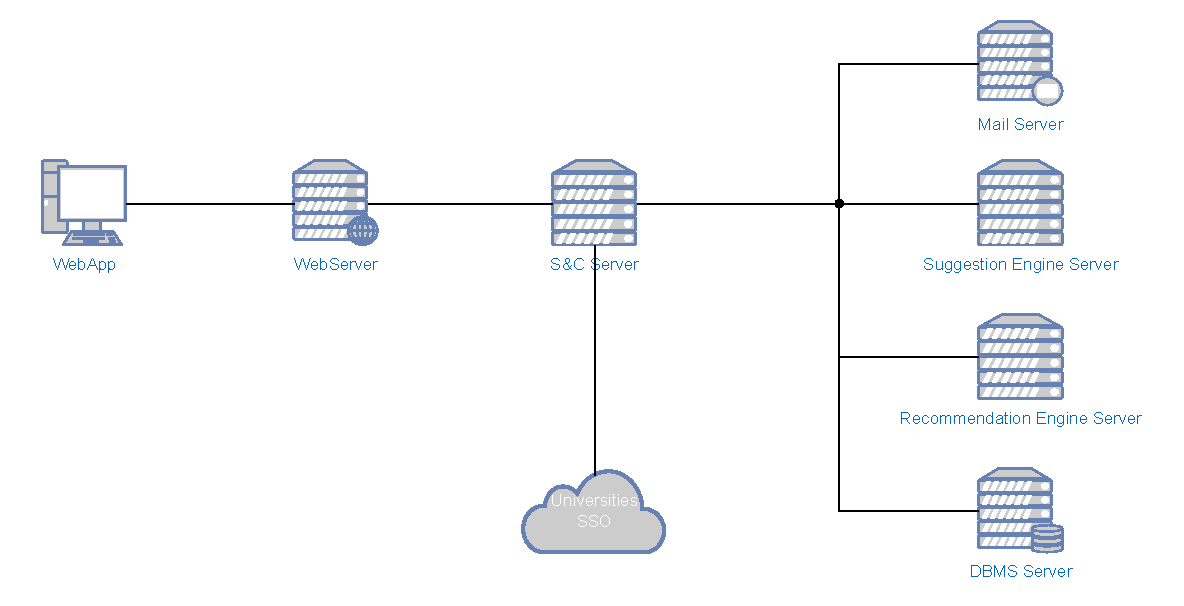
\includegraphics[width=0.85\textwidth]{Images/Overview_diagram.pdf}
      \caption{S\&C Architecture Overview}
      \label{fig:overview}
\end{figure}

\par On the client side can be seen:

\begin{itemize}
      \item \textbf{WebApp}: The web application that the user interacts with, allowing users to connect to S\&C.
            It displays the user interface and sends the user's requests to the core server.
\end{itemize}

\par On the server side, we can see:

\begin{itemize}
      \item \textbf{Web Server}: It handles communication between users and the S\&C system. It is responsible for
            serving the user interface and processing user requests by forwarding them to the S\&C Server.
            Additionally, it manages user sessions and contains the necessary configuration for student authentication
            through university Single Sign-On (SSO) services.
      \item \textbf{S\&C Server}: The main server of the S\&C system. It is the core component and is responsible
            for communication between the Web Server and the databases and the APIs/Services.
      \item \textbf{DBMS Server}: This server archives all the essential information of the system.
            It stores data related to Users, CVs, Internship Advertisements, and Complaints.
      \item \textbf{Recommendation Engine Server}: This server is responsible for generating recommended Internship
            Advertisements for students and anonymous CVs for companies.
      \item \textbf{Suggestions Engine Server}: This server is responsible for generating suggestions for improving
            students' CVs and companies' internship advertisements.
      \item \textbf{Mail Server}: This server is responsible for sending emails to users. It is used for sending
            notifications and confirmations of actions performed by users.
\end{itemize}

\section{Component View}
\label{sec:component-view}%

\subsection{High-Level Components}
\label{sub:high-level-components}%

\begin{figure}[H]
      \centering
      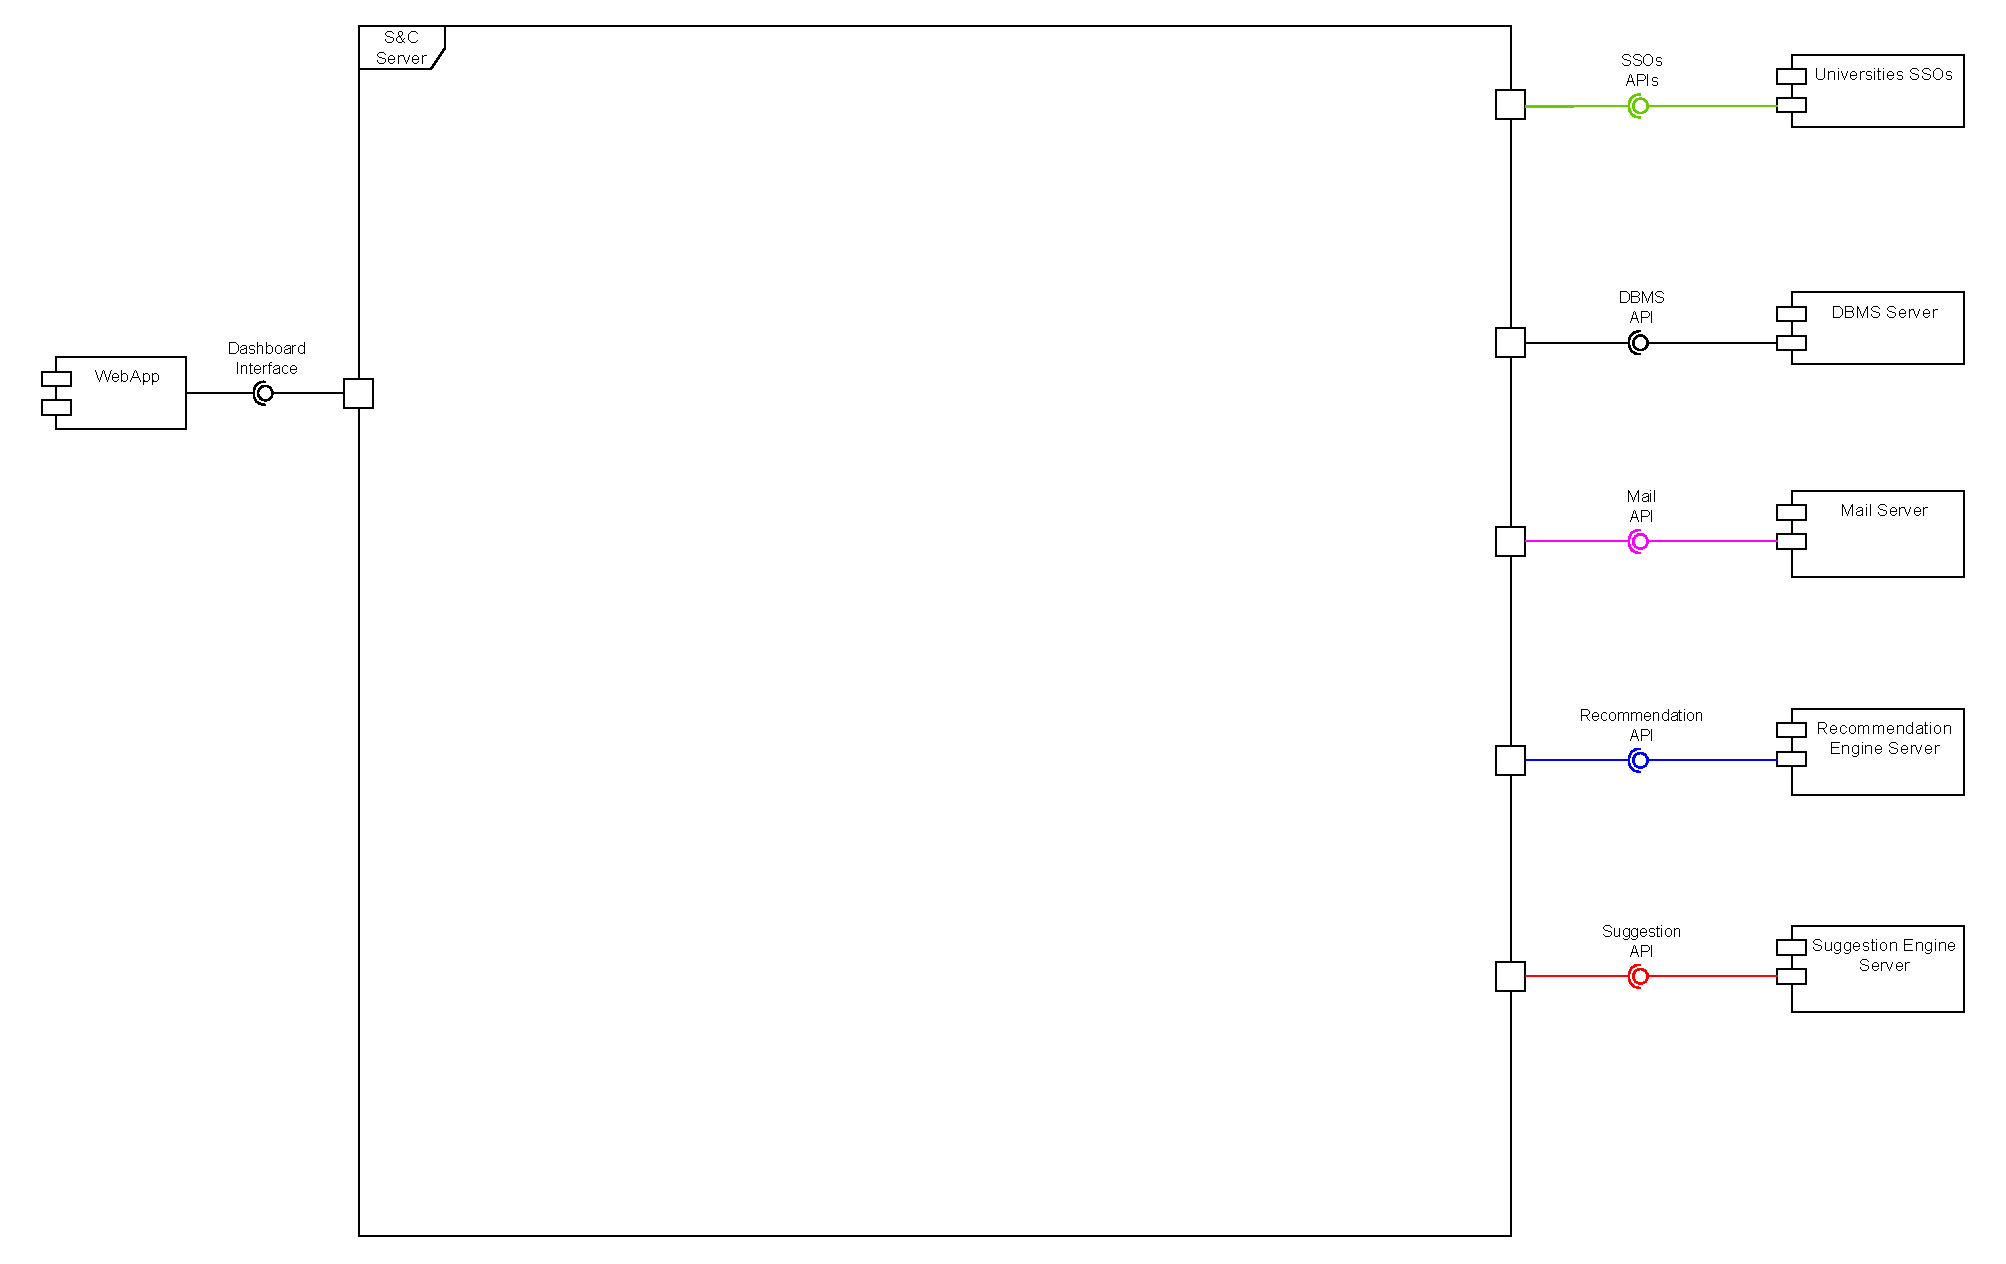
\includegraphics[width=0.85\textwidth]{Images/High_Level_Architectural_Design.pdf}
      \caption{High-Level Components}
      \label{fig:high-level-components}
\end{figure}

\par Figure \ref{fig:high-level-components} shows the high-level components of the S\&C system. The main external components are:

\begin{itemize}
      \item \textbf{WebApp}: This is the web application that the user interacts with. It allows users to communicate
            with the S\&C Server through the Dashboard Interface, which is the only means of interaction
            between the users and the system. The Dashboard Interface includes multiple functionalities,
            one of which allows the Dashboard to send notifications to users while they are using the system.
      \item \textbf{DBMS Server}: This server stores all the information of the Users, including their profile information, CVs,
            Internship Advertisements, Questionnaires, and Complaints. It is the main component of the system and is
            responsible for data management.
      \item \textbf{Mail Server}: This server is responsible for notifying users outside of the web application.
            It is used to send all types of notifications, including those confirming actions performed by a user,
            notifications of new recommendations for both students and companies, requests to fill out questionnaires,
            and notifications about the creation of new complaints, etc.
      \item \textbf{Recommendation Engine Server}: This server is responsible for generating recommended Internship Advertisements for students
            and anonymous CVs for companies. It periodically retrieves CV data and Internship Advertisement data
            to improve the program responsible for creating suggestions for each user.
      \item \textbf{Suggestions Engine Server}: This server is responsible for generating suggestions for improving students' CVs and companies' internship advertisements.
            It periodically retrieves CV data, Internship Advertisement data, and feedback answers at the end of internships
            to improve the program responsible for creating suggestions for each user.
      \item \textbf{Universities SSOs}: This external component allows students to log in to the system using their university credentials.
\end{itemize}

\subsection{Low-Level Components}
\label{sub:low-level-components}%

\begin{figure}[H]
      \centering
      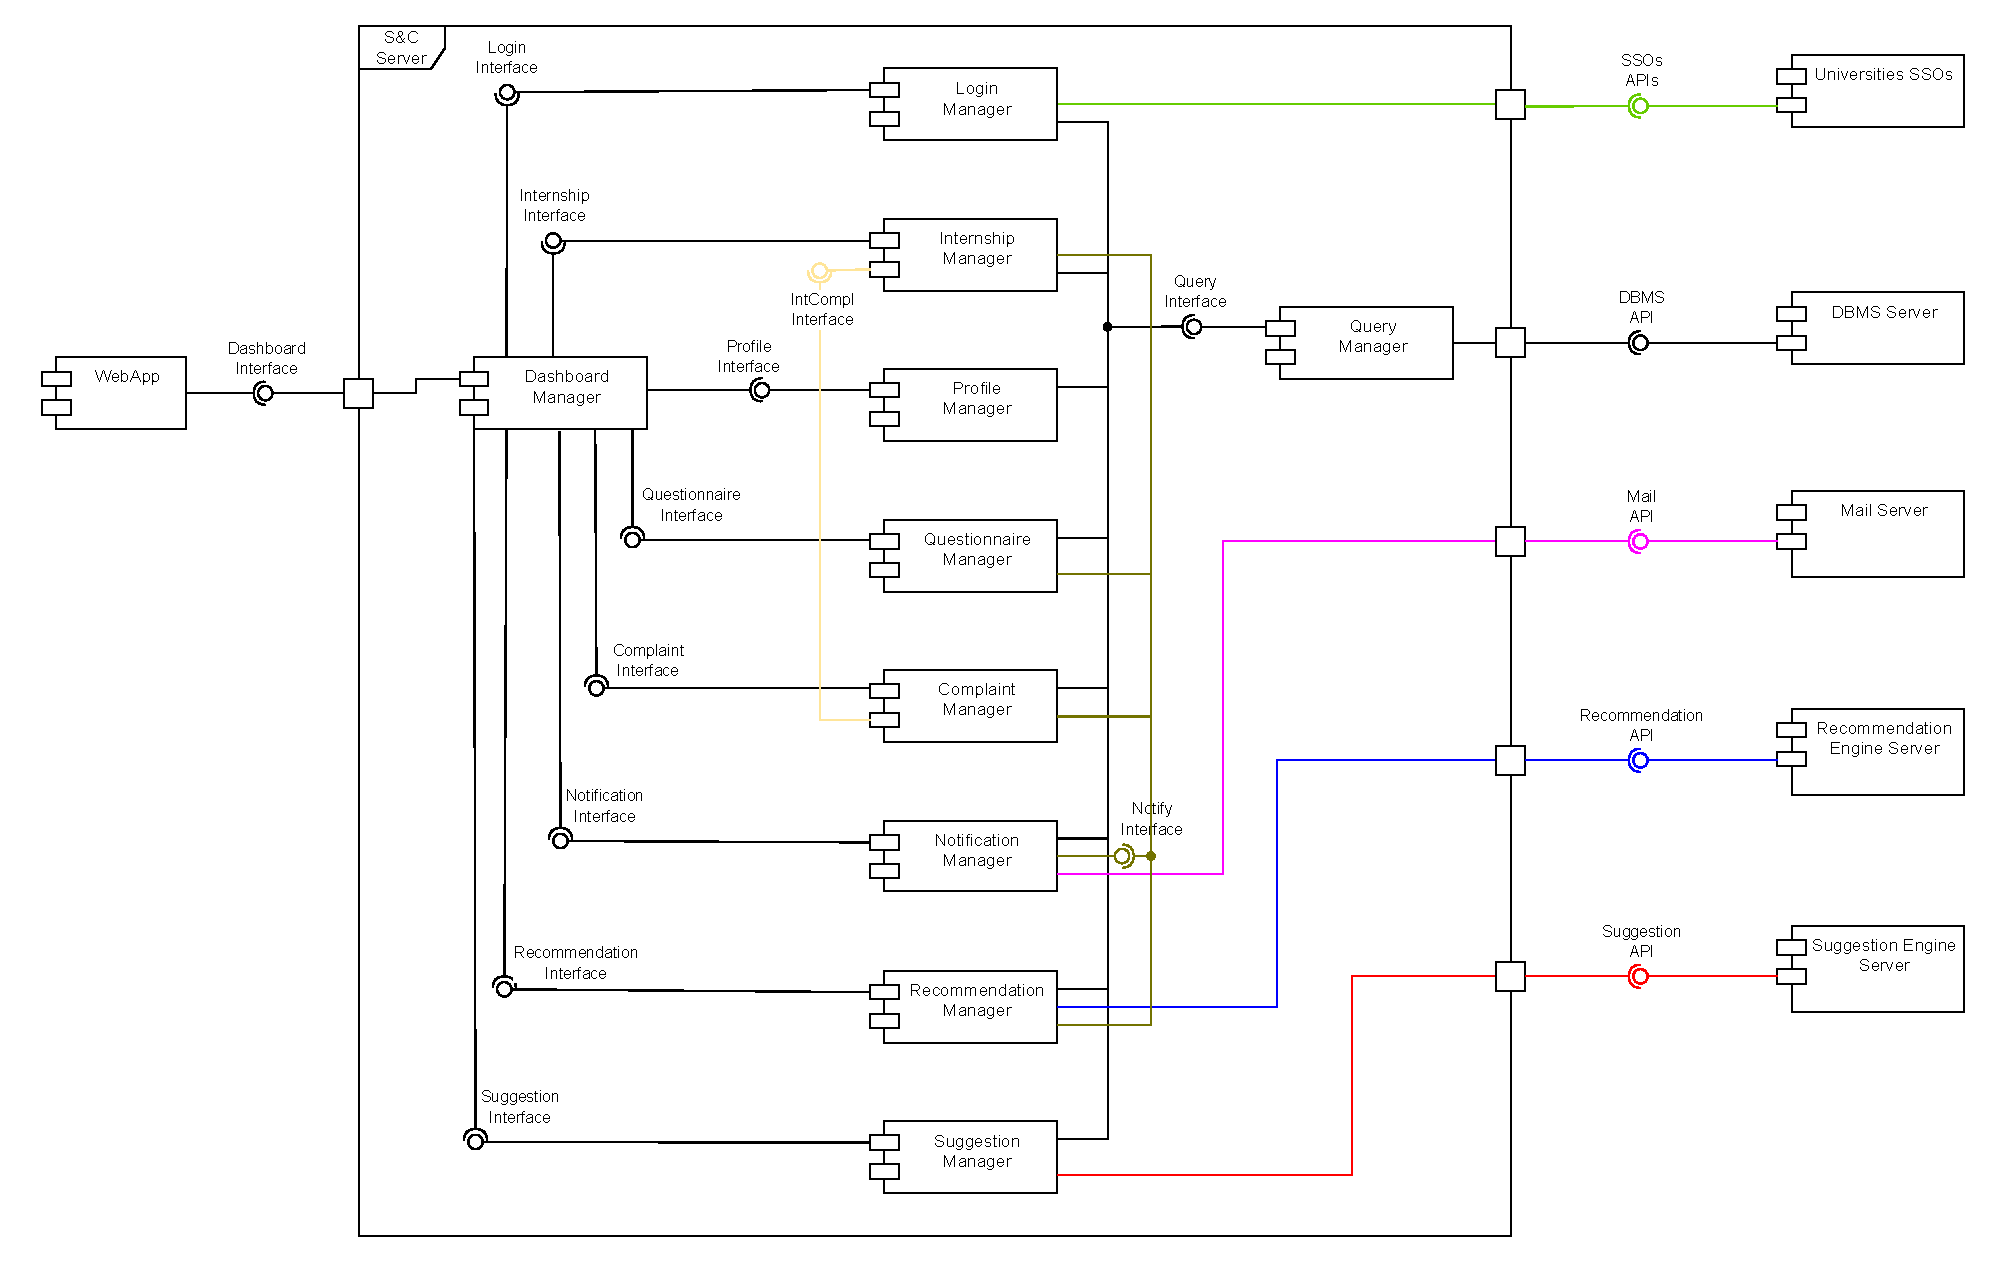
\includegraphics[width=0.85\textwidth]{Images/Low_Level_Architectural_Design.pdf}
      \caption{Low-Level Components}
      \label{fig:low-level-components}
\end{figure}

\par Figure \ref{fig:low-level-components} shows the complete architecture of the S\&C system, detailing the components inside the S\&C Server:

\begin{itemize}
      \item \textbf{Dashboard Manager}: This component is responsible for interacting with users through the dashboard interface.
            The Dashboard Manager executes user requests and interacts with the appropriate components.
      \item \textbf{Login Manager}: This component is responsible for user login. For companies it checks credentials 
      against those stored in the DBMS. For students and and universities, it interacts with the Universities SSOs,
      for the students it also handle the first access to the platform.
      \item \textbf{Internship Manager}: This component manages all stages of the Internship selection and execution process.
            It handles the creation of Internship Advertisements, the list of student applications,
            and the status of internships. It also provides an interface for the Complaint Manager to modify the status of internships.
      \item \textbf{Profile Manager}: This component manages user profiles. It allows users to modify their profile information,
            students to upload their CVs, and companies to create their profile descriptions.
      \item \textbf{Questionnaire Manager}: This component manages Questionnaires, both those created by companies for selecting students for internships
            and those created by the system for feedback at the end of internships.
      \item \textbf{Complaints Manager}: This component manages complaints. It is used to create complaints, manage them, and if necessary,
            interact with the related internship to modify its status through the interface provided by the Internship Manager.
      \item \textbf{Notification Manager}: This component manages notifications. It generates notifications to send to the
            dashboard if the user is logged in, and interacts with the Mail Server to send notifications to users outside of the web application.
      \item \textbf{Recommendation Manager}: This component interacts with the Recommendation Engine Server. It retrieves the data
            required by the recommendation engine to improve its suggestions, and retrieves the results of the recommendation engine to display to users.
      \item \textbf{Suggestions Manager}: This component interacts with the Suggestions Engine Server. It retrieves the data
            required by the suggestion engine to improve its suggestions, and retrieves the results of the suggestion engine to display to users.
      \item \textbf{Query Manager}: This component executes queries and converts the data returned by the DBMS into the necessary objects for other components.
\end{itemize}

\subsubsection{Login Manager}
\label{subsub:login-manager}%

\begin{figure}[H]
      \centering
      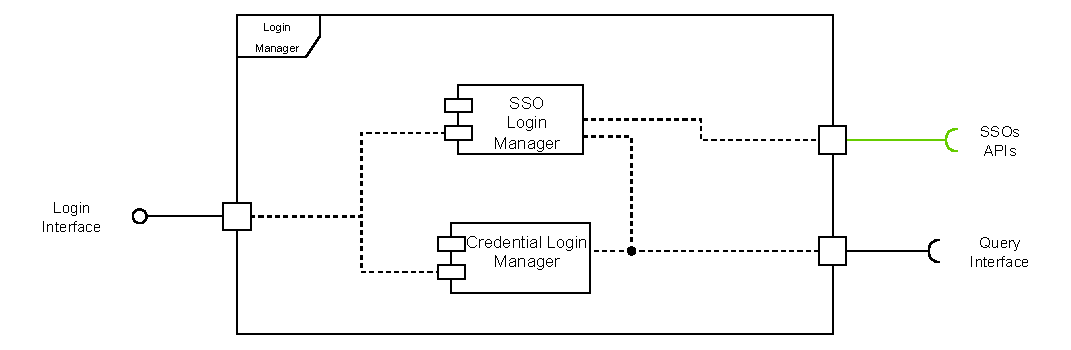
\includegraphics[width=0.85\textwidth]{Images/Login_Architecture.pdf}
      \caption{Login Manager}
      \label{login-manager-arch}
\end{figure}

\par The Login Manager is composed of other two sub-components:
\begin{itemize}
      \item \textbf{SSO Login Manager}: This component is responsible for interacting with the Universities SSOs to authenticate 
      the students and the authorized staff with the SSOs. It also manages the registration of new students. 
      It creates a new student profile if the student is not already registered in the DBMS.
      \item \textbf{Credential Login Manager}: This component is responsible for authenticating the company with the credentials
      stored in the DBMS. 
\end{itemize}

\subsubsection{Internship Manager}
\label{subsub:internship-manager}%

\begin{figure}[H]
      \centering
      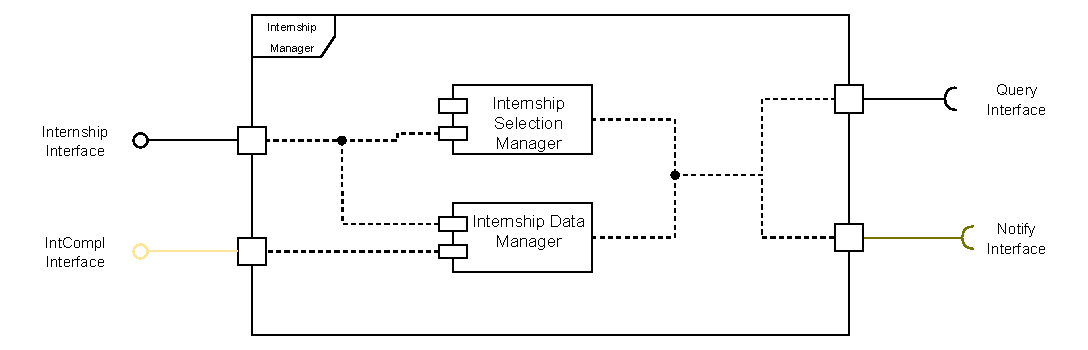
\includegraphics[width=0.85\textwidth]{Images/Internship_Architecture.pdf}
      \caption{Internship Manager}
      \label{internship-manager-arch}
\end{figure}

\par The Internship Manager is composed of other two sub-components:
\begin{itemize}
      \item \textbf{Internship Selection Manager}: This component is responsible all the stages of the internship selection process.
            It handles the creation of internship advertisements, the list of student applications.
      \item \textbf{Internship Data Manager}: This component is responsible for managing the status of internships,
            who's the responsible for the internship, the descriptions of it, the requirements and the duration.
            It also provides an interface for the Complaint Manager to modify the status of internships.
\end{itemize}

\subsubsection{Profile Manager}
\label{subsub:profile-manager}%

\begin{figure}[H]
      \centering
      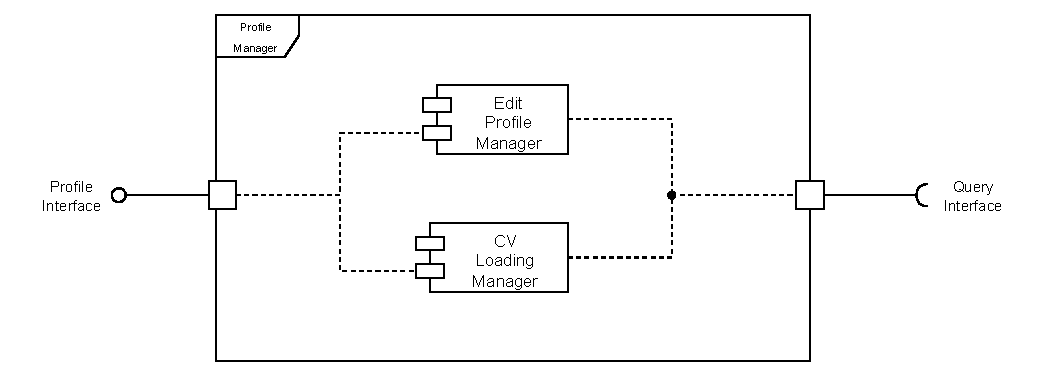
\includegraphics[width=0.85\textwidth]{Images/Profile_Architecture.pdf}
      \caption{Profile Manager}
      \label{profile-manager-arch}
\end{figure}

\par The Profile Manager is composed of other two sub-components:
\begin{itemize}
      \item \textbf{Profile Manager}: This component is responsible for the modification of the user's profile information.
            For the companies it allows to create their profile description that will be shown to students.
      \item \textbf{CV Manager}: This component is responsible for the management of the student's CVs and uploading them.
\end{itemize}

\subsubsection{Questionnaire Manager}
\label{subsub:questionnaire-manager}%

\begin{figure}[H]
      \centering
      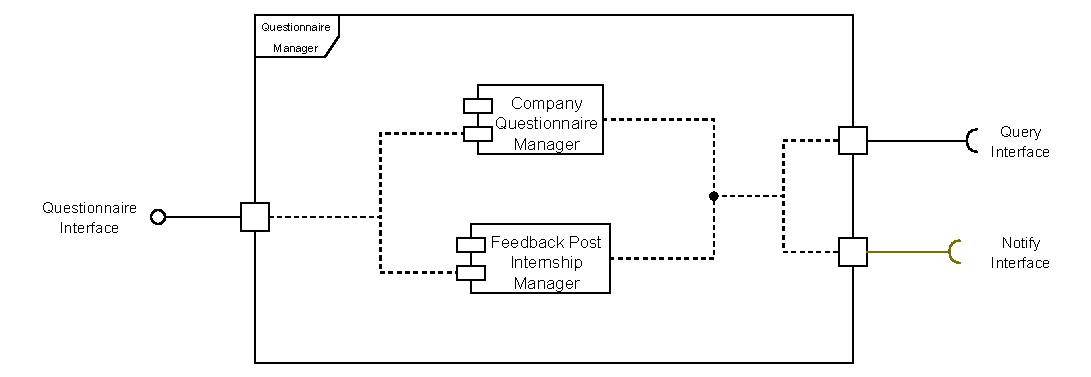
\includegraphics[width=0.85\textwidth]{Images/Questionnaire_Architecture.pdf}
      \caption{Questionnaire Manager}
      \label{questionnaire-manager-arch}
\end{figure}

\par The Questionnaire Manager is composed of other two sub-components:
\begin{itemize}
      \item \textbf{Company Questionnaire Manager}: This component is responsible for managing the questionnaires created by companies.
            It allows companies to create, modify and delete questionnaires to select students for internships.
            It allows companies to see the answers to the questionnaires.
      \item \textbf{Feedback Questionnaire Manager}: This component is responsible for managing the feedback questionnaires created by the system.
            It allows the system to create questionnaires for feedback at the end of internships.
\end{itemize}

\section{Deployment View}
\label{sec:deployment-view}%

\begin{figure}[H]
      \centering
      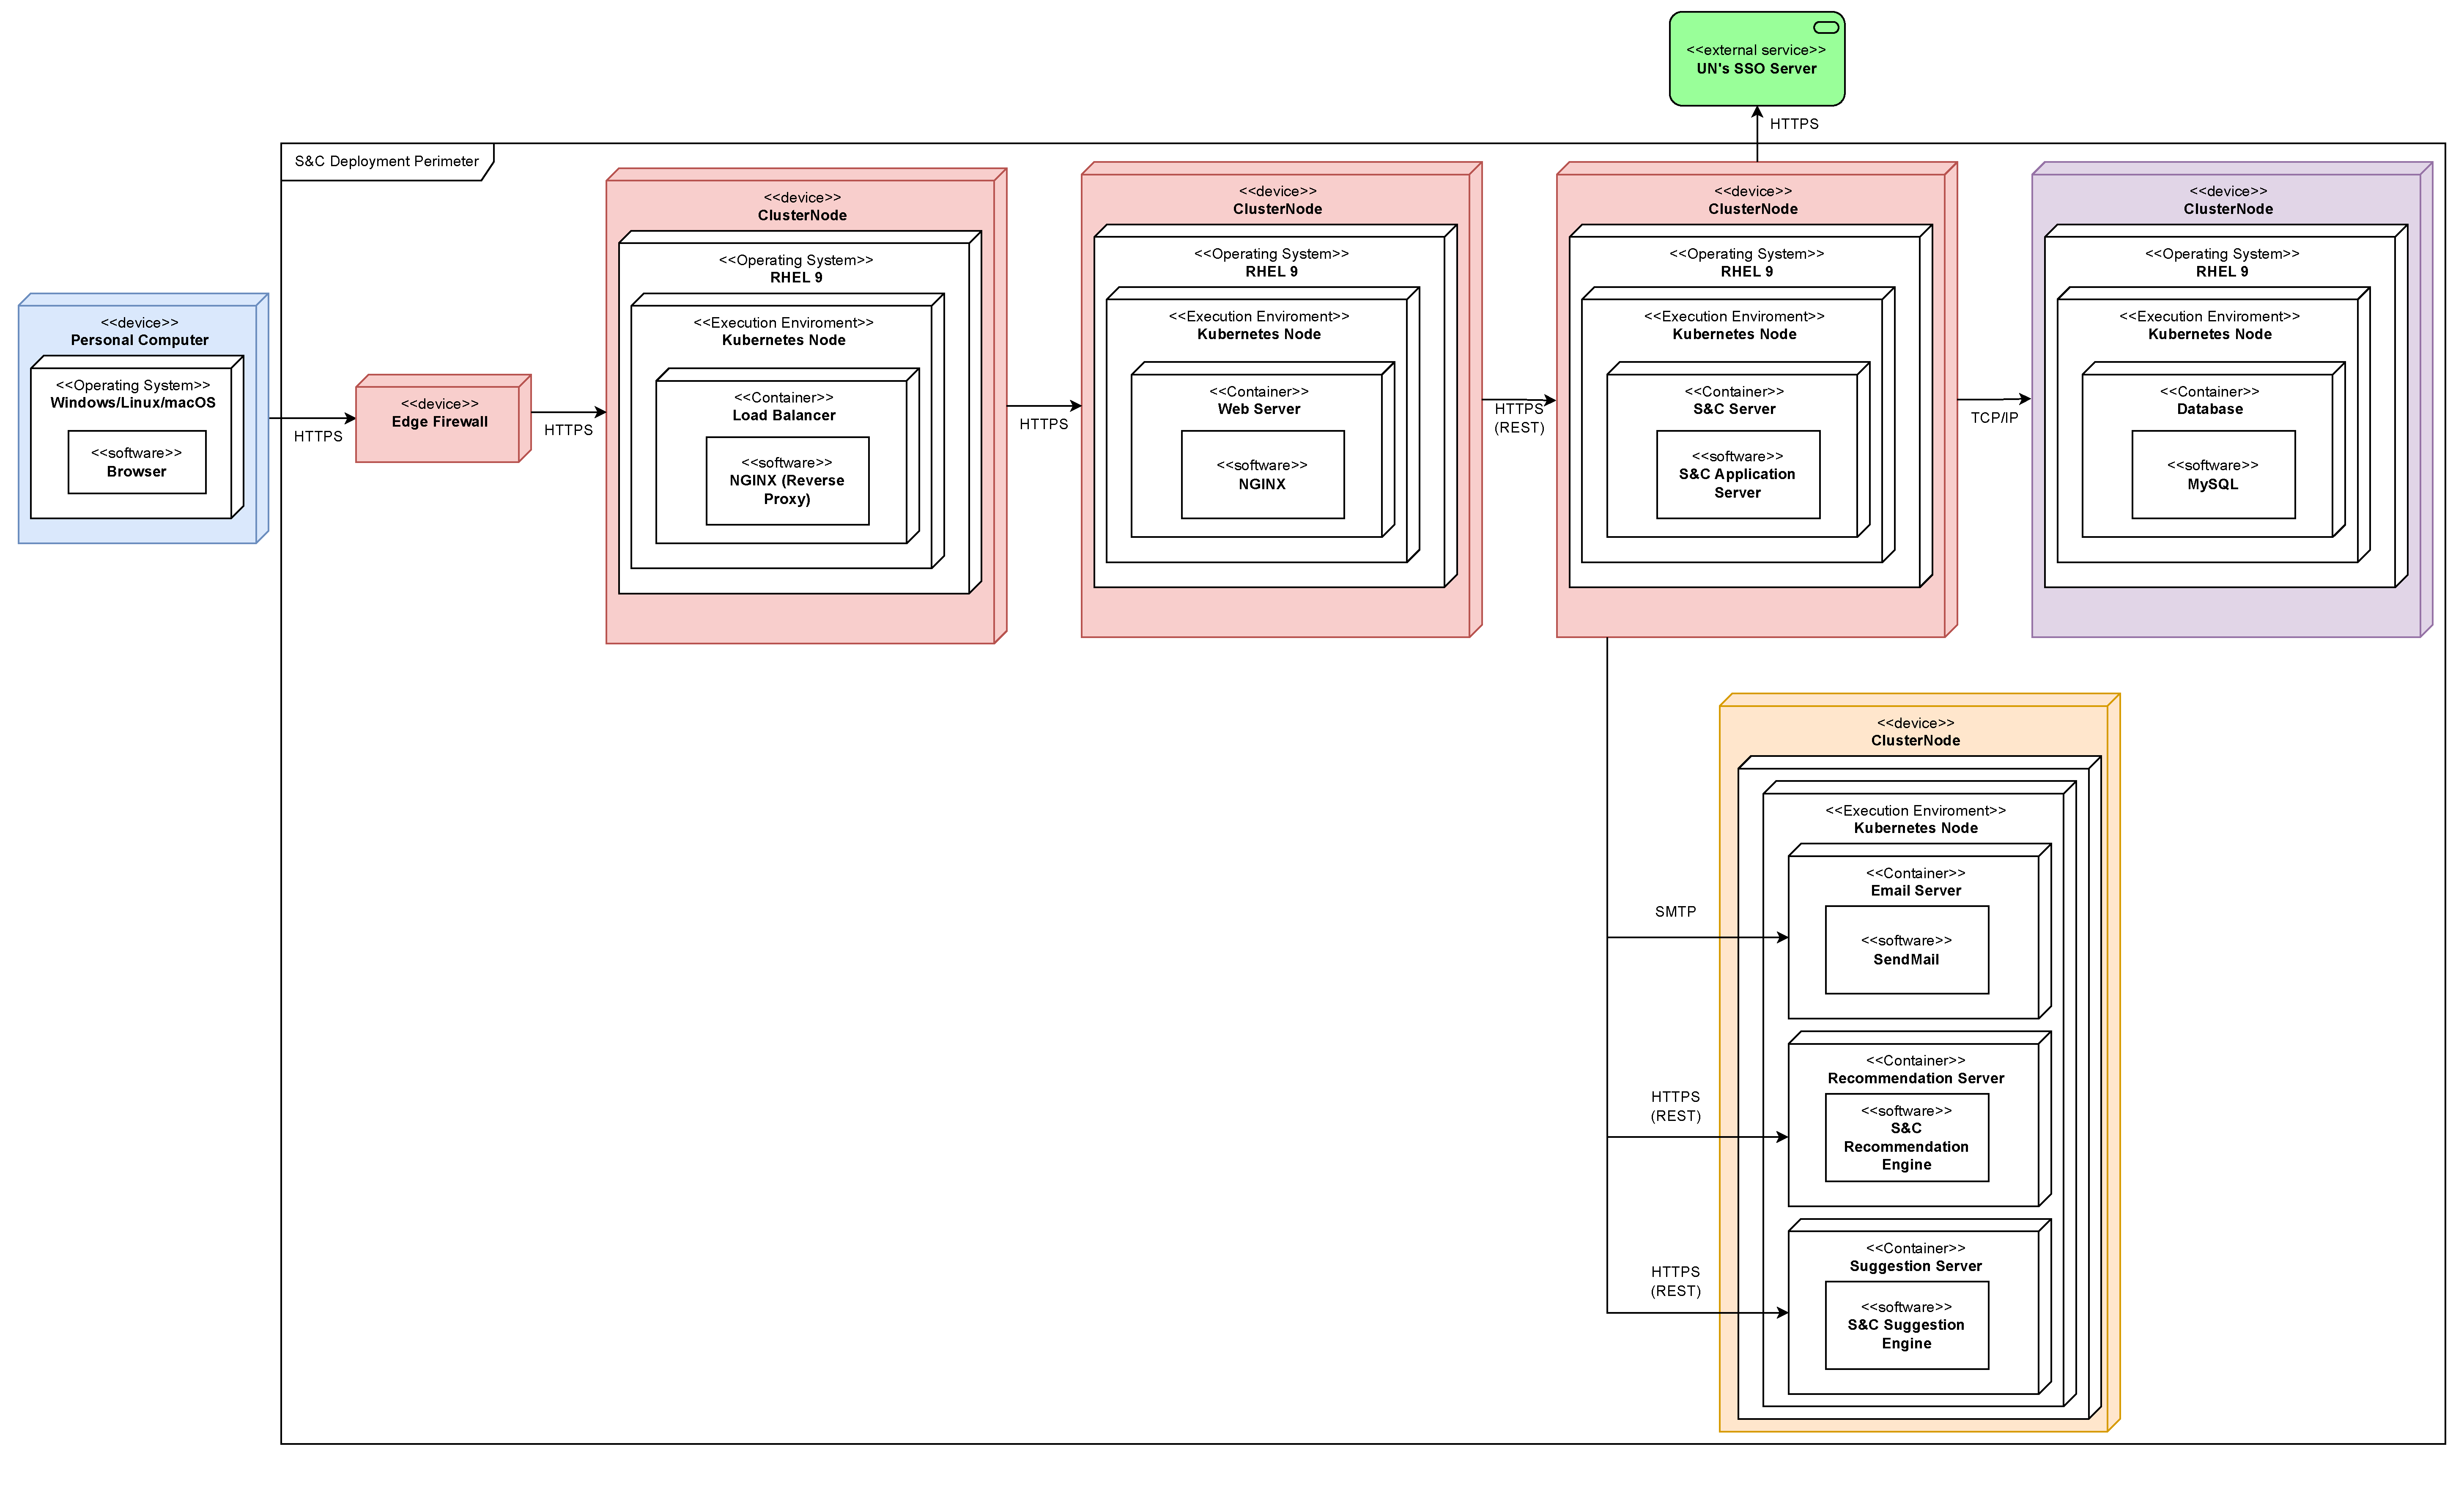
\includegraphics[width=0.85\textwidth]{Images/Deployment_Diagram.pdf}
      \caption{Deployment Diagram}
      \label{fig:deployment-diagram}
\end{figure}

\par The figure shows the deployment diagram of the S\&C infrastructure. Running on the cluster are all the components
previously described in \ref{sec:overview} each one encapsulated in independent containers.

\par Notable additions are the Load Balancer and a Firewall. The Load Balancer is responsible for distributing the
incoming traffic across the various Web Servers. The Firewall is responsible for filtering the incoming traffic and
protecting the system from malicious attacks.

\par It must be noted that all the various services are running in containers on generic x86 hardware.
The configuration shown is just an example and can be easily scaled: in a testing environment, all the services can run
on the same machine, while in a production environment, the services can be distributed across $n$ machines to improve
performance and reliability. In production, enough replicas of each service should be running to ensure high
availability.

\par The system can be easily be implemented in bare-metal hardware or in a cloud environment of choice (e.g. AWS, Azure,
Google Cloud, etc.). Multi-cloud deployment is also possible: no components are tied to a specific cloud provider or
running specific hardware. Even the firewall(s) can be virtualized if needed.

\par The rationale behind the division of the system into the various components and the chosen communication
protocols will be discussed in \ref{sec:selected-architectural-styles-patterns}. Other minor design decisions will be
explained in \ref{sec:other-design-decisions}.

\section{Runtime View}
\label{sec:runtime-view}%

\subsection{Student and Universities Staff Login}
\label{sub:student-and-universities-staff-login}%

\begin{figure}[H]
      \centering
      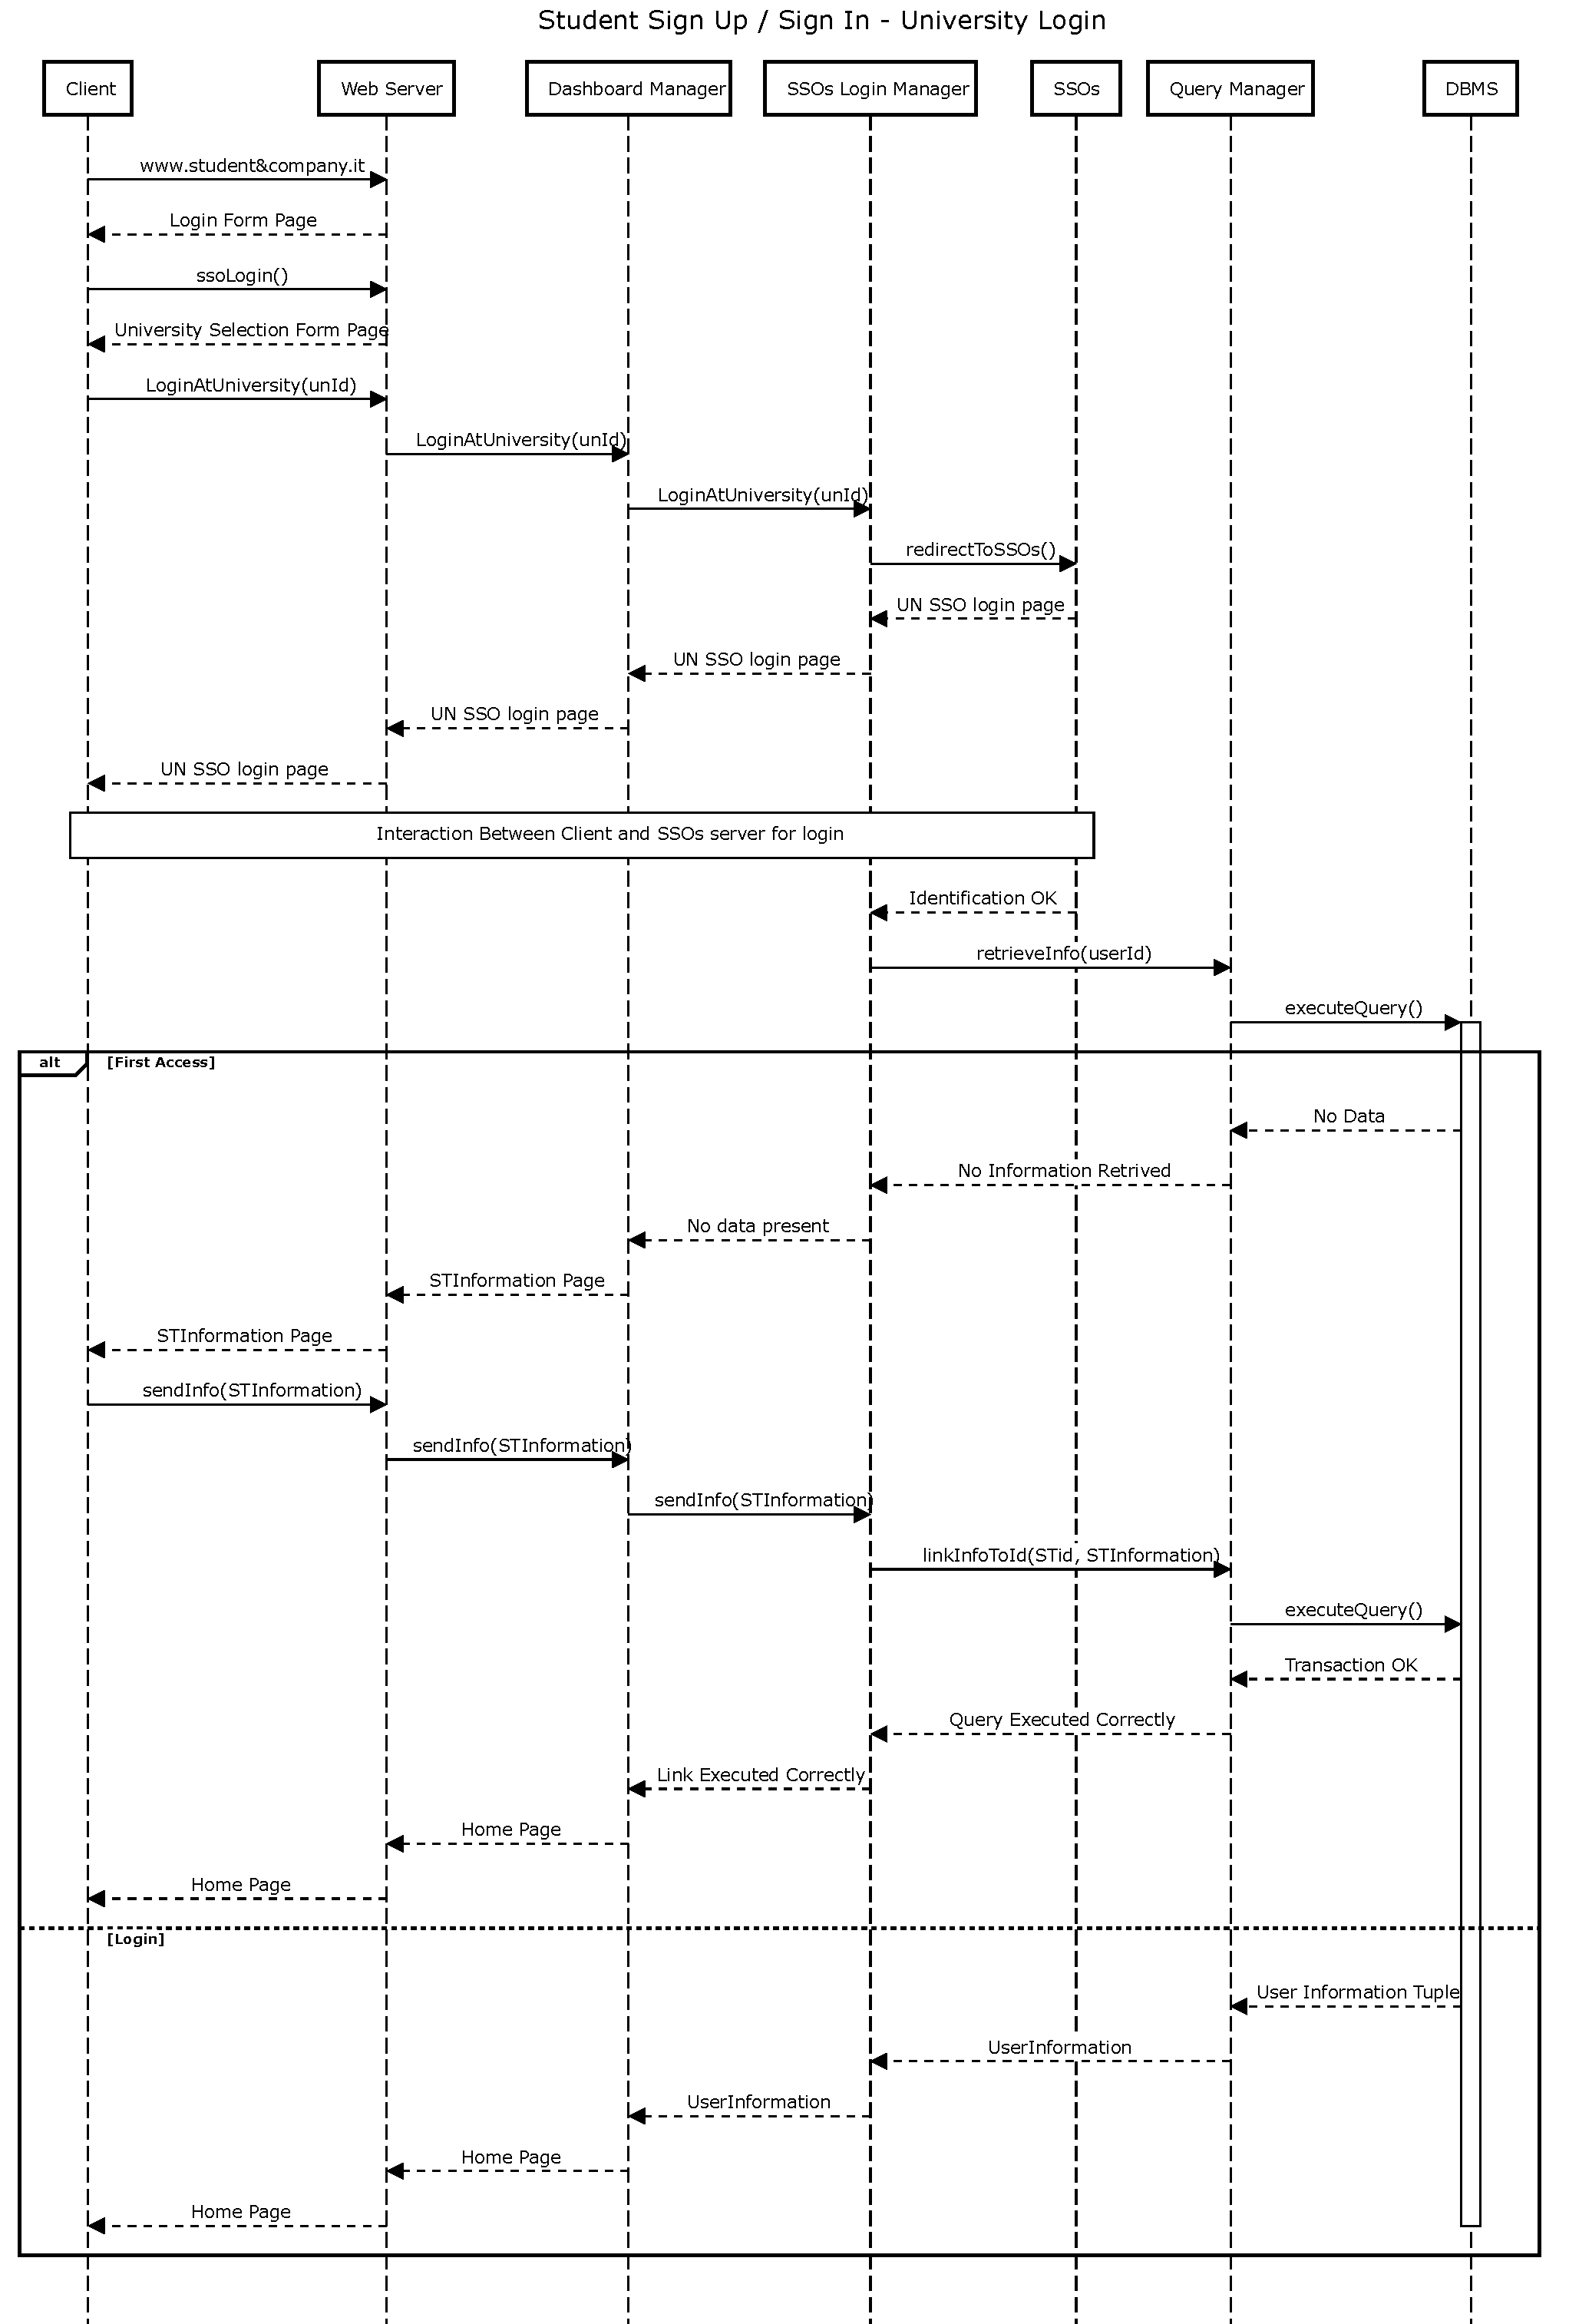
\includegraphics[width=0.85\textwidth]{Images/RV_01a.pdf}
      \caption{Runtime View - Student and Universities Staff Login}
      \label{fig:rv-student-login}
\end{figure}

\par This sequence diagram represents the ST login and first access process. The ST searches into the browser for the
S\&C web application and gets the login page. After clicking on the "Login with SSO" button the ST is redirected to
a page require the selection of the university of the ST between the available ones. After the selection, the ST is redirected
to the university's SSO page where the ST inserts the credentials. The SSO validates the credentials and sends back a
token to the S\&C server. The S\&C server validates the token and check if the ST is already registered in the system searching
for it in the DBMS. If the ST is not registered, the S\&C server creates a new ST profile and redirects the ST to the
profile page to complete the registration. If the ST is already registered, the S\&C server redirects the ST to the
dashboard page.
This process is the same for the UN staff but there is no registration process because the UN staff is registered by the S\&C staff.

\subsection{Company Login}
\label{sub:company-login}%

\begin{figure}[H]
      \centering
      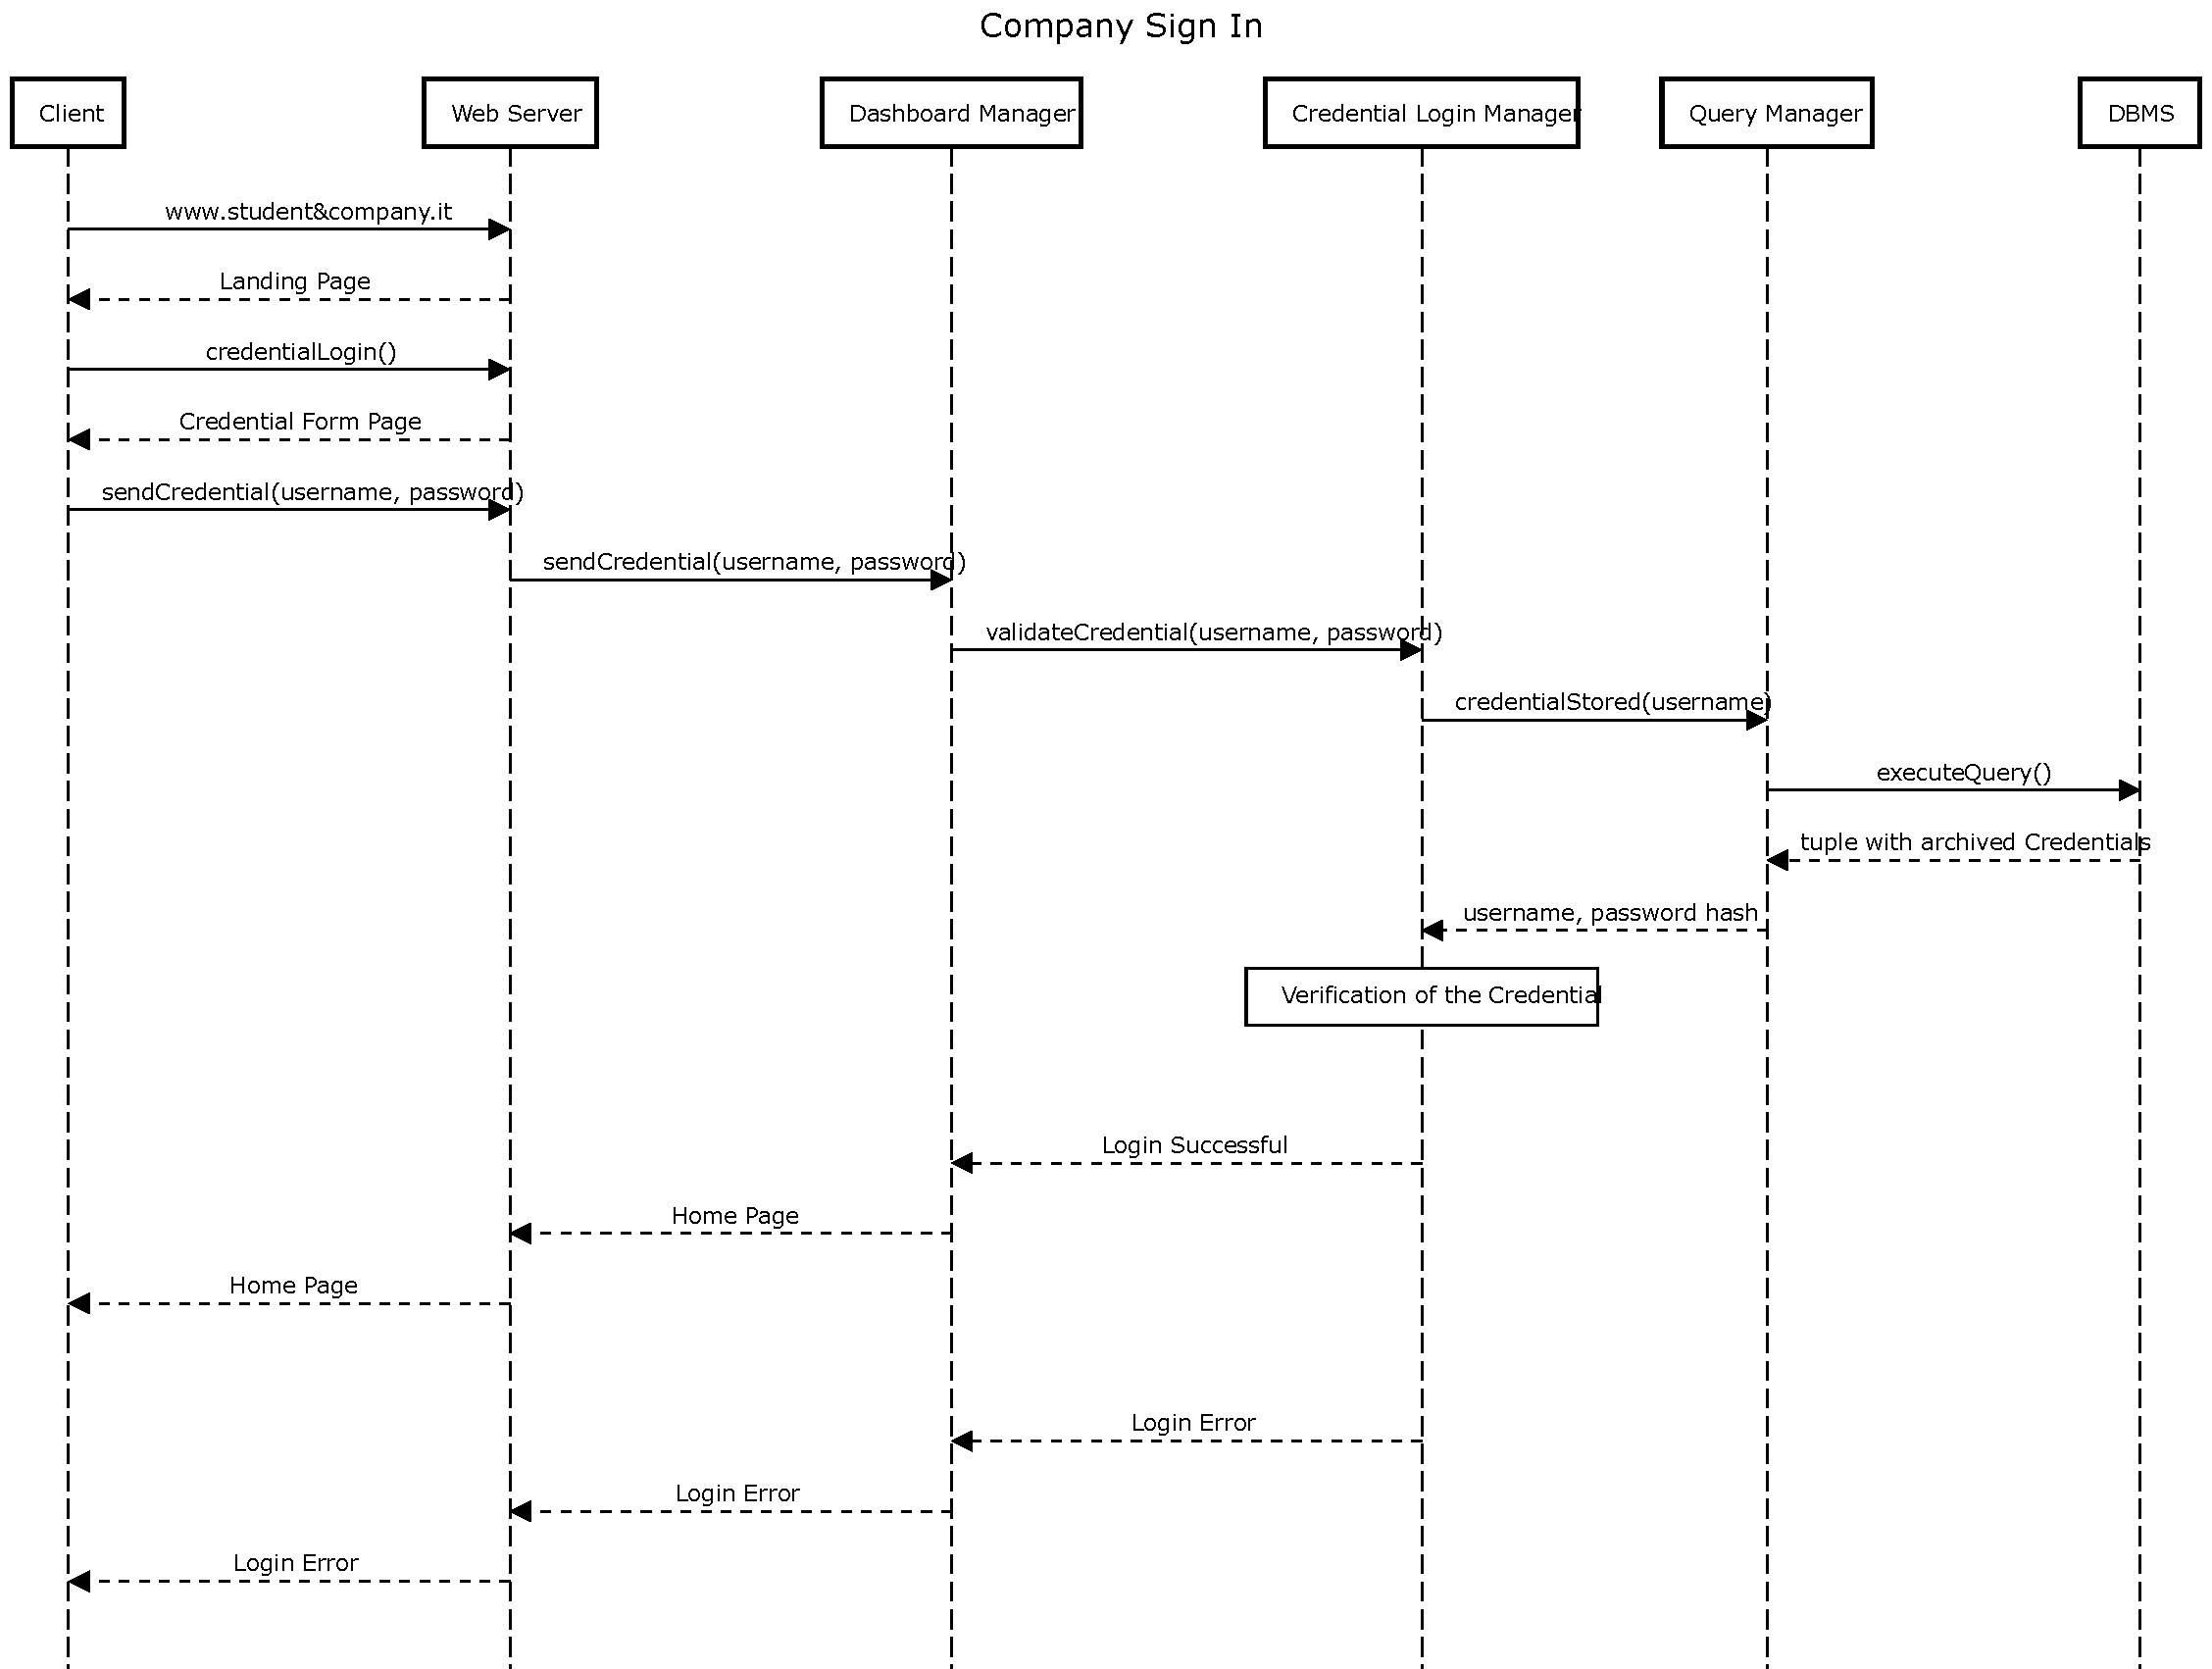
\includegraphics[width=0.85\textwidth]{Images/RV_01b.pdf}
      \caption{Runtime View - Company Login}
      \label{fig:rv-company-login}
\end{figure}

\par This sequence diagram represents the CO login process. Here is not shown the registration process because it was done
in a previous instance between the CO and the S\&C staff by email. The CO searches into the browser for the S\&C 
web application and gets the login page. After clicking on the "Login with Company credentials" button the CO 
inserts the credentials and clicks on the "Login" button. The S\&C server validates the credentials and if the credentials
are correct the CO is redirected to the dashboard page otherwise an error message is shown.

\subsection{Student Loads CV}
\label{sub:student-loads-cv}%

\begin{figure}[H]
      \centering
      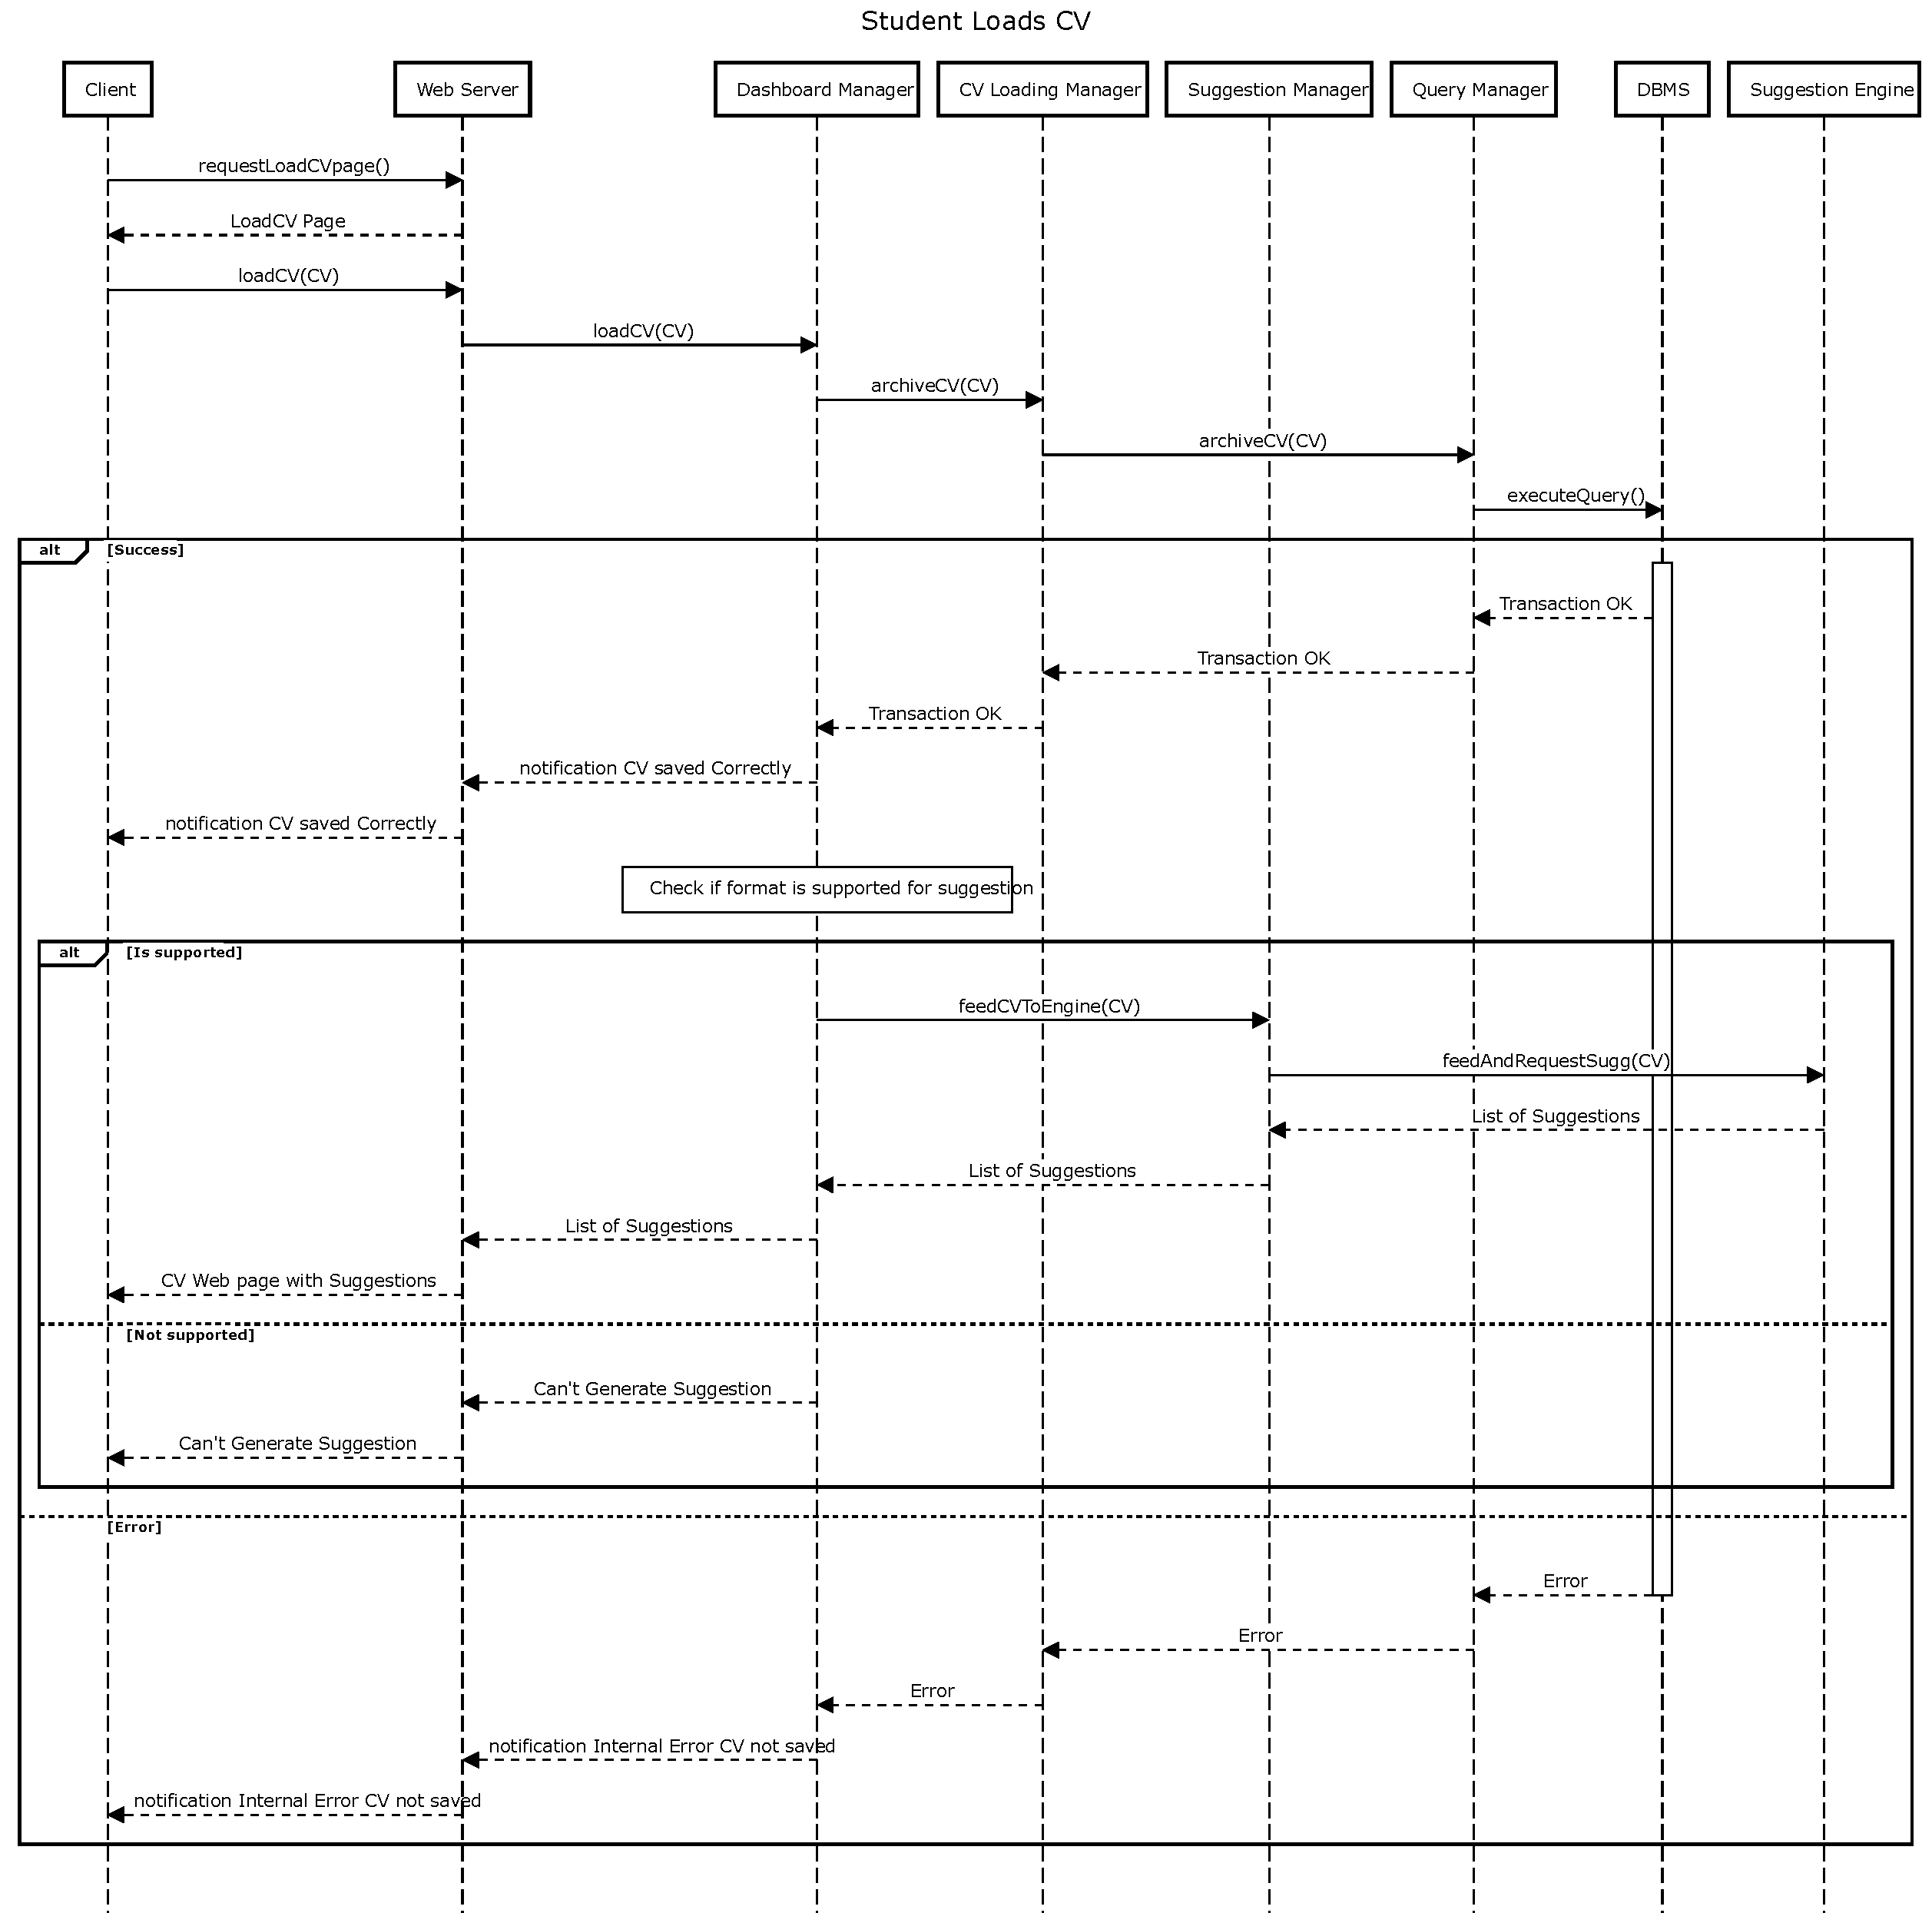
\includegraphics[width=0.85\textwidth]{Images/RV_02.pdf}
      \caption{Runtime View - Student Loads CV}
      \label{fig:rv-student-loads-cv}
\end{figure}

\par This sequence diagram represents the ST CV upload process. The ST clicks on the "Upload CV" button in his profile
management page. The S\&C server sends back the CV upload page. The ST selects the CV file and clicks on the "Upload" button.
The S\&C server validates the file and saves it in the DBMS and notifies the ST that the CV has been uploaded successfully
otherwise an error message is shown. If the CV is uploaded successfully the S\&C server checks if the CV is one of the
standard formats supported by the Suggestion Engine, if it's not then a notification is sent that the CV is not supported and
so the ST can't receive suggestions, instead if the CV is supported it's sent to the Suggestion Engine to be analyzed and
suggestions are sent back to the ST.

\subsection{Student browser and search for internships}
\label{sub:student-browser-and-search-for-internships}%

\begin{figure}[H]
      \centering
      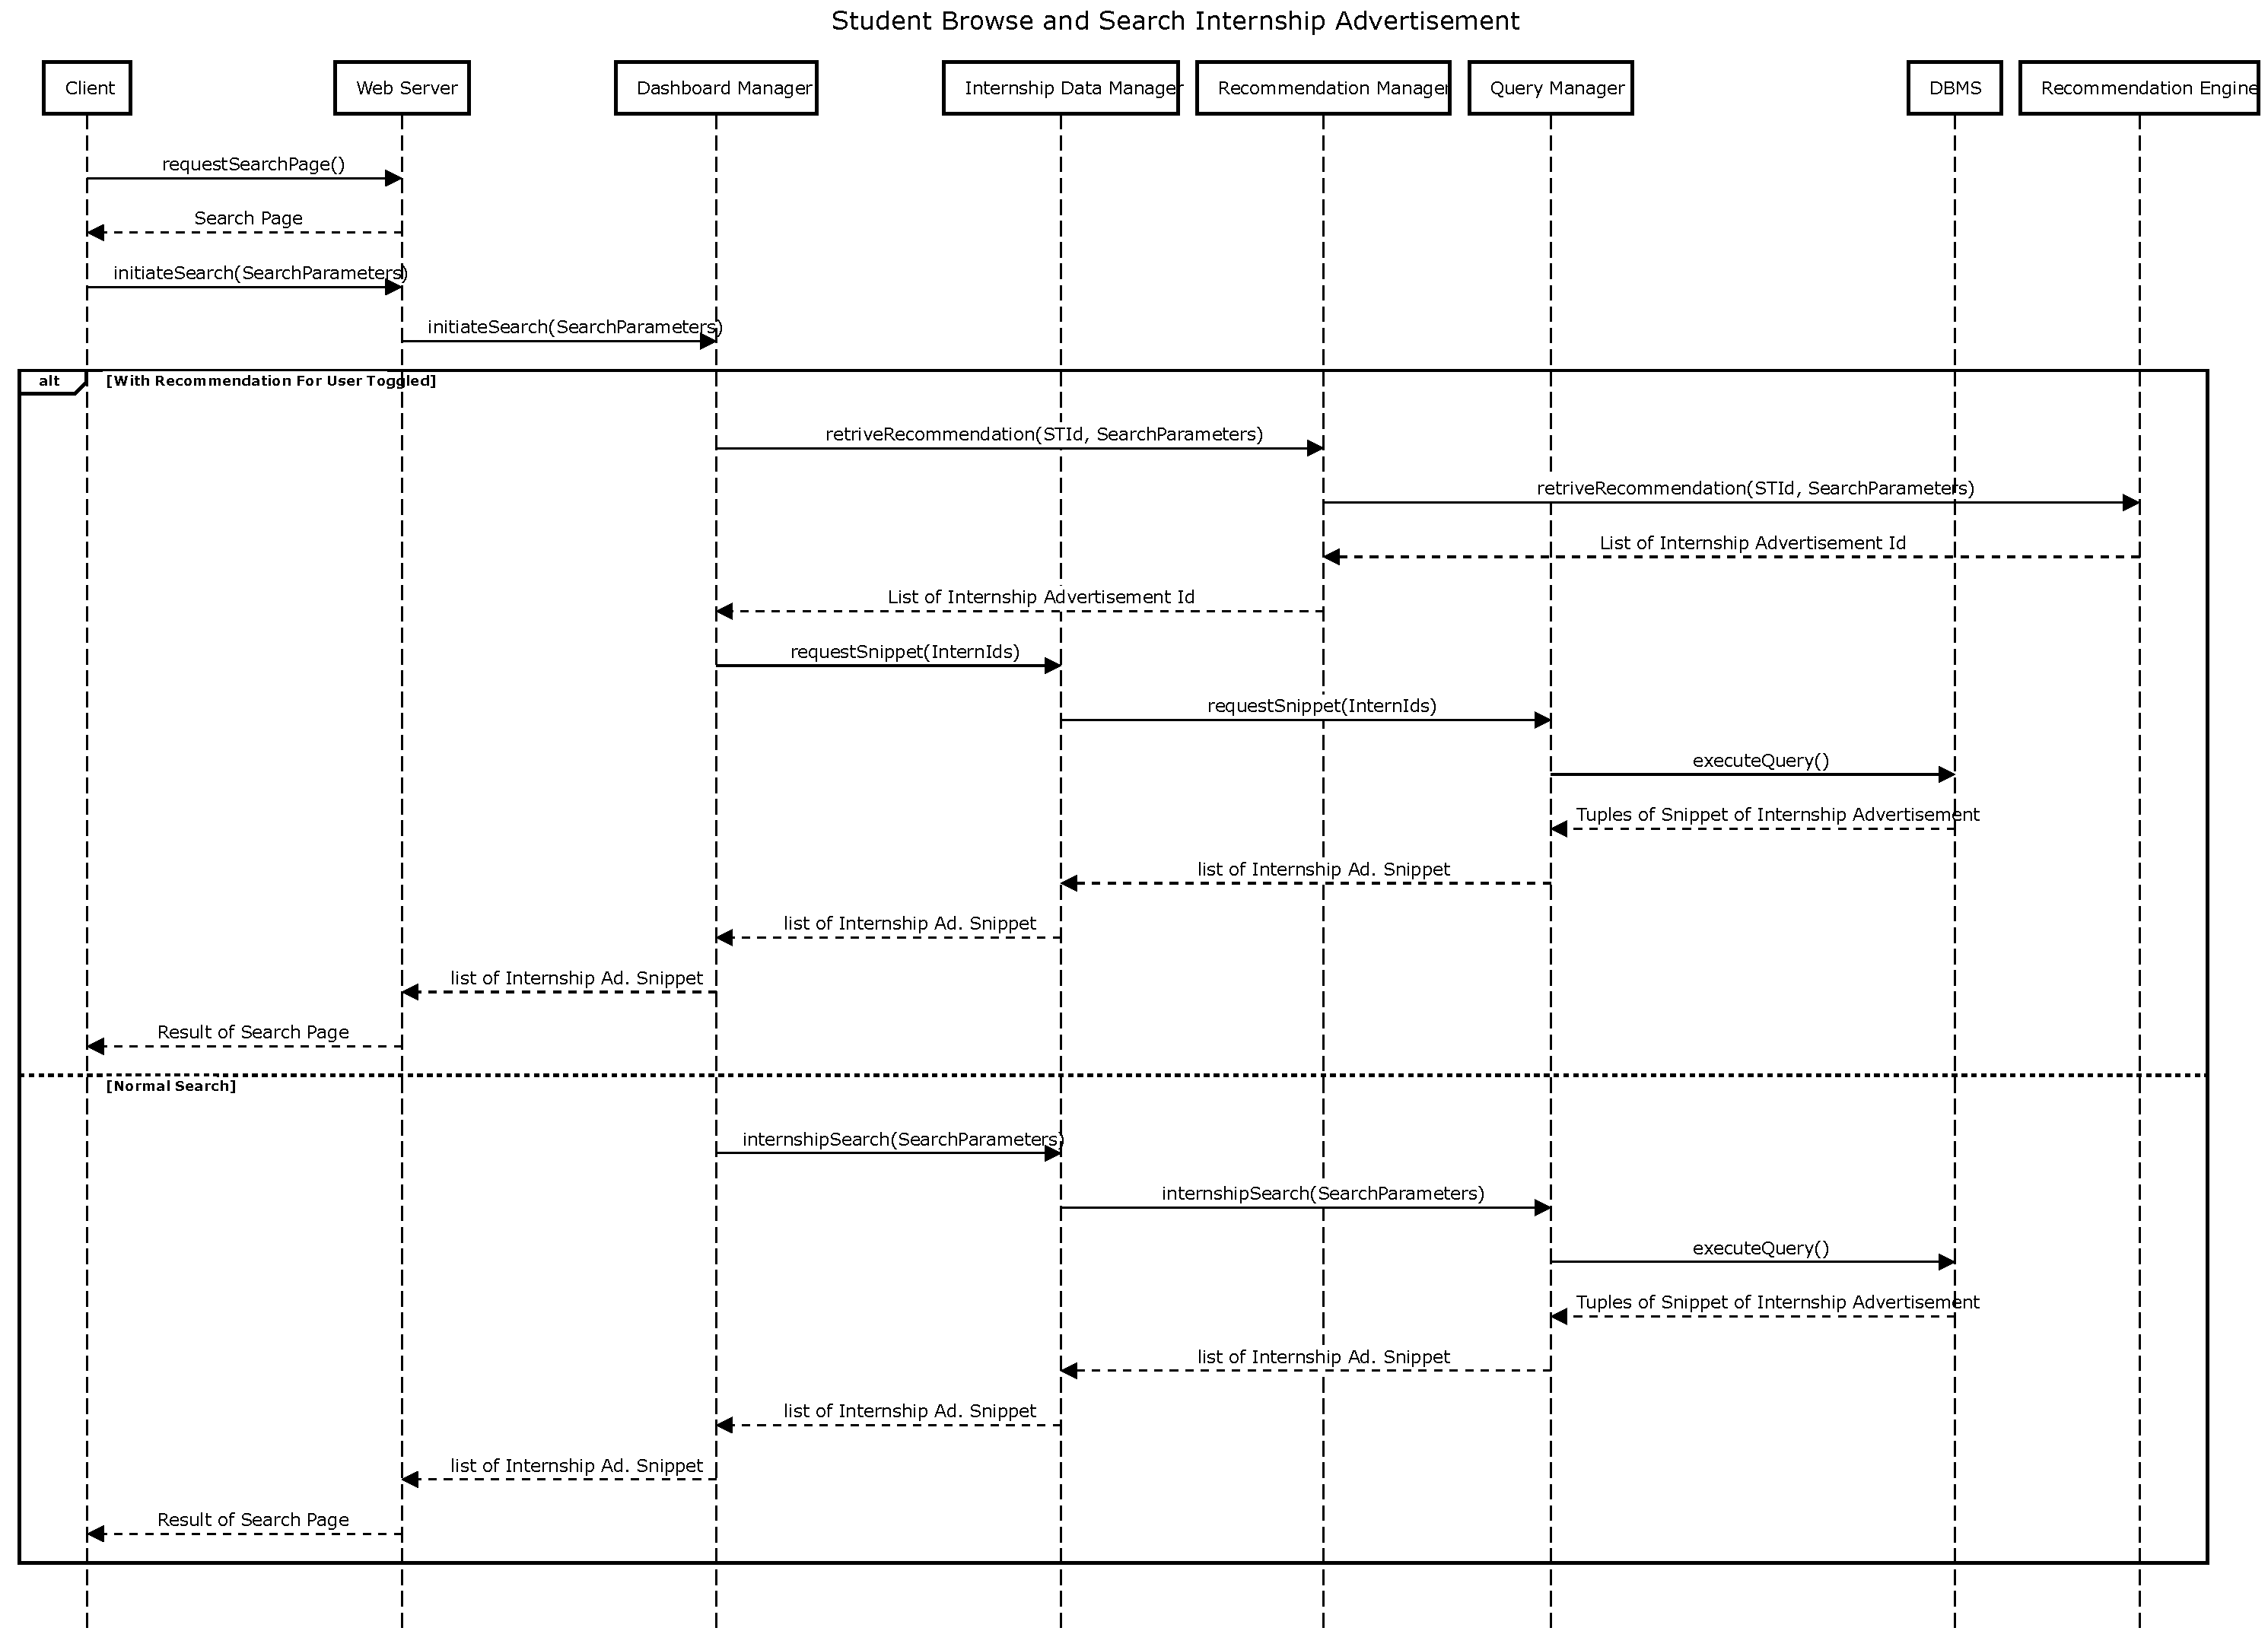
\includegraphics[width=0.85\textwidth]{Images/RV_03.pdf}
      \caption{Runtime View - Student browser and search for internships}
      \label{fig:rv-student-browser-and-search-for-internships}
\end{figure}

\par This sequence diagram represents the ST search for internships process. ST clicks on the "Search" button in the dashboard
page. The S\&C server sends back the search page. The ST selects the filters and clicks on the "Search" button. The S\&C server
through the Internship Manager retrieves the internships that match the filters and sends them back to the ST. The ST can
request the internship that the Recommendation Engine suggests to him by clicking on the "recommended for you" filter in the
filter selection. The S\&C server retrieve the recommended internships from the Recommendation Engine and sends them back to the ST.

\subsection{Student compiles Company Questionnaire}

\begin{figure}[H]
      \centering
      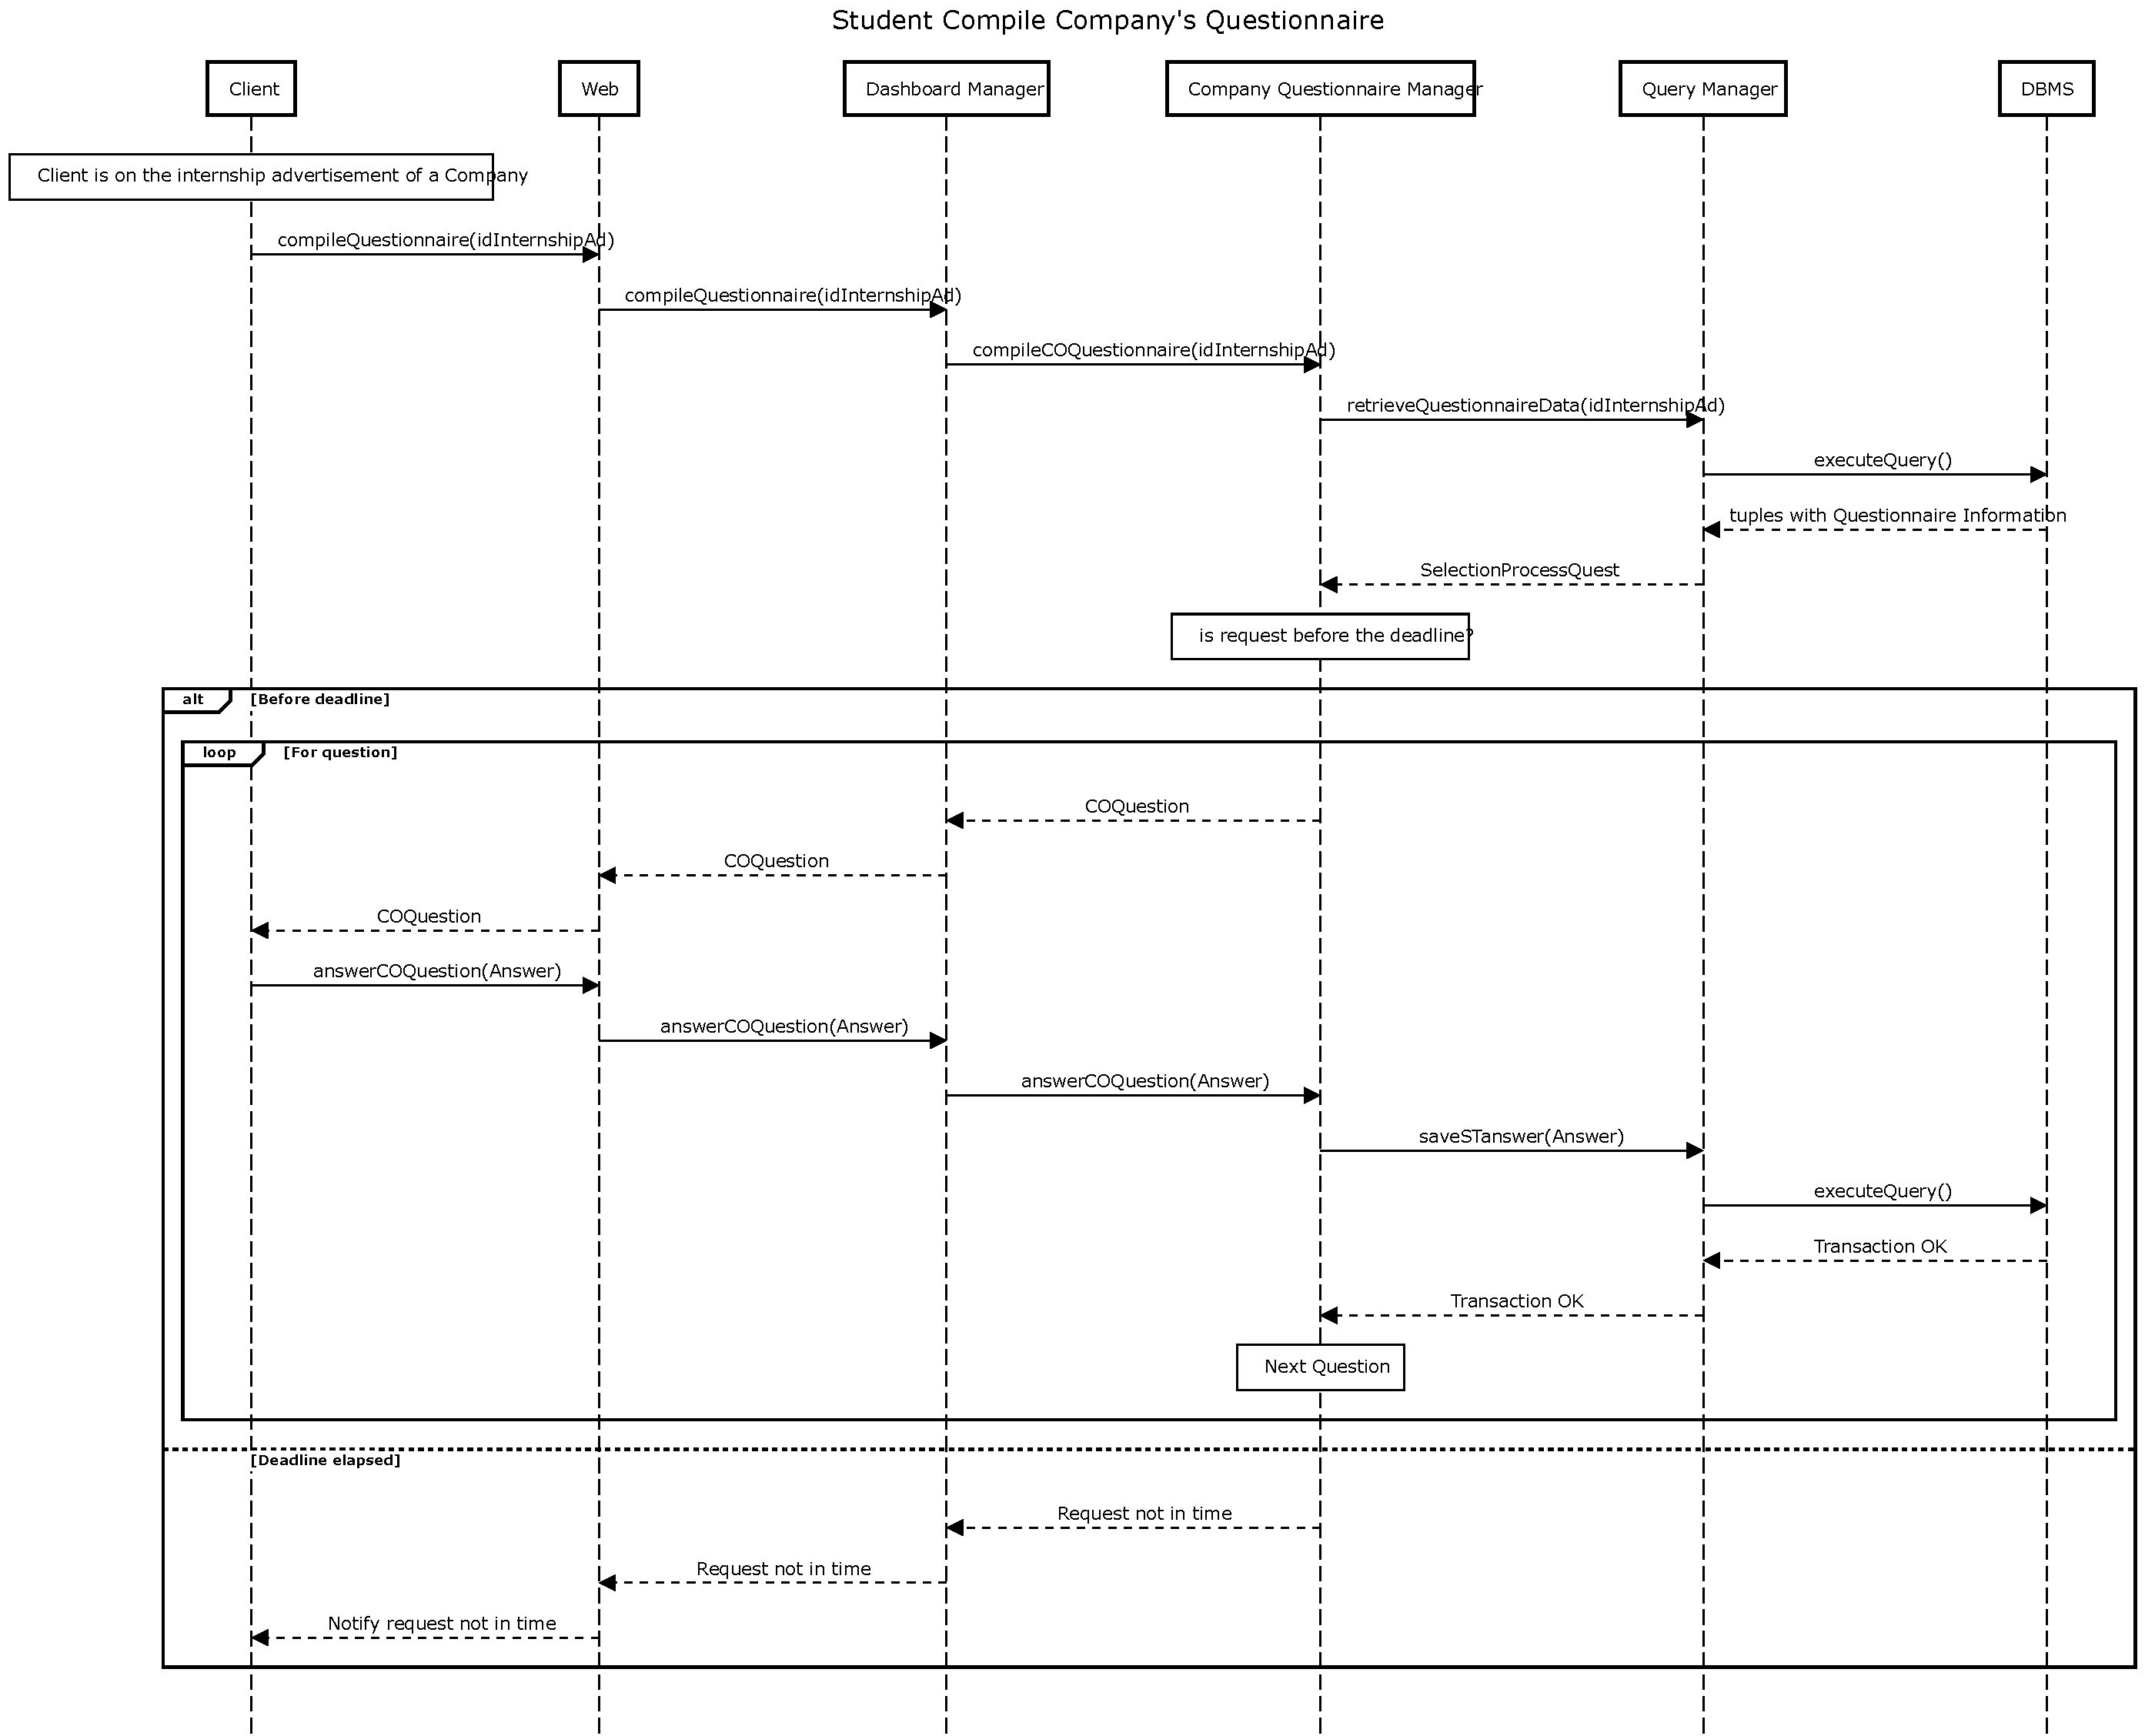
\includegraphics[width=0.85\textwidth]{Images/RV_04a.pdf}
      \caption{Runtime View - Student compiles Company Questionnaire}
      \label{fig:rv-student-compiles-company-questionnaire}
\end{figure}

\par This sequence diagram represents the ST compiles Company Questionnaire process. ST after receiving the email that
a questionnaires for an internship he applied for is available. To compile the questionnaire ST access the specified internship
advertisements and then clicks on the "Fill out Questionnaire" button or can directly access the questionnaire from the email.
At first the S\&C server checks if the ST is trying to answers the questionnaire after the deadline, if it's the case it notifies
the ST that the questionnaire is no longer available. If the questionnaire is still available, the S\&C server retrieves through
the Company Questionnaire Manager the questions of the questionnaire and sends them one by one to the ST.
The ST answers the questions and clicks on the "Next" button. The S\&C server saves the answers and sends the next question
until the last one.

\subsection{Student compiles Feedback Questionnaire}
\label{sub:student-compiles-feedback-questionnaire}%

\begin{figure}[H]
      \centering
      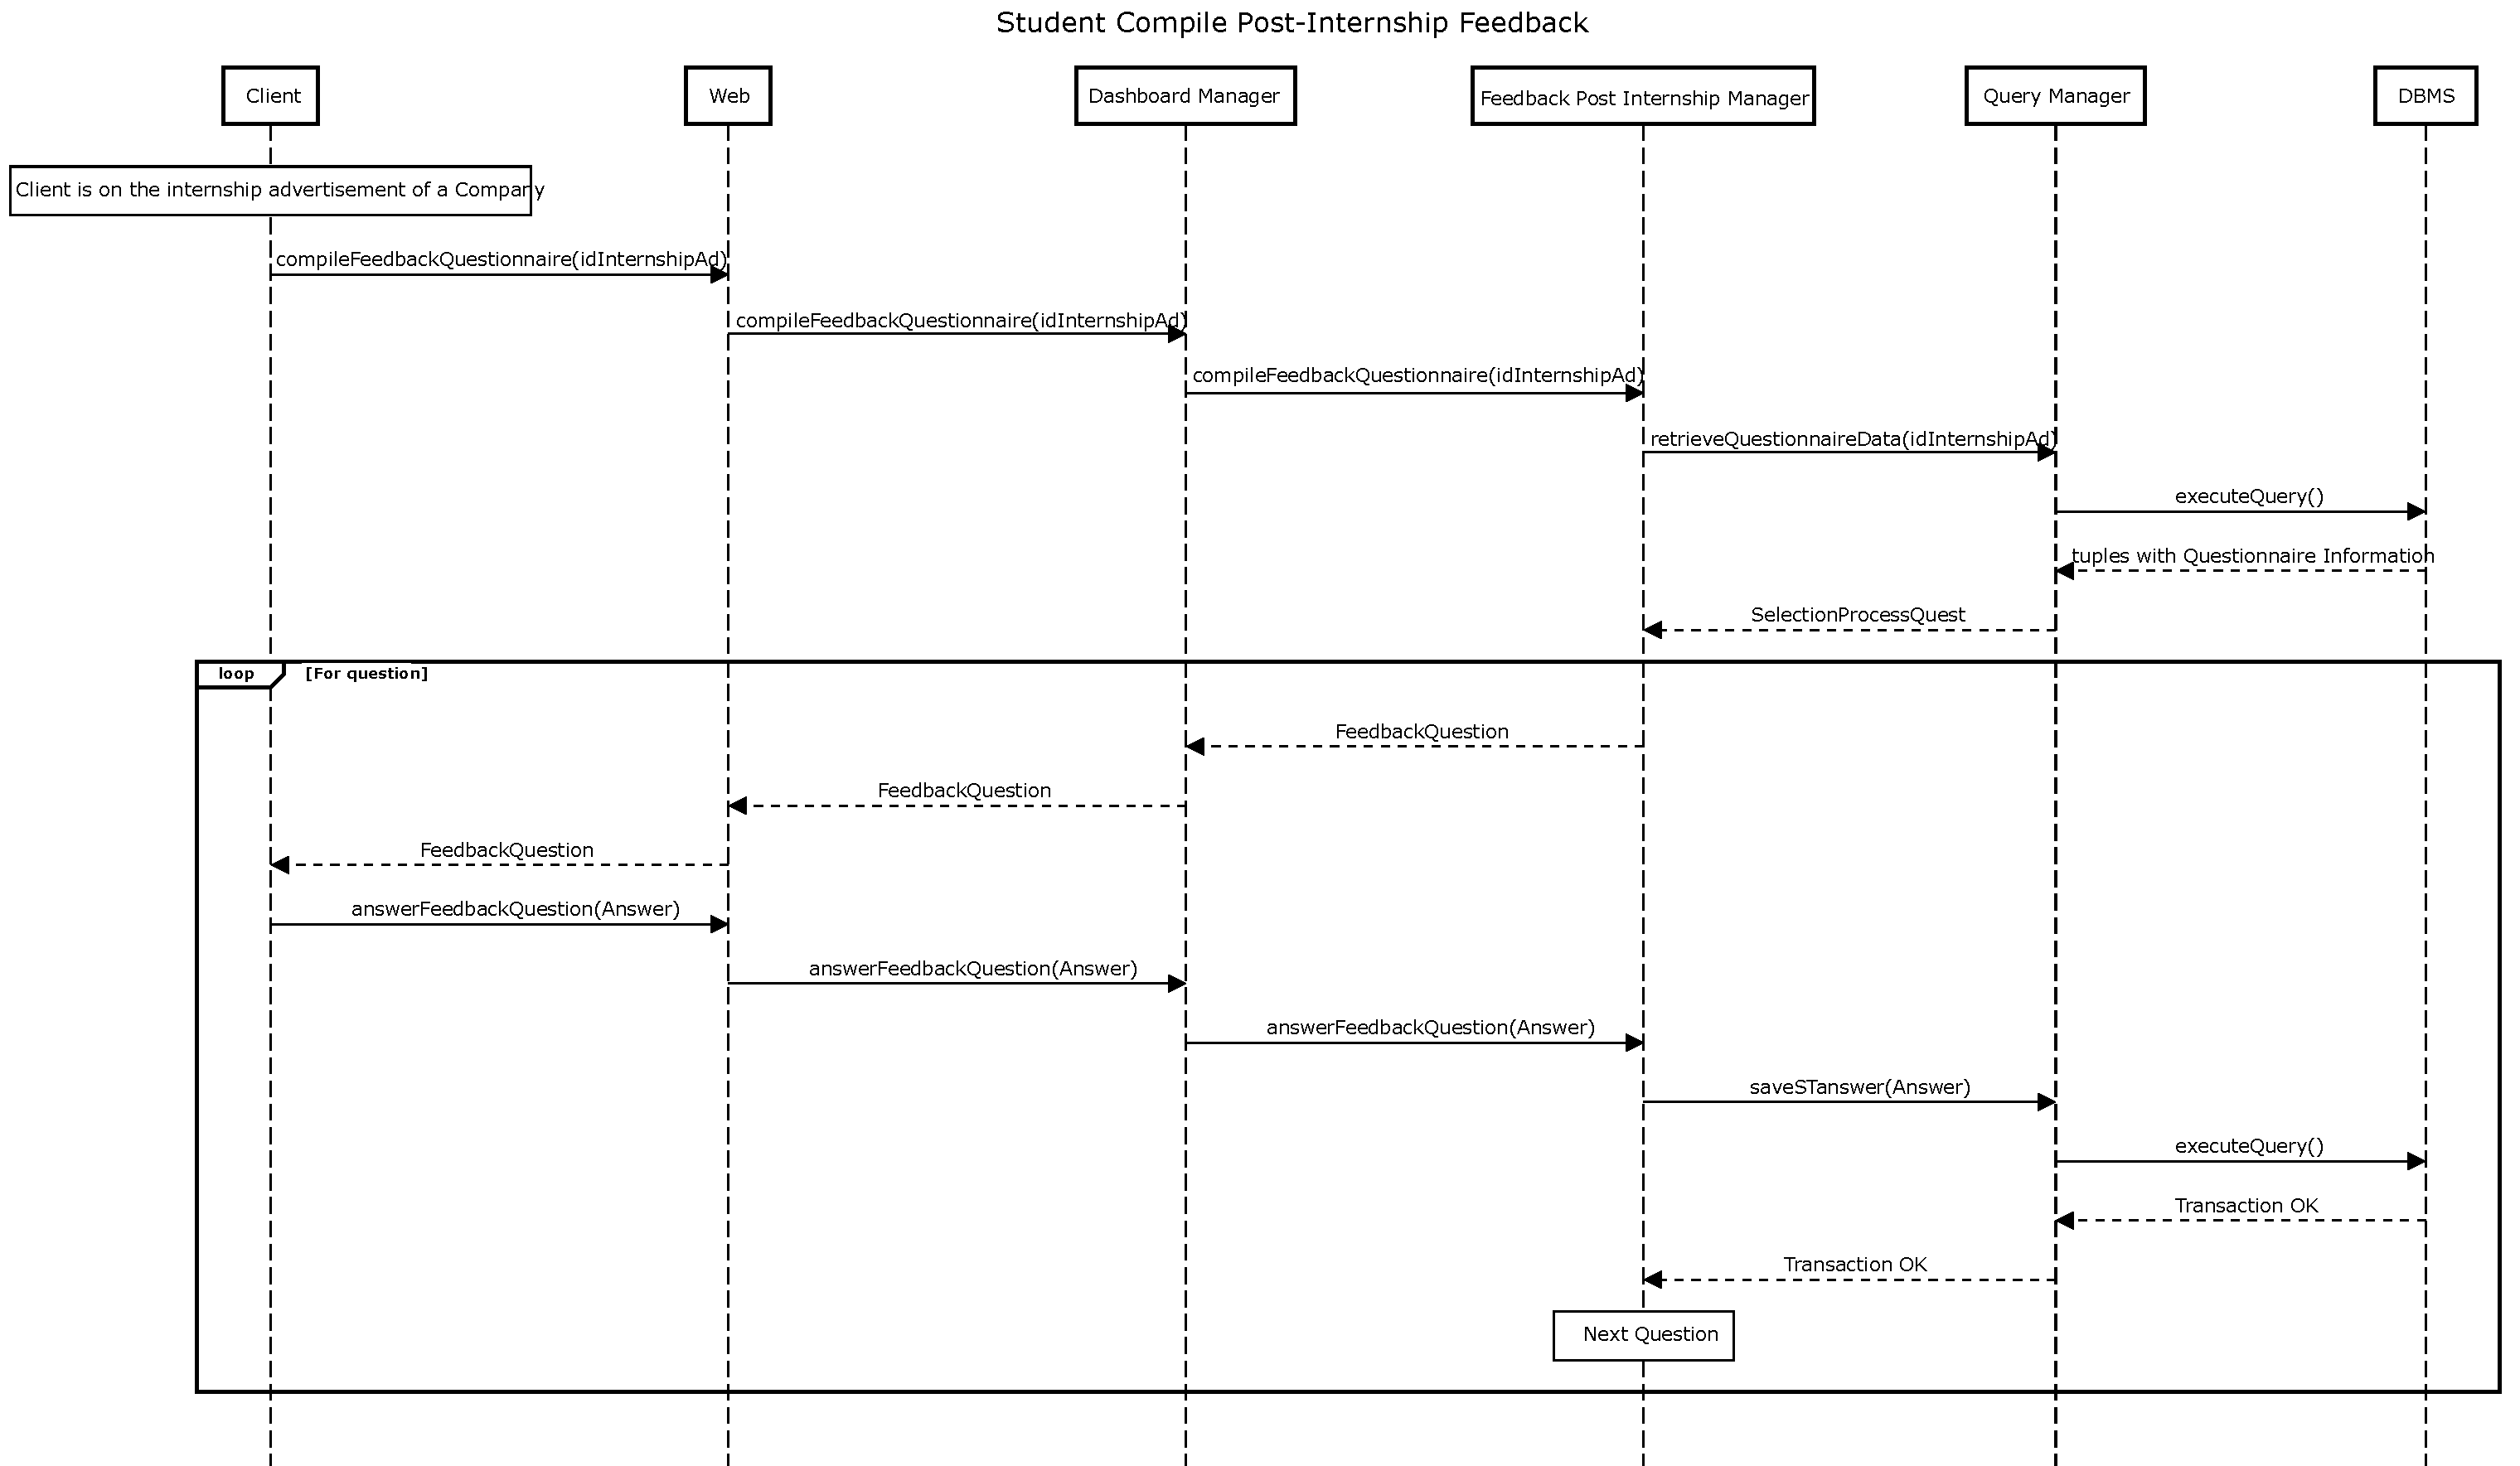
\includegraphics[width=0.85\textwidth]{Images/RV_04b.pdf}
      \caption{Runtime View - Student compiles Feedback Questionnaire}
      \label{fig:rv-student-compiles-feedback-questionnaire}
\end{figure}

\par This sequence diagram represents the ST compiles Feedback Questionnaire process. ST after receiving the email that
a feedback questionnaire for an internship he completed is available, To compile the questionnaire ST access the specified internship
advertisements and then clicks on the "Fill out Questionnaire" button or can directly access the questionnaire from the email.
In this case there is no deadline check because the questionnaire is for statistic and feedback purposes. The S\&C server retrieves
through the Feedback Questionnaire Manager the questions of the questionnaire and sends them one by one to the ST.
The ST answers the questions and clicks on the "Next" button. The S\&C server saves the answers and sends the next question
until the last one.

\subsection{Student creates a complaint}
\label{sub:student-creates-a-complaint}%

\begin{figure}[H]
      \centering
      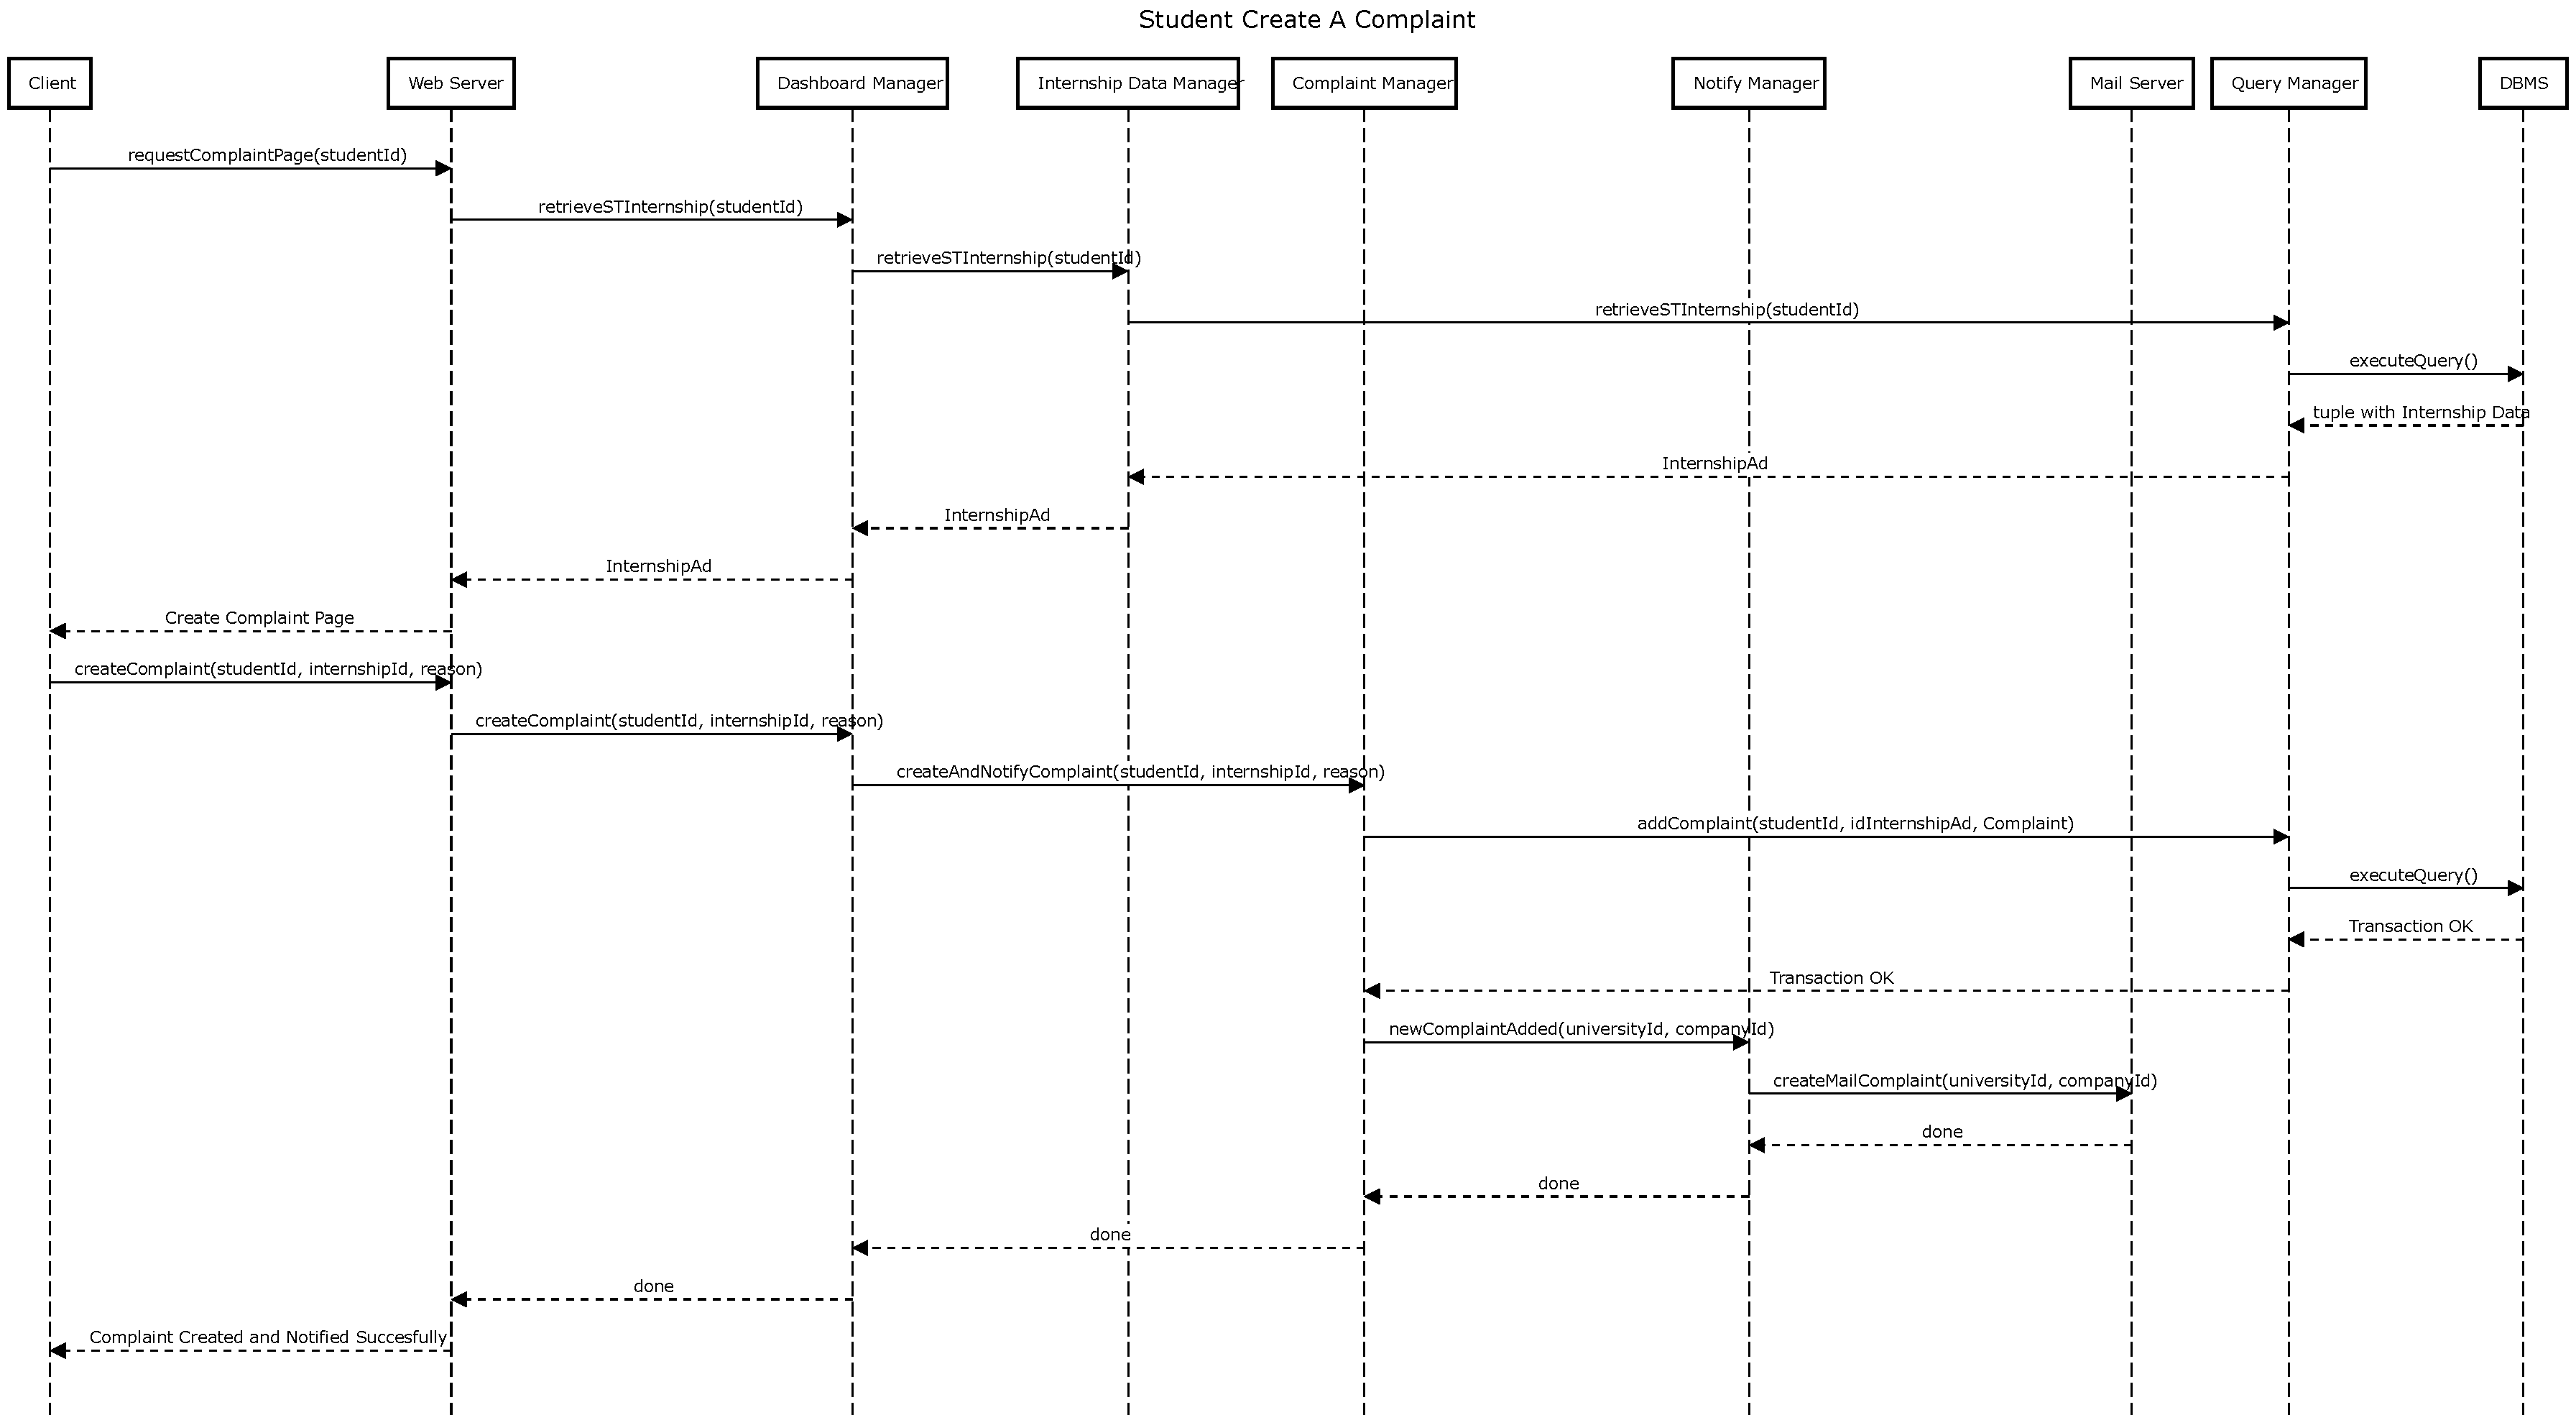
\includegraphics[width=0.85\textwidth]{Images/RV_05.pdf}
      \caption{Runtime View - Student creates a complaint}
      \label{fig:rv-student-creates-a-complaint}
\end{figure}

\par This sequence diagram represents the ST creates a complaint process. ST clicks on the "Create Complaint" button in the
dashboard page. The S\&C server sends back the complaint creation page after retrieving the internships that the ST is involved in,
if the ST is not involved in any internship the page will show that a complaint can't be created. The ST selects the internship
and the reason for the complaint and writes the complaint in the text area. The ST clicks on the "Submit" button. The S\&C server
saves the complaint and sends a notification to the CO and UN staff involved in the internship.

\subsection{Company creates an internship advertisement}
\label{sub:company-creates-an-internship-advertisement}%

\begin{figure}[H]
      \centering
      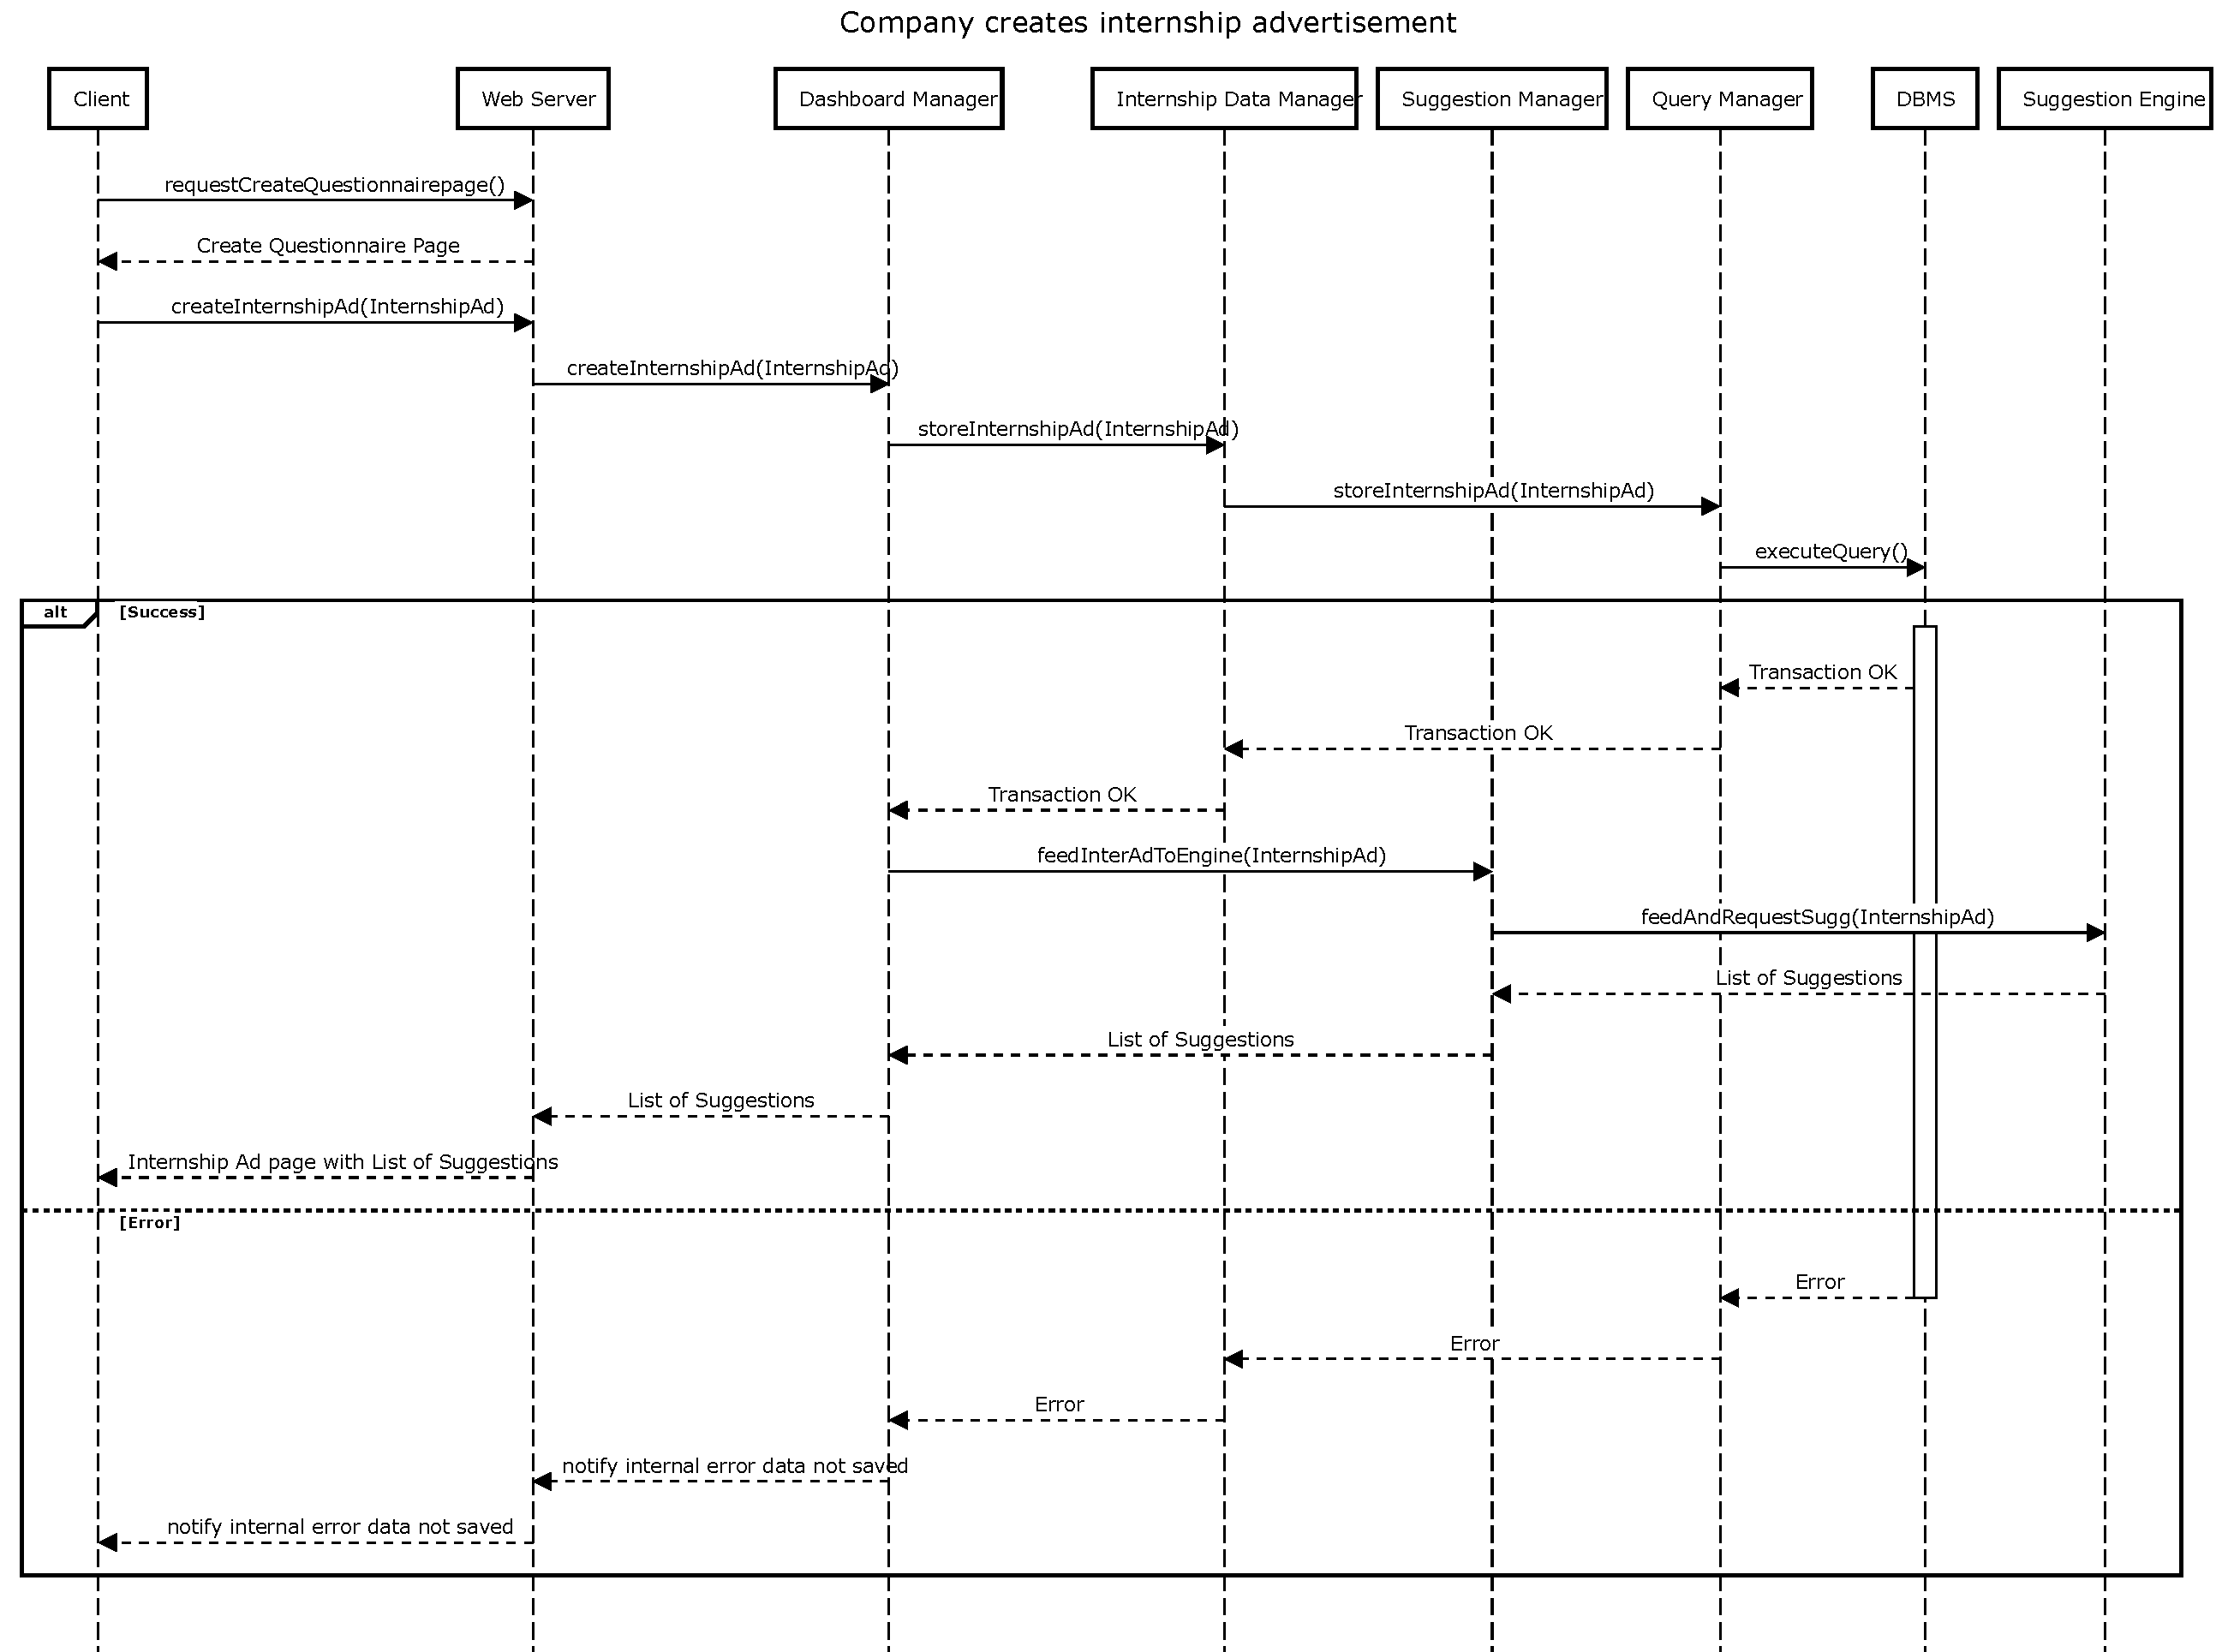
\includegraphics[width=0.85\textwidth]{Images/RV_06.pdf}
      \caption{Runtime View - Company creates an internship advertisement}
      \label{fig:rv-company-creates-an-internship-advertisement}
\end{figure}

\par This sequence diagram represents the CO creates an internship advertisement process. CO clicks on the "Create Internship
Advertisement" button in the dashboard page. The S\&C server sends back the internship advertisement creation page. The CO fills
the form with the details of the internship advertisement and clicks on the "Submit" button. If the internship advertisement is
saved correctly then the S\&C server feeds the data to the Suggestion Engine to be analyzed and suggestions are sent back to the CO.

% RV 07
\subsection{Company creates a questionnaire}
\label{sub:company-creates-a-questionnaire}%

\begin{figure}[H]
      \centering
      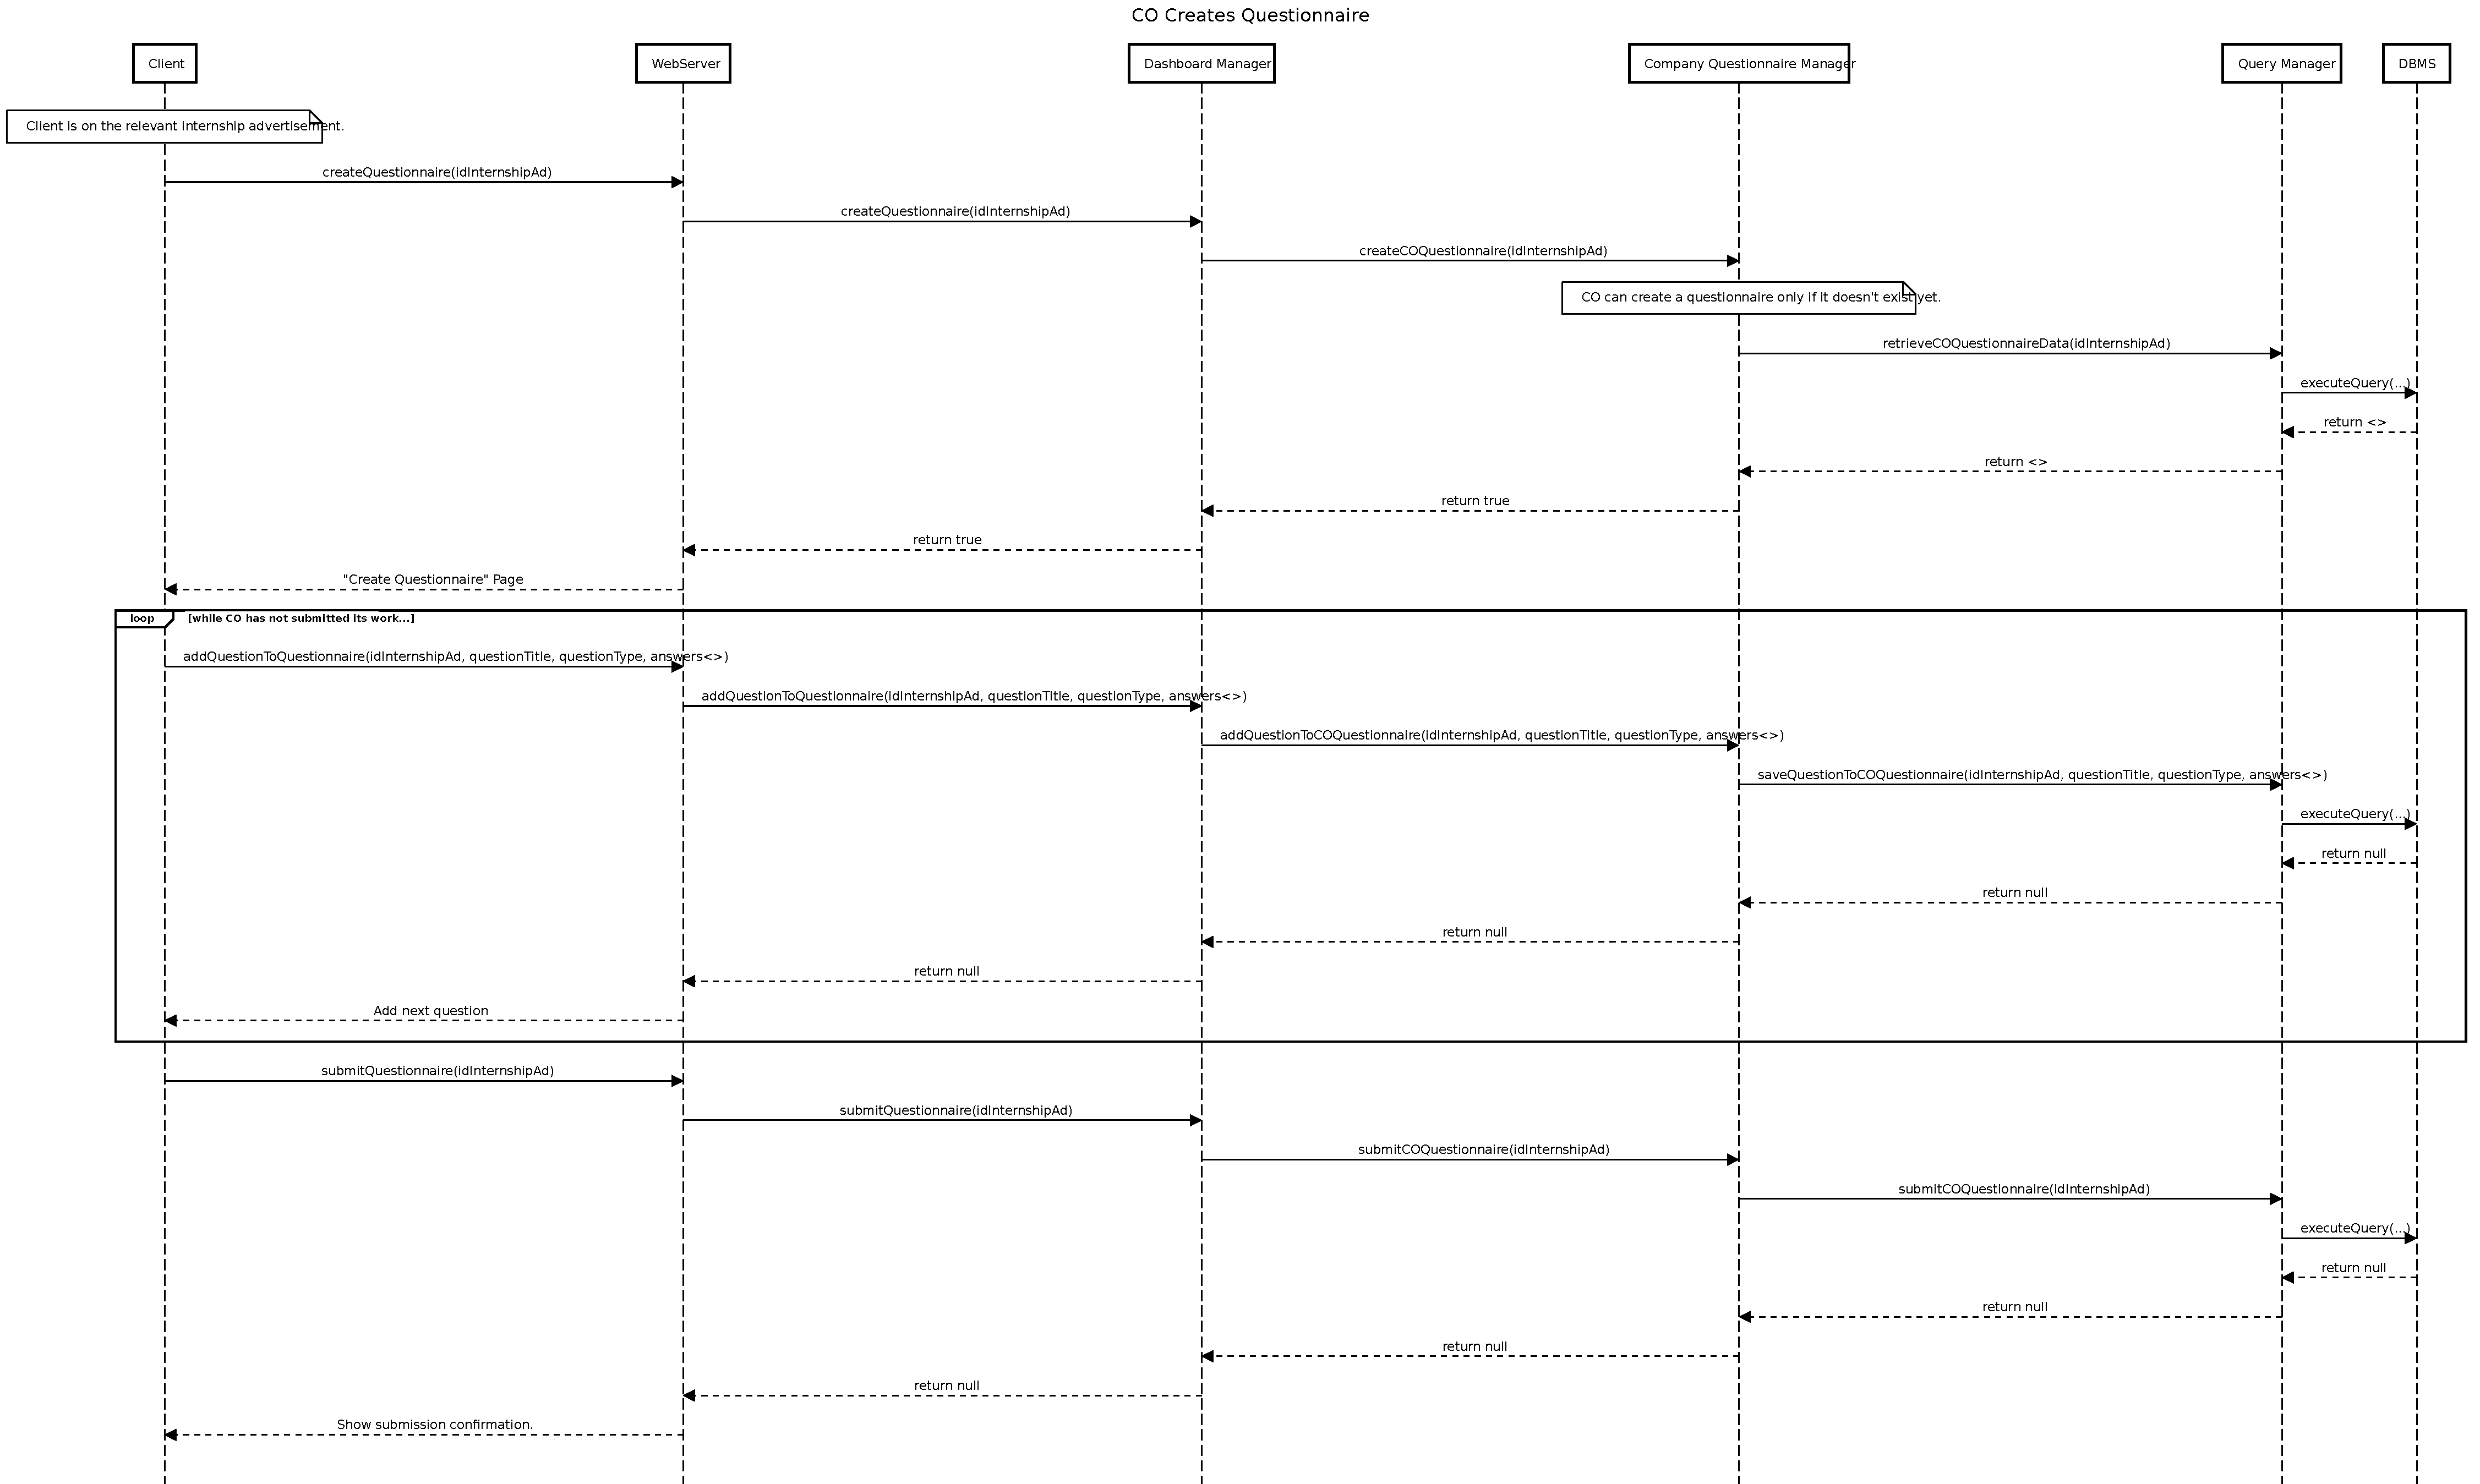
\includegraphics[width=1.0\textwidth]{Images/RV_07.pdf}
      \caption{Runtime View - Company creates a questionnaire for selecting students}
      \label{fig:rv-co-creates-questionnaire}
\end{figure}

\par This sequence diagram illustrates the general process involved by a CO in creating a questionnaire for selecting
and evaluating candidates for the relevant internship. The CO is viewing the internship advertisement and clicks on the
"Create Questionnaire" button. The S\&C server checks if a form has already been created for the that internship, and
if not, allows the client to open the questionnaire creation page. The CO then fills in the form with the questions
that they wish to ask the candidates and the points that each question is worth. Since the form that CO is creating
maybe long and complex, the client sends each question to the server as it is created. Once the form is completed, the
CO clicks on the "Submit" button. The S\&C server saves the form and sends a confirmation message to the CO.

% RV 08
\subsection{Company selects applicants to send questionnaire to}
\label{sub:company-selects-applicants-to-send-questionnaire-to}%

\begin{figure}[H]
      \centering
      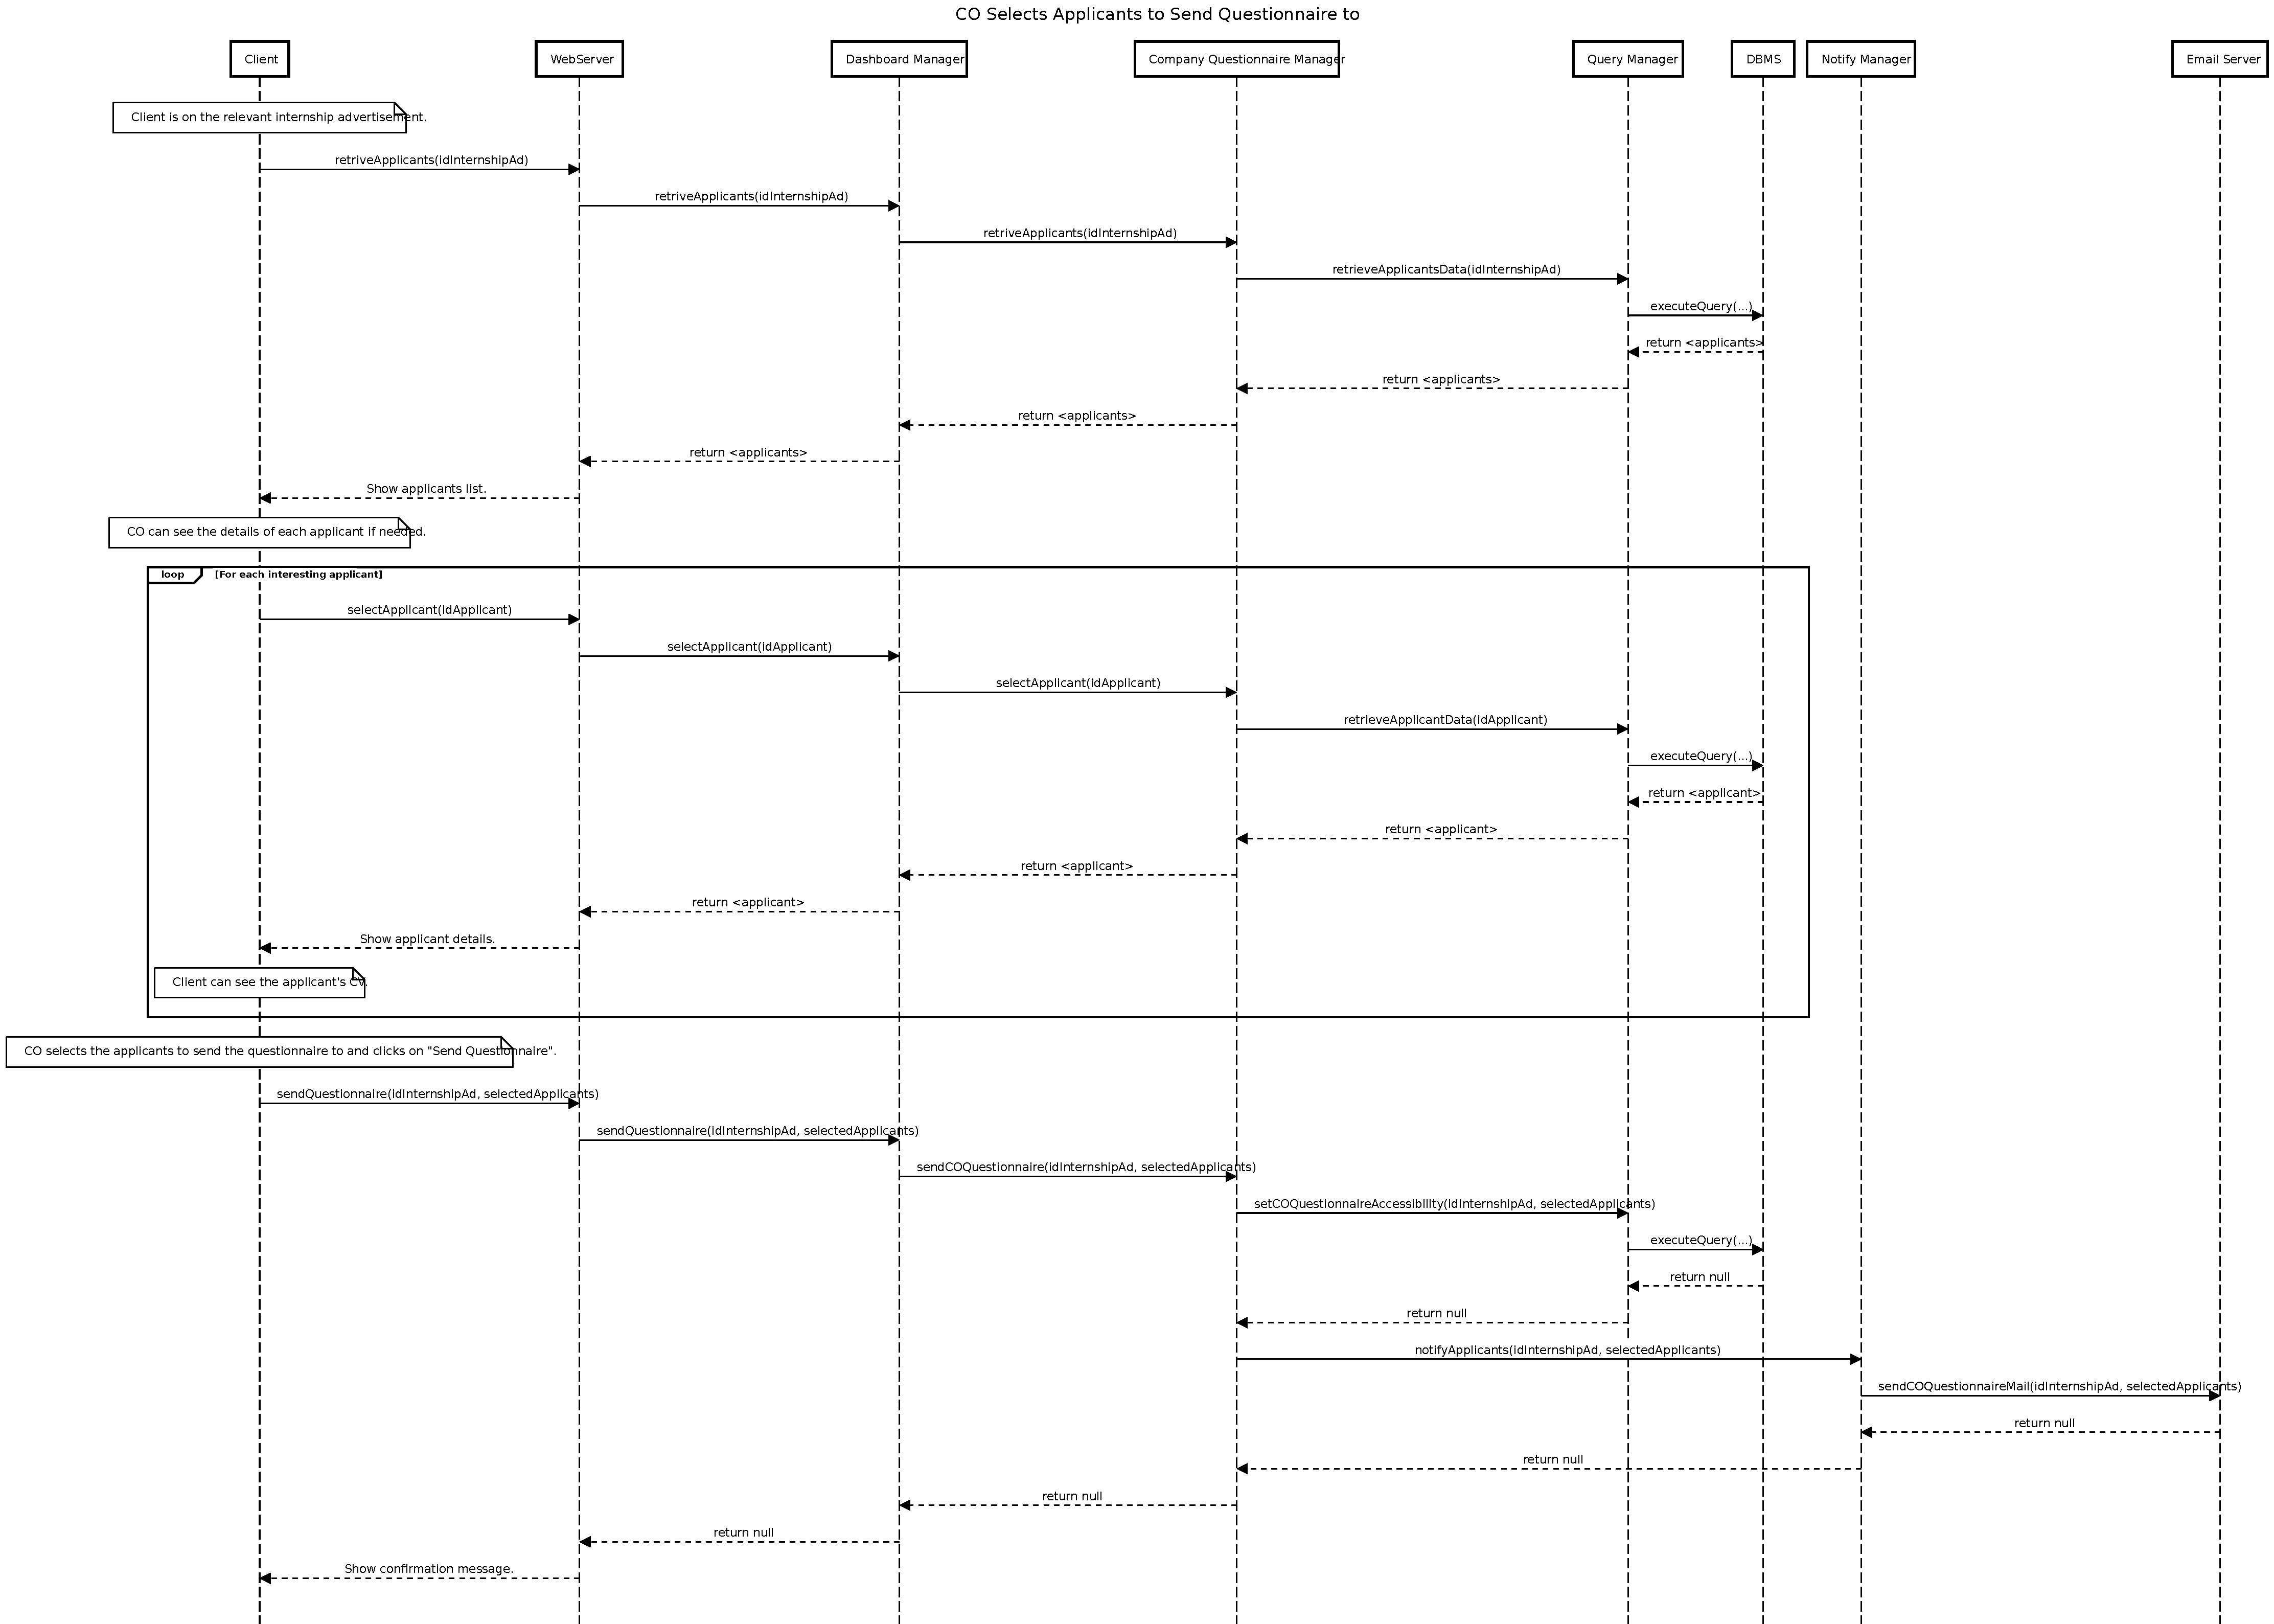
\includegraphics[width=1.0\textwidth]{Images/RV_08.pdf}
      \caption{Runtime View - Company selects applicants to send questionnaire to}
      \label{fig:rv-co-selects-applicants}
\end{figure}

\par This sequence diagram illustrates the process involved by a CO in selecting applicants to send a questionnaire to
for the relevant internship. The CO is viewing the internship advertisement and clicks on the "Send Questionnaire"
button. The S\&C server retrieves the list of applicants for the internship and sends it to the client that will
displays it. If the CO wishes so they can see the profile of each applicant individually in order to make a more
informed decision. The CO then selects all the applicants that they wish to send the questionnaire to and clicks on
the "Send" button. The candidates pool is identified and sent to the S\&C server. S\&C Core will then notify all
selected students via email - using the Email Server - that they have a questionnaire to fill out.

% RV 09
\subsection{Company edits its own profile}
\label{sub:company-edits-its-own-profile}%

\begin{figure}[H]
      \centering
      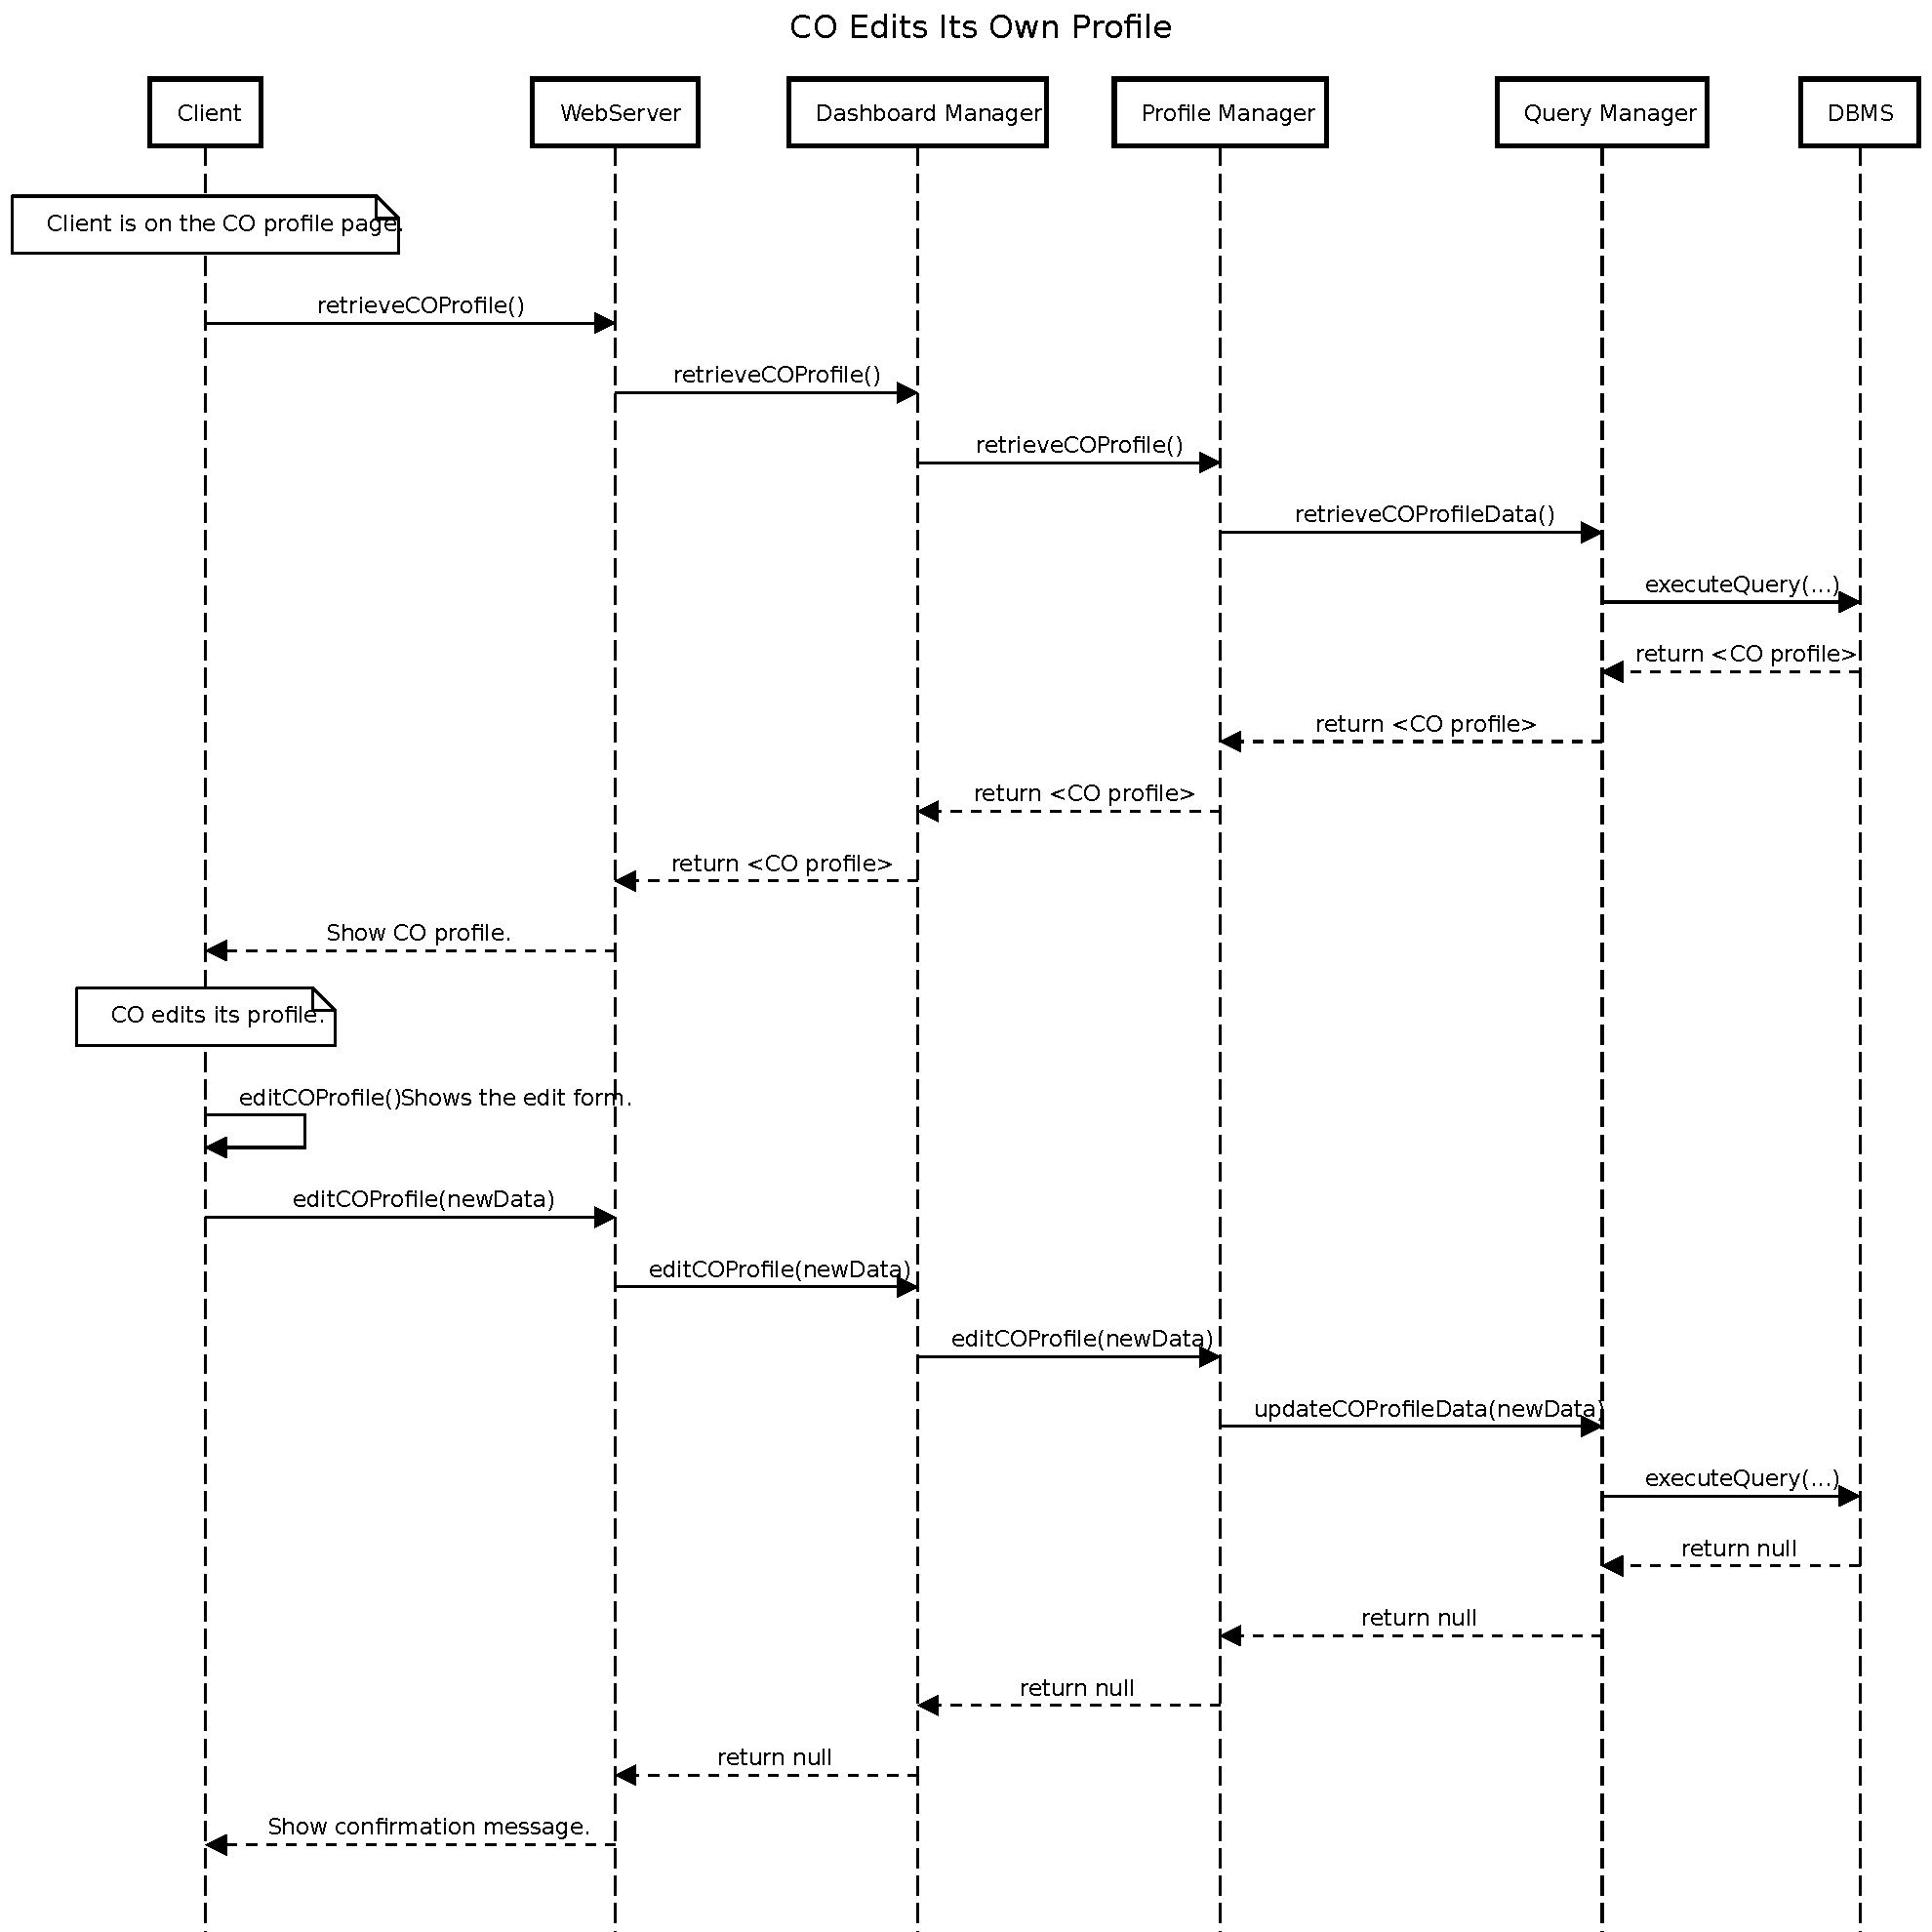
\includegraphics[width=1.0\textwidth]{Images/RV_09.pdf}
      \caption{Runtime View - Company edits its own profile}
      \label{fig:rv-co-edits-profile}
\end{figure}

\par This sequence diagram states how a CO can edit its own profile page. The CO clicks on the "Edit Profile" button
in its own profile page. The client will than show the editing form. After the CO has made the necessary changes,
they click on the "Submit" button. The S\&C server will then save the changes and shows a confirmation message to the
CO.

% RV 10
\subsection{Company compiles the post-internship feedback form}
\label{sub:company-compiles-the-post-internship-feedback-form}%

\begin{figure}[H]
      \centering
      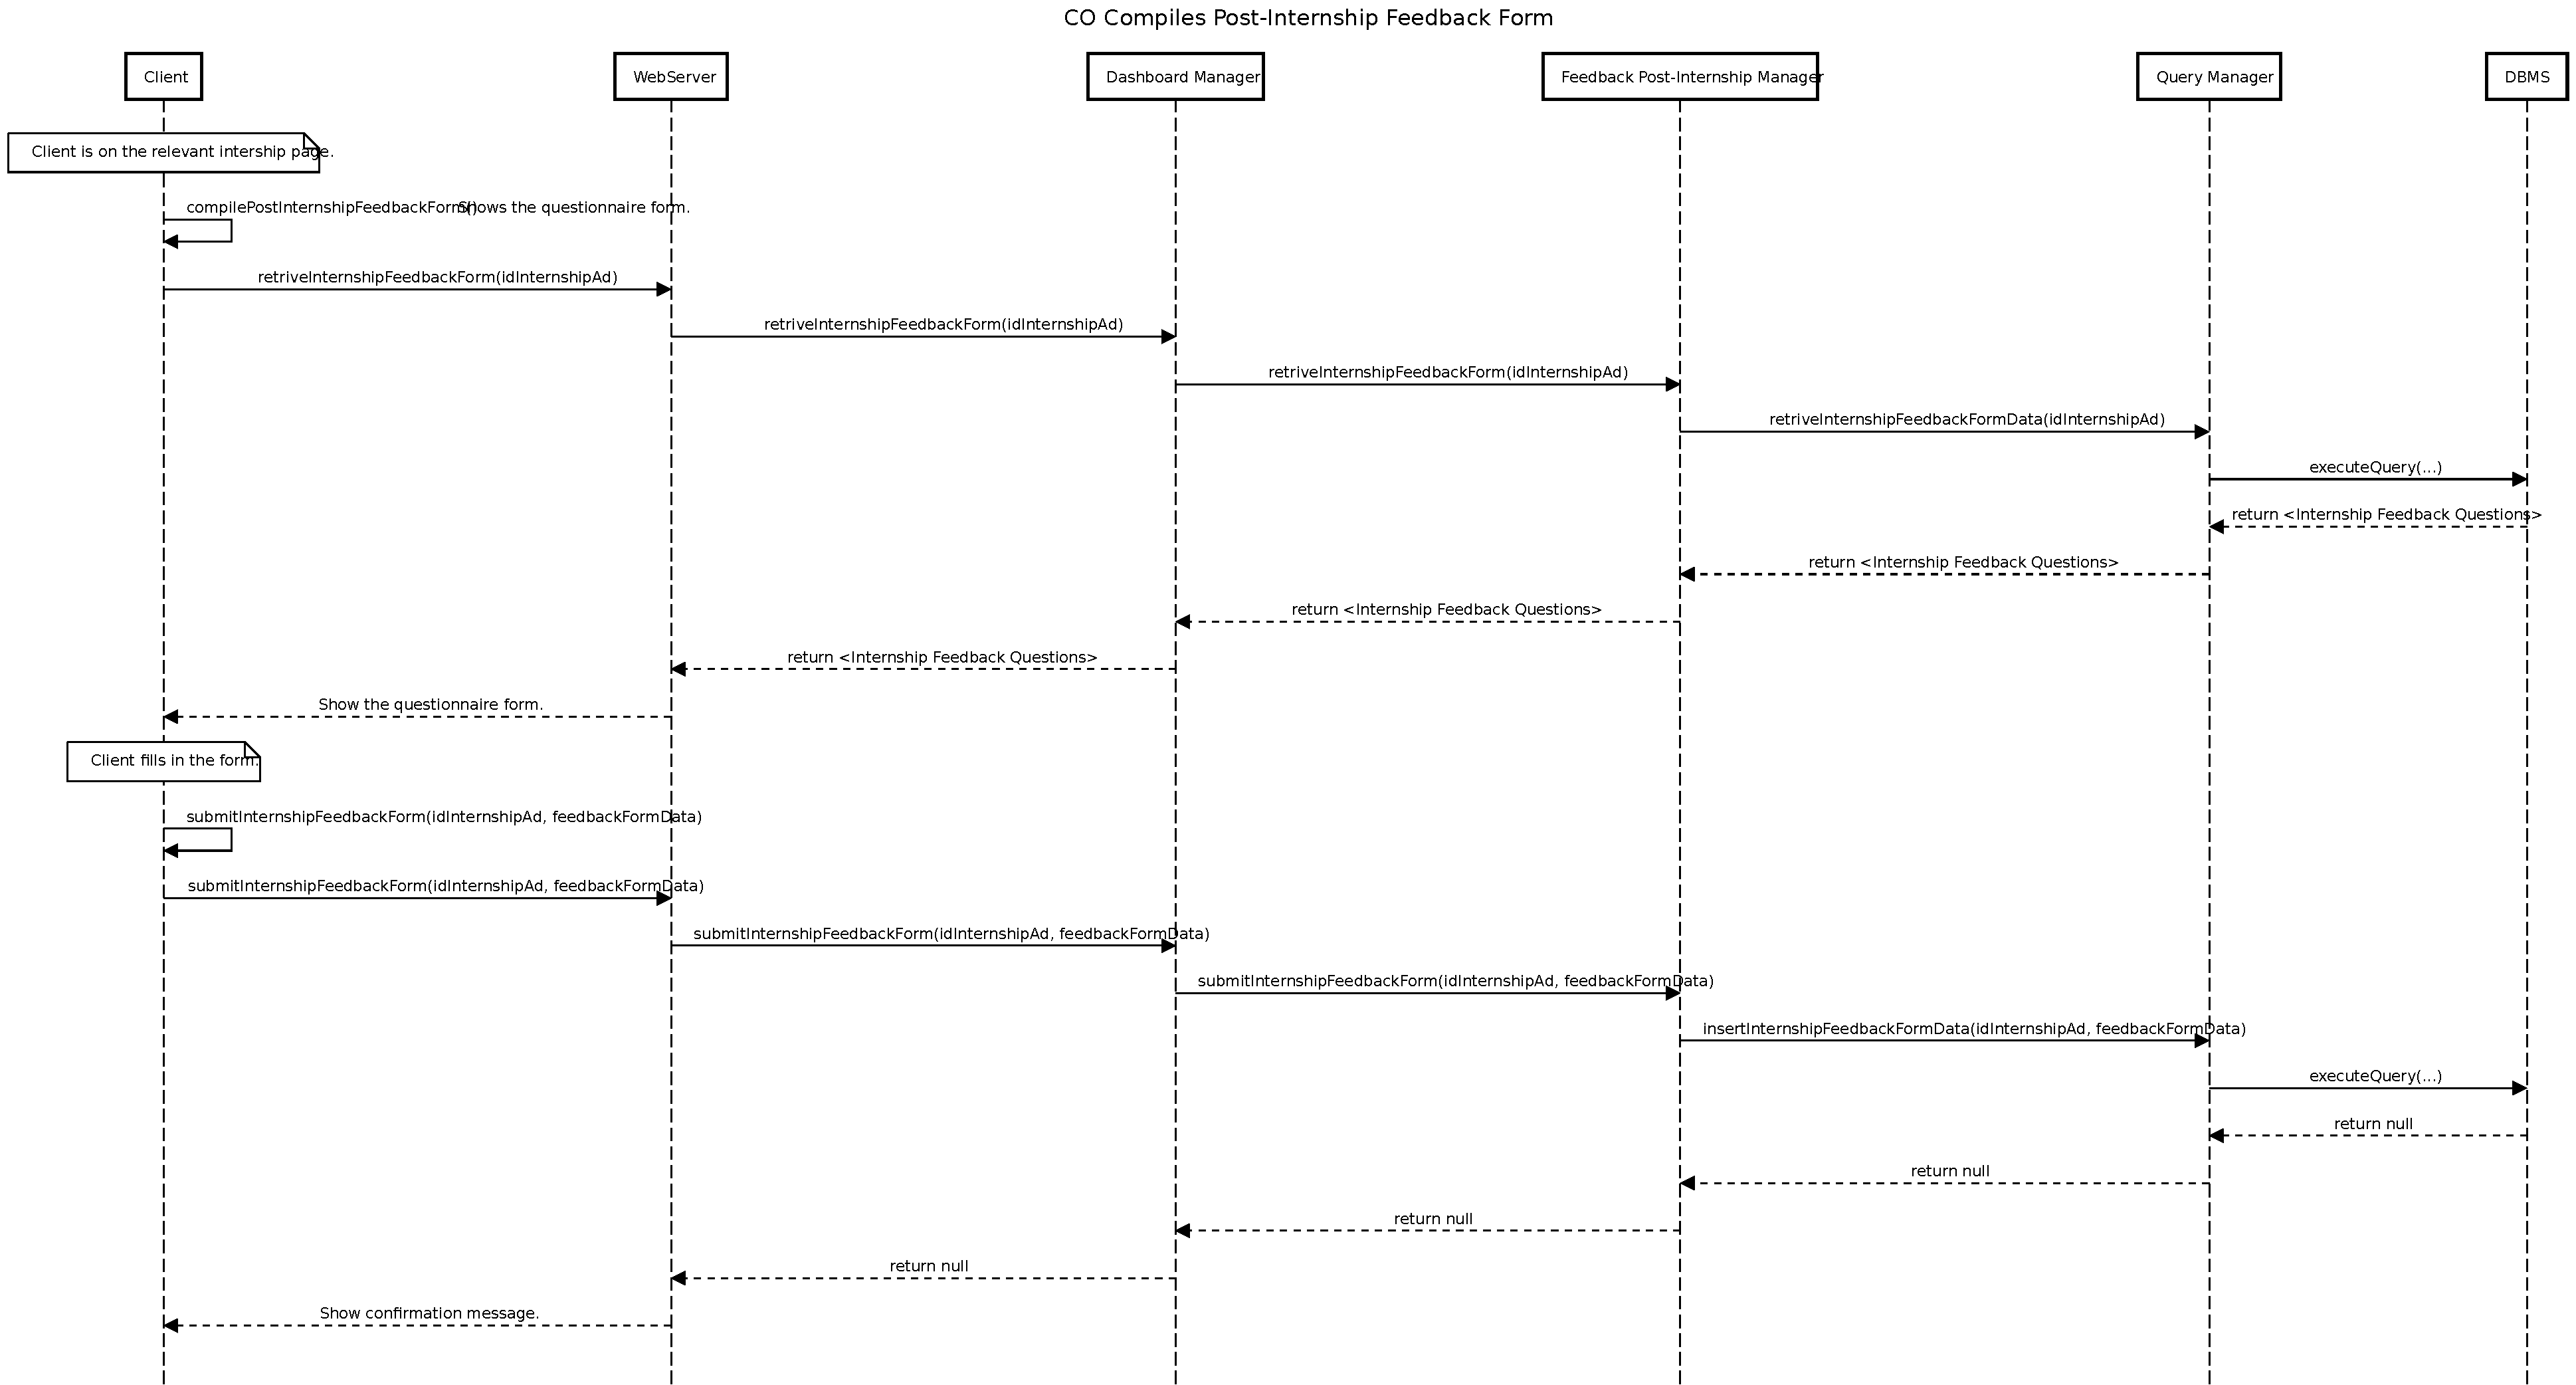
\includegraphics[width=1.0\textwidth]{Images/RV_10.pdf}
      \caption{Runtime View - Company compiles the post-internship feedback form}
      \label{fig:rv-co-compiles-feedback-form}
\end{figure}

\par This sequence diagram illustrates how the CO can compile the post-internship feedback form. The client is on the
now ended internship page and clicks on the "Post-Internship Feedback" button. The S\&C server retrieves the feedback
form and sends it to the client. The CO then fills in the form with the necessary information and clicks on the
"Submit" button. The S\&C server saves the feedback and sends a confirmation message to the CO.

\par Since this questionnaire are usually very short and simple, the client sends the entire form to the server at
once without saving the answers one by one.

% RV 11
\subsection{Company creates a complaint}
\label{sub:company-creates-a-complaint}%

\begin{figure}[H]
      \centering
      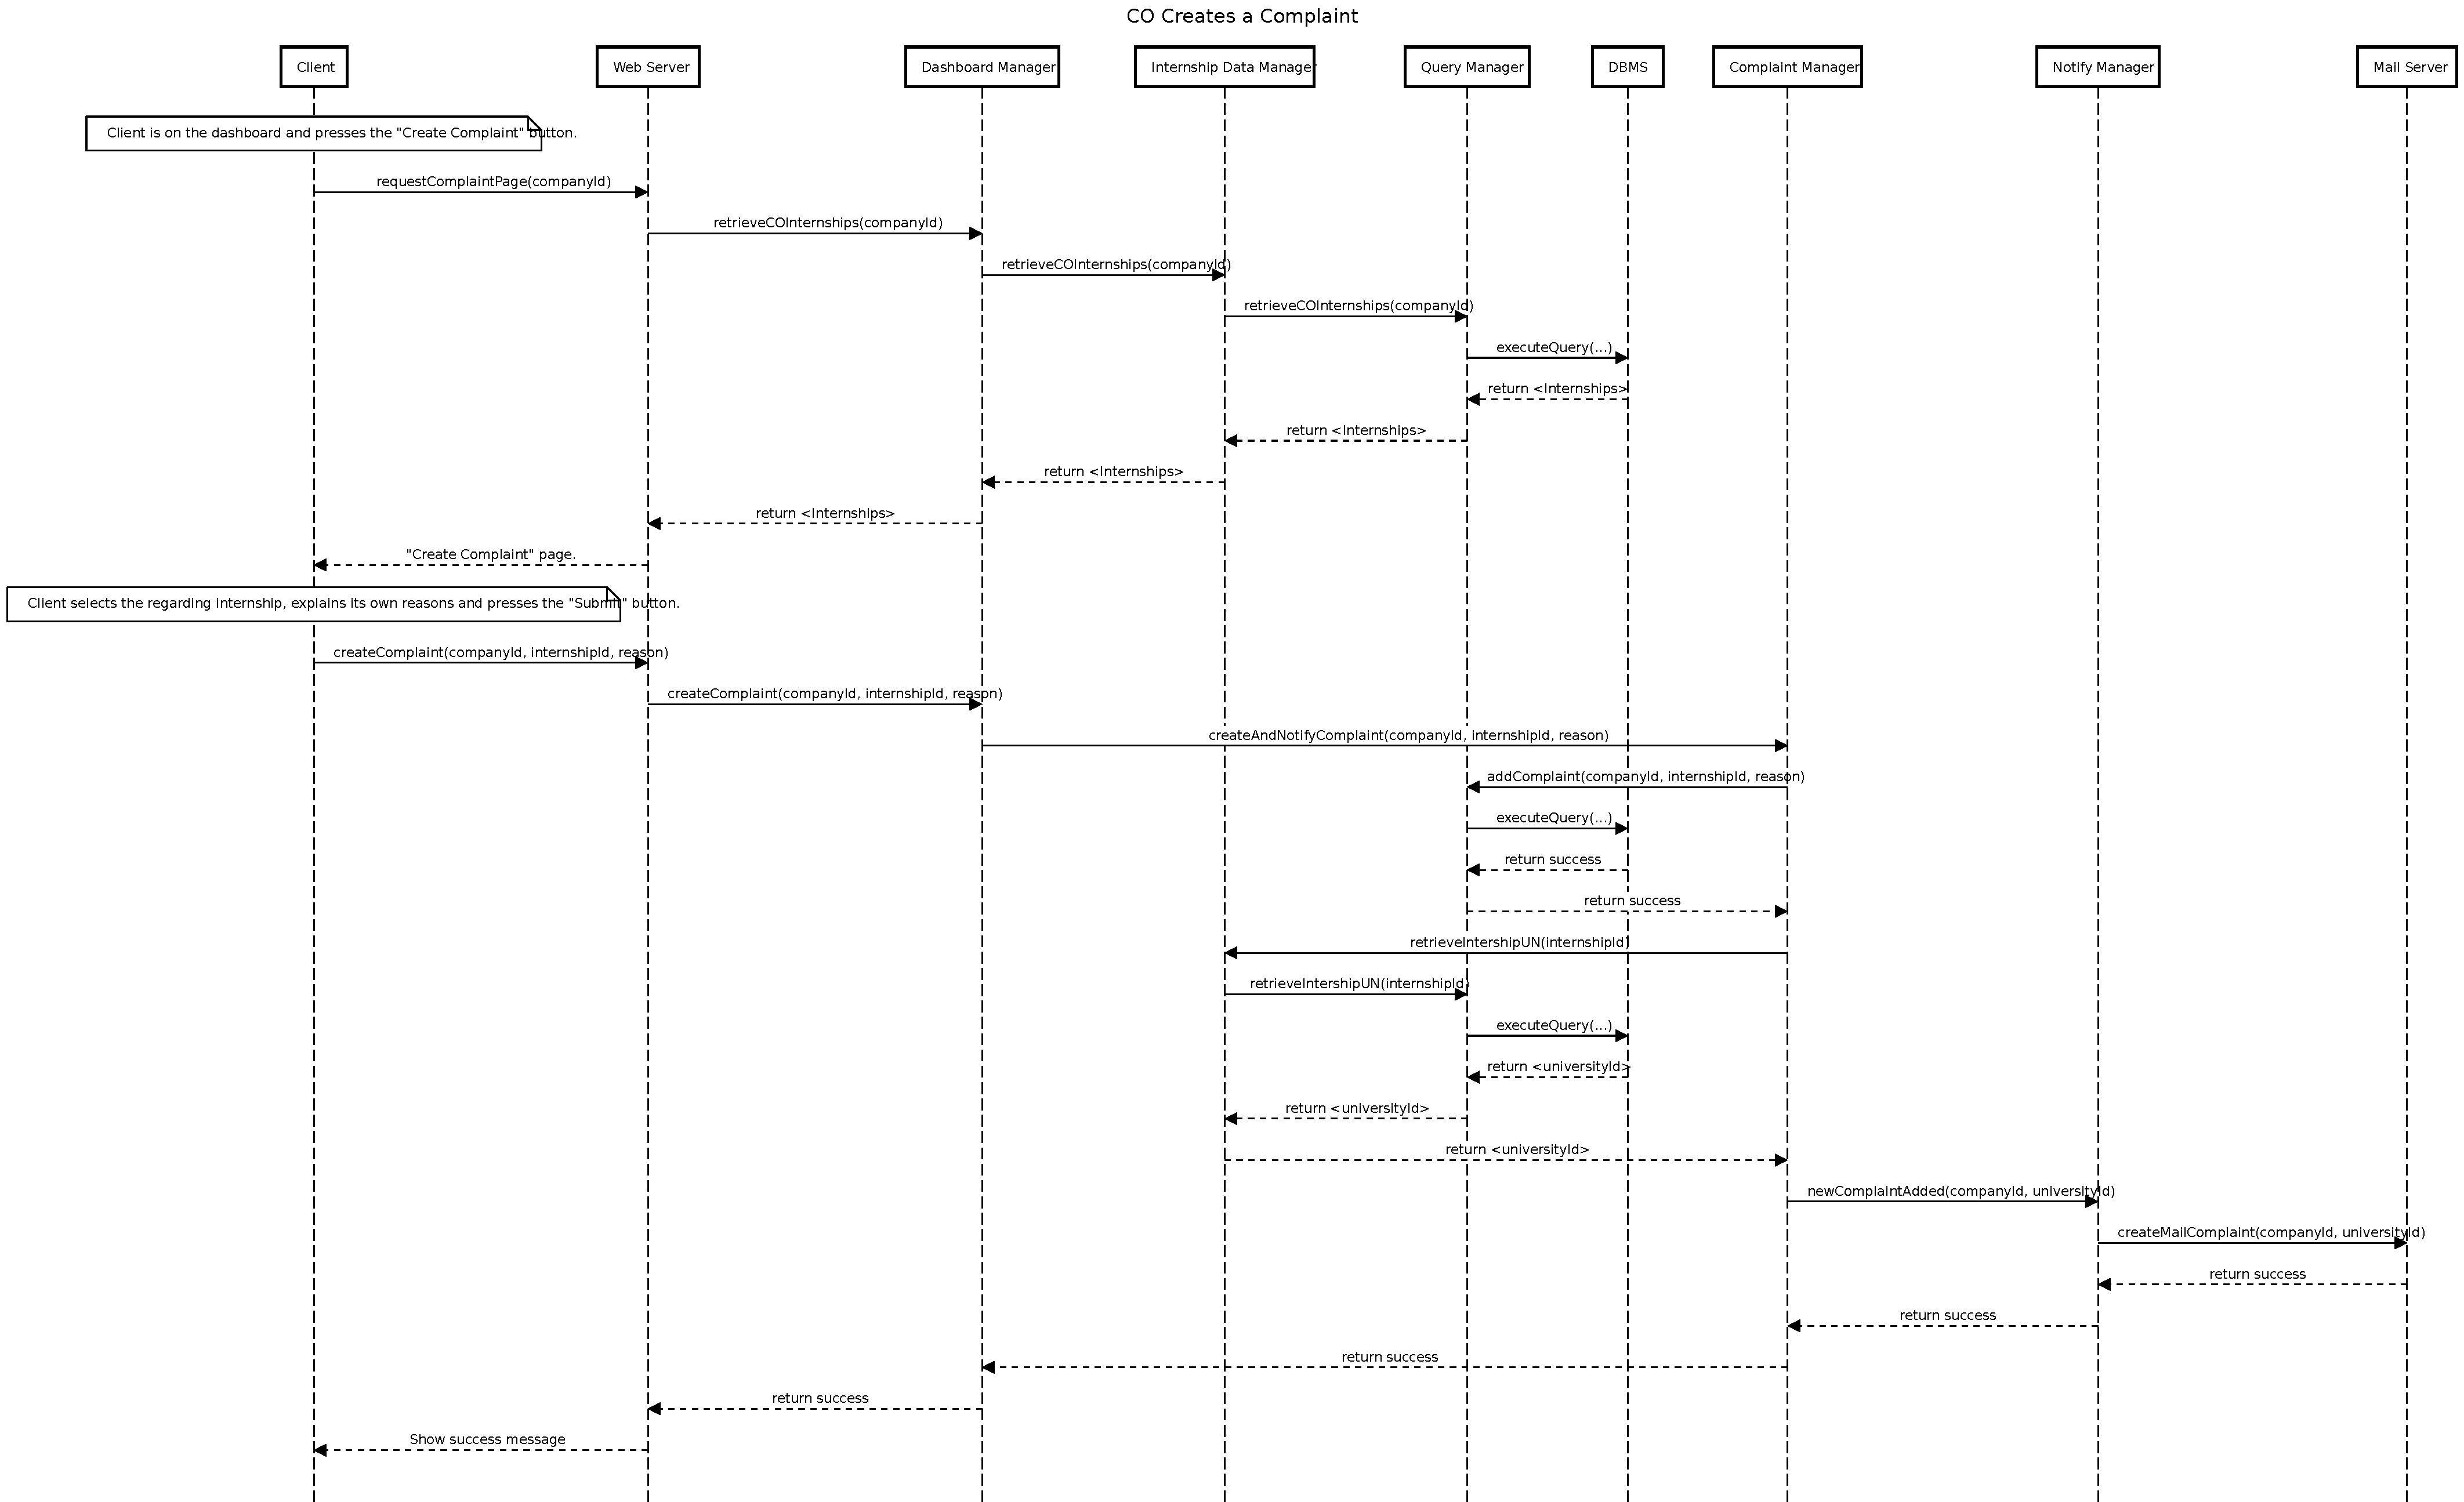
\includegraphics[width=1.0\textwidth]{Images/RV_11.pdf}
      \caption{Runtime View - Company creates a complaint}
      \label{fig:rv-co-creates-complaint}
\end{figure}

\par This sequence diagram illustrates how a CO can create a complaint. The client is on the dashboard and clicks
on the "Create Complaint" button. The S\&C server provides the client with the list of internships that the CO is
involved in to allow the CO to select the internship that the complaint is related to. The CO then writes the in the
form its reasons and clicks on the "Submit" button. The S\&C server saves the complaint and sends a notification to
the UN staff and the ST involved in the work experience.

\par Again, since the complaint form is short storing the intermediate answers is not necessary.

% RV 12
\subsection{University monitors the status of the internships}
\label{sub:university-monitors-the-status-of-the-internships}%

\begin{figure}[H]
      \centering
      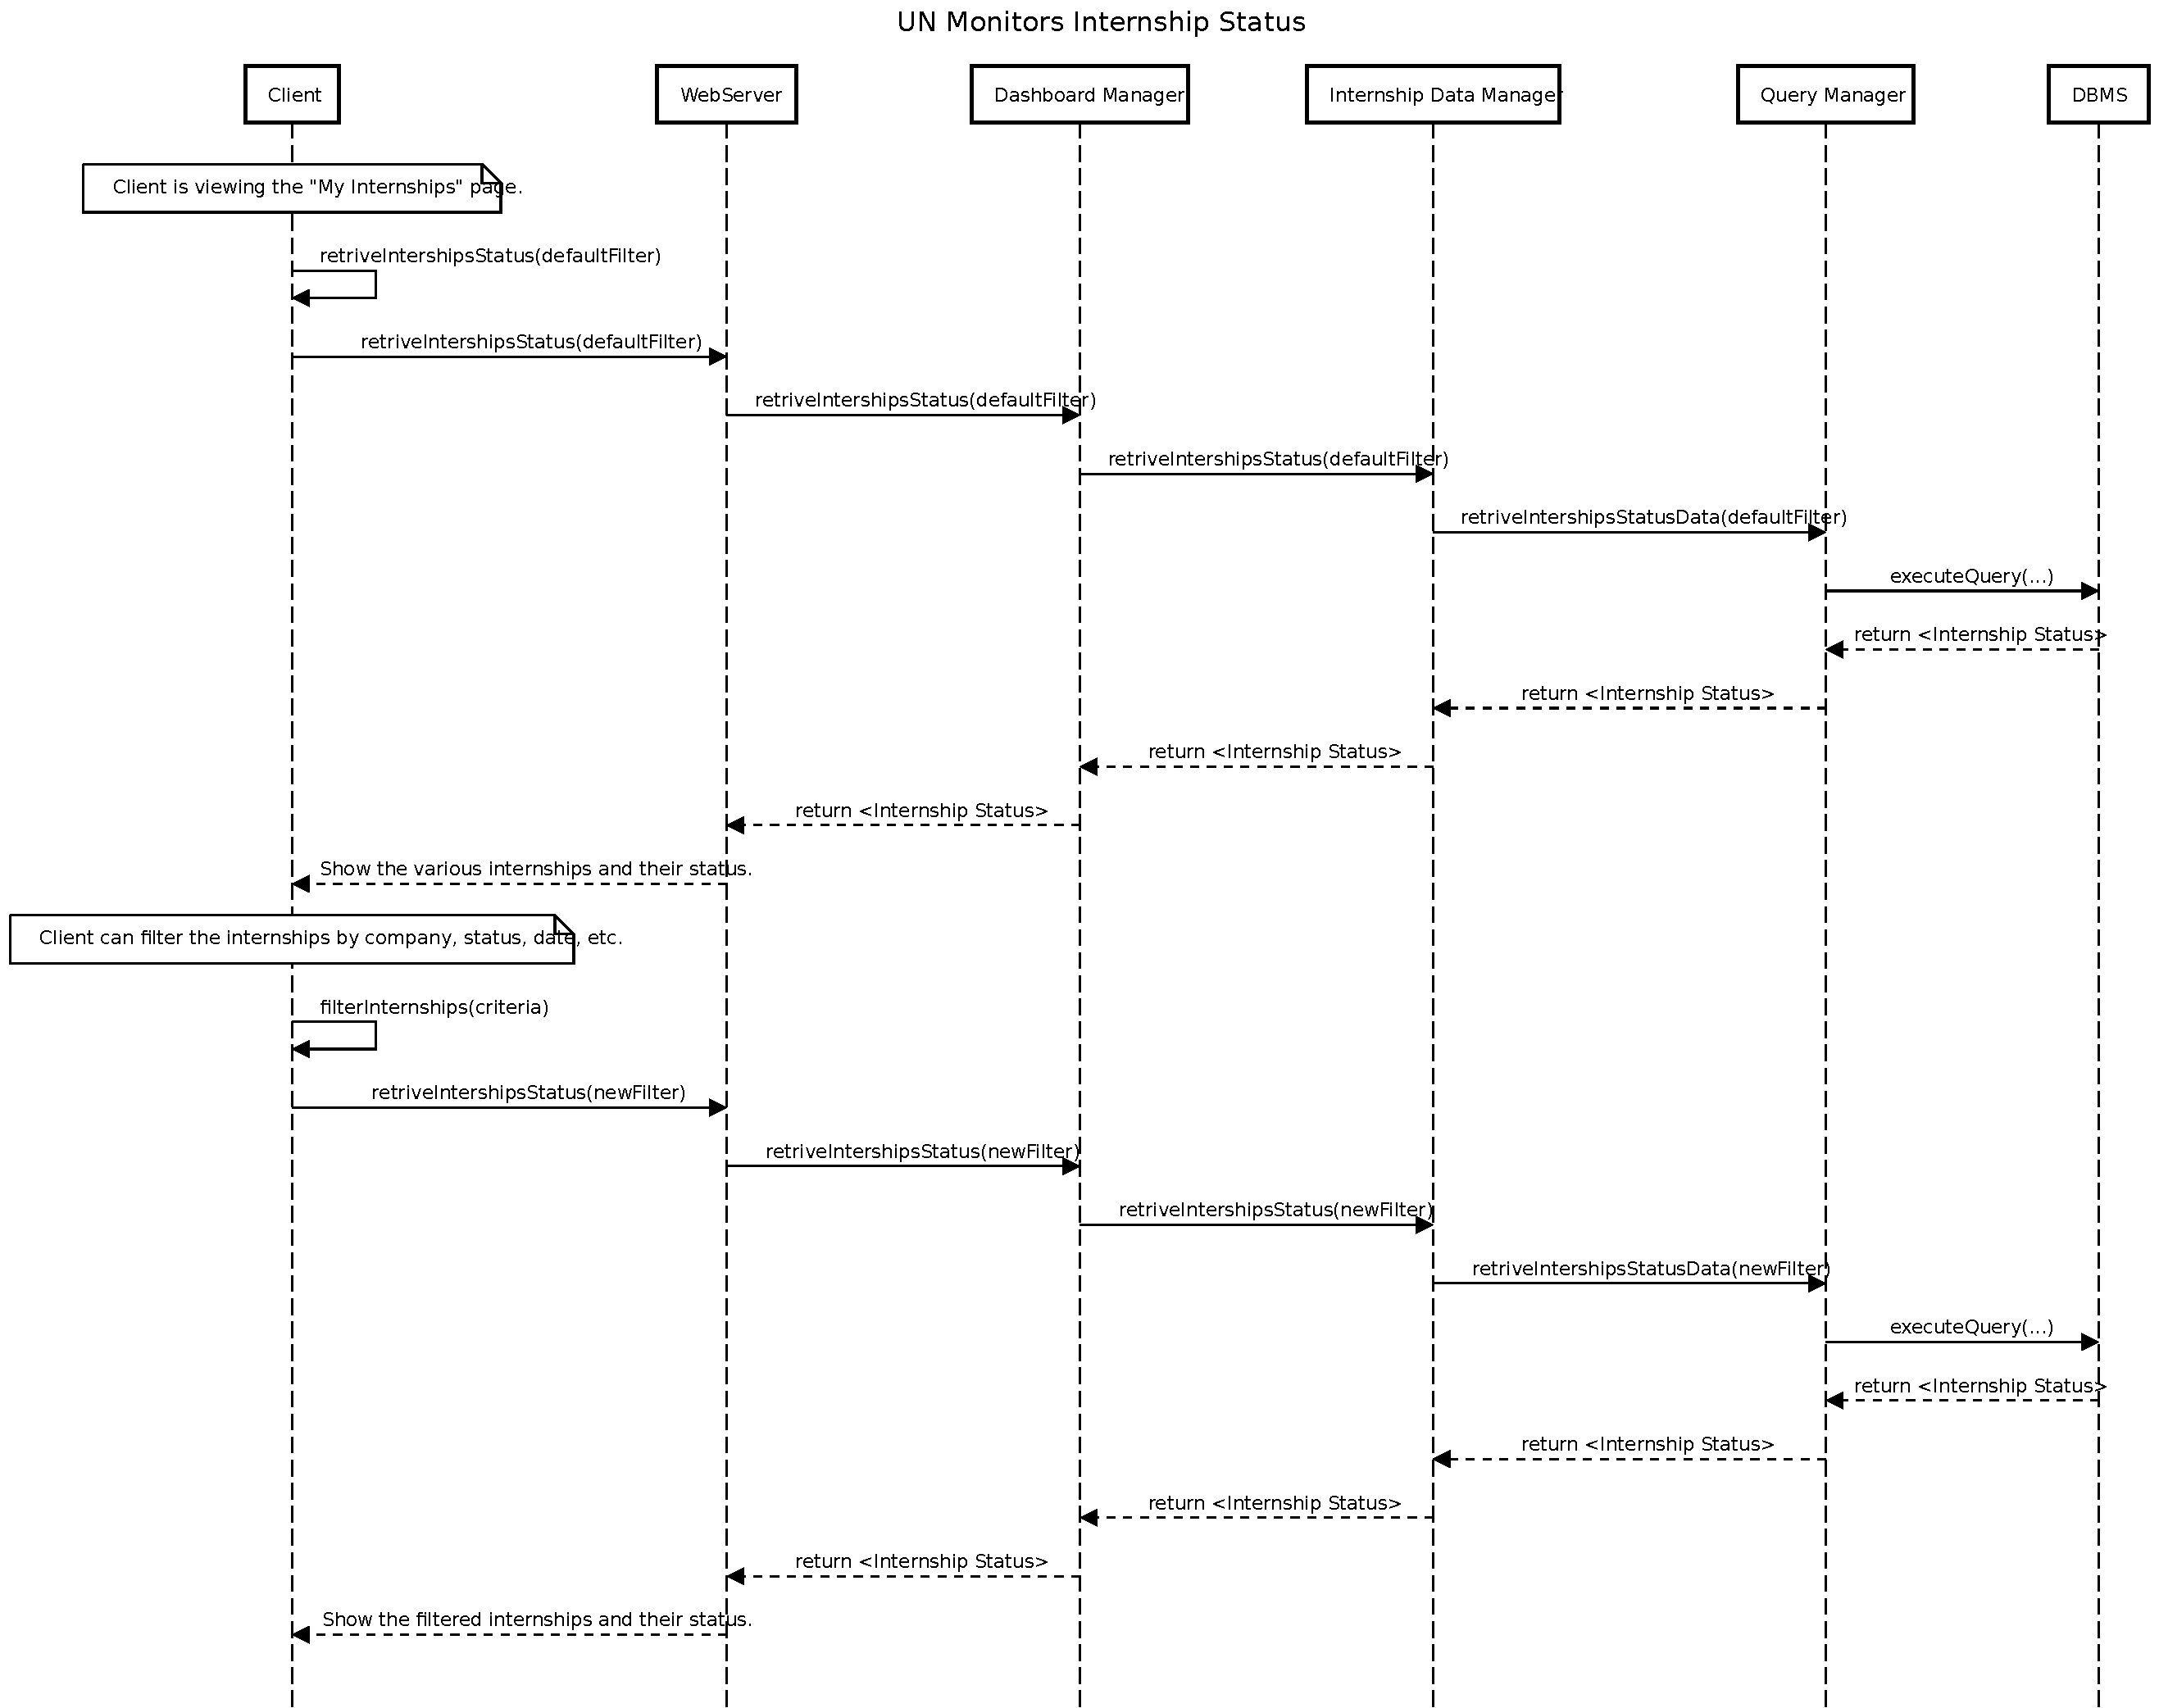
\includegraphics[width=1.0\textwidth]{Images/RV_12.pdf}
      \caption{Runtime View - University monitors the status of the internships}
      \label{fig:rv-un-monitors-internships}
\end{figure}

\par This sequence diagram illustrates how a UN can monitor the status of the internships. The clients load the "My
Internships" page. The S\&C server retrieves the list of internships that the UN is involved in and sends it to the
client. The UN can then see the status of each internship and if any complaints that have been made. If needed the UN
can filter the list by status, company, or other criteria to find the desired information.

% RV 13
\subsection{University handles a complaint}
\label{sub:university-handles-a-complaint}%

\begin{figure}[H]
      \centering
      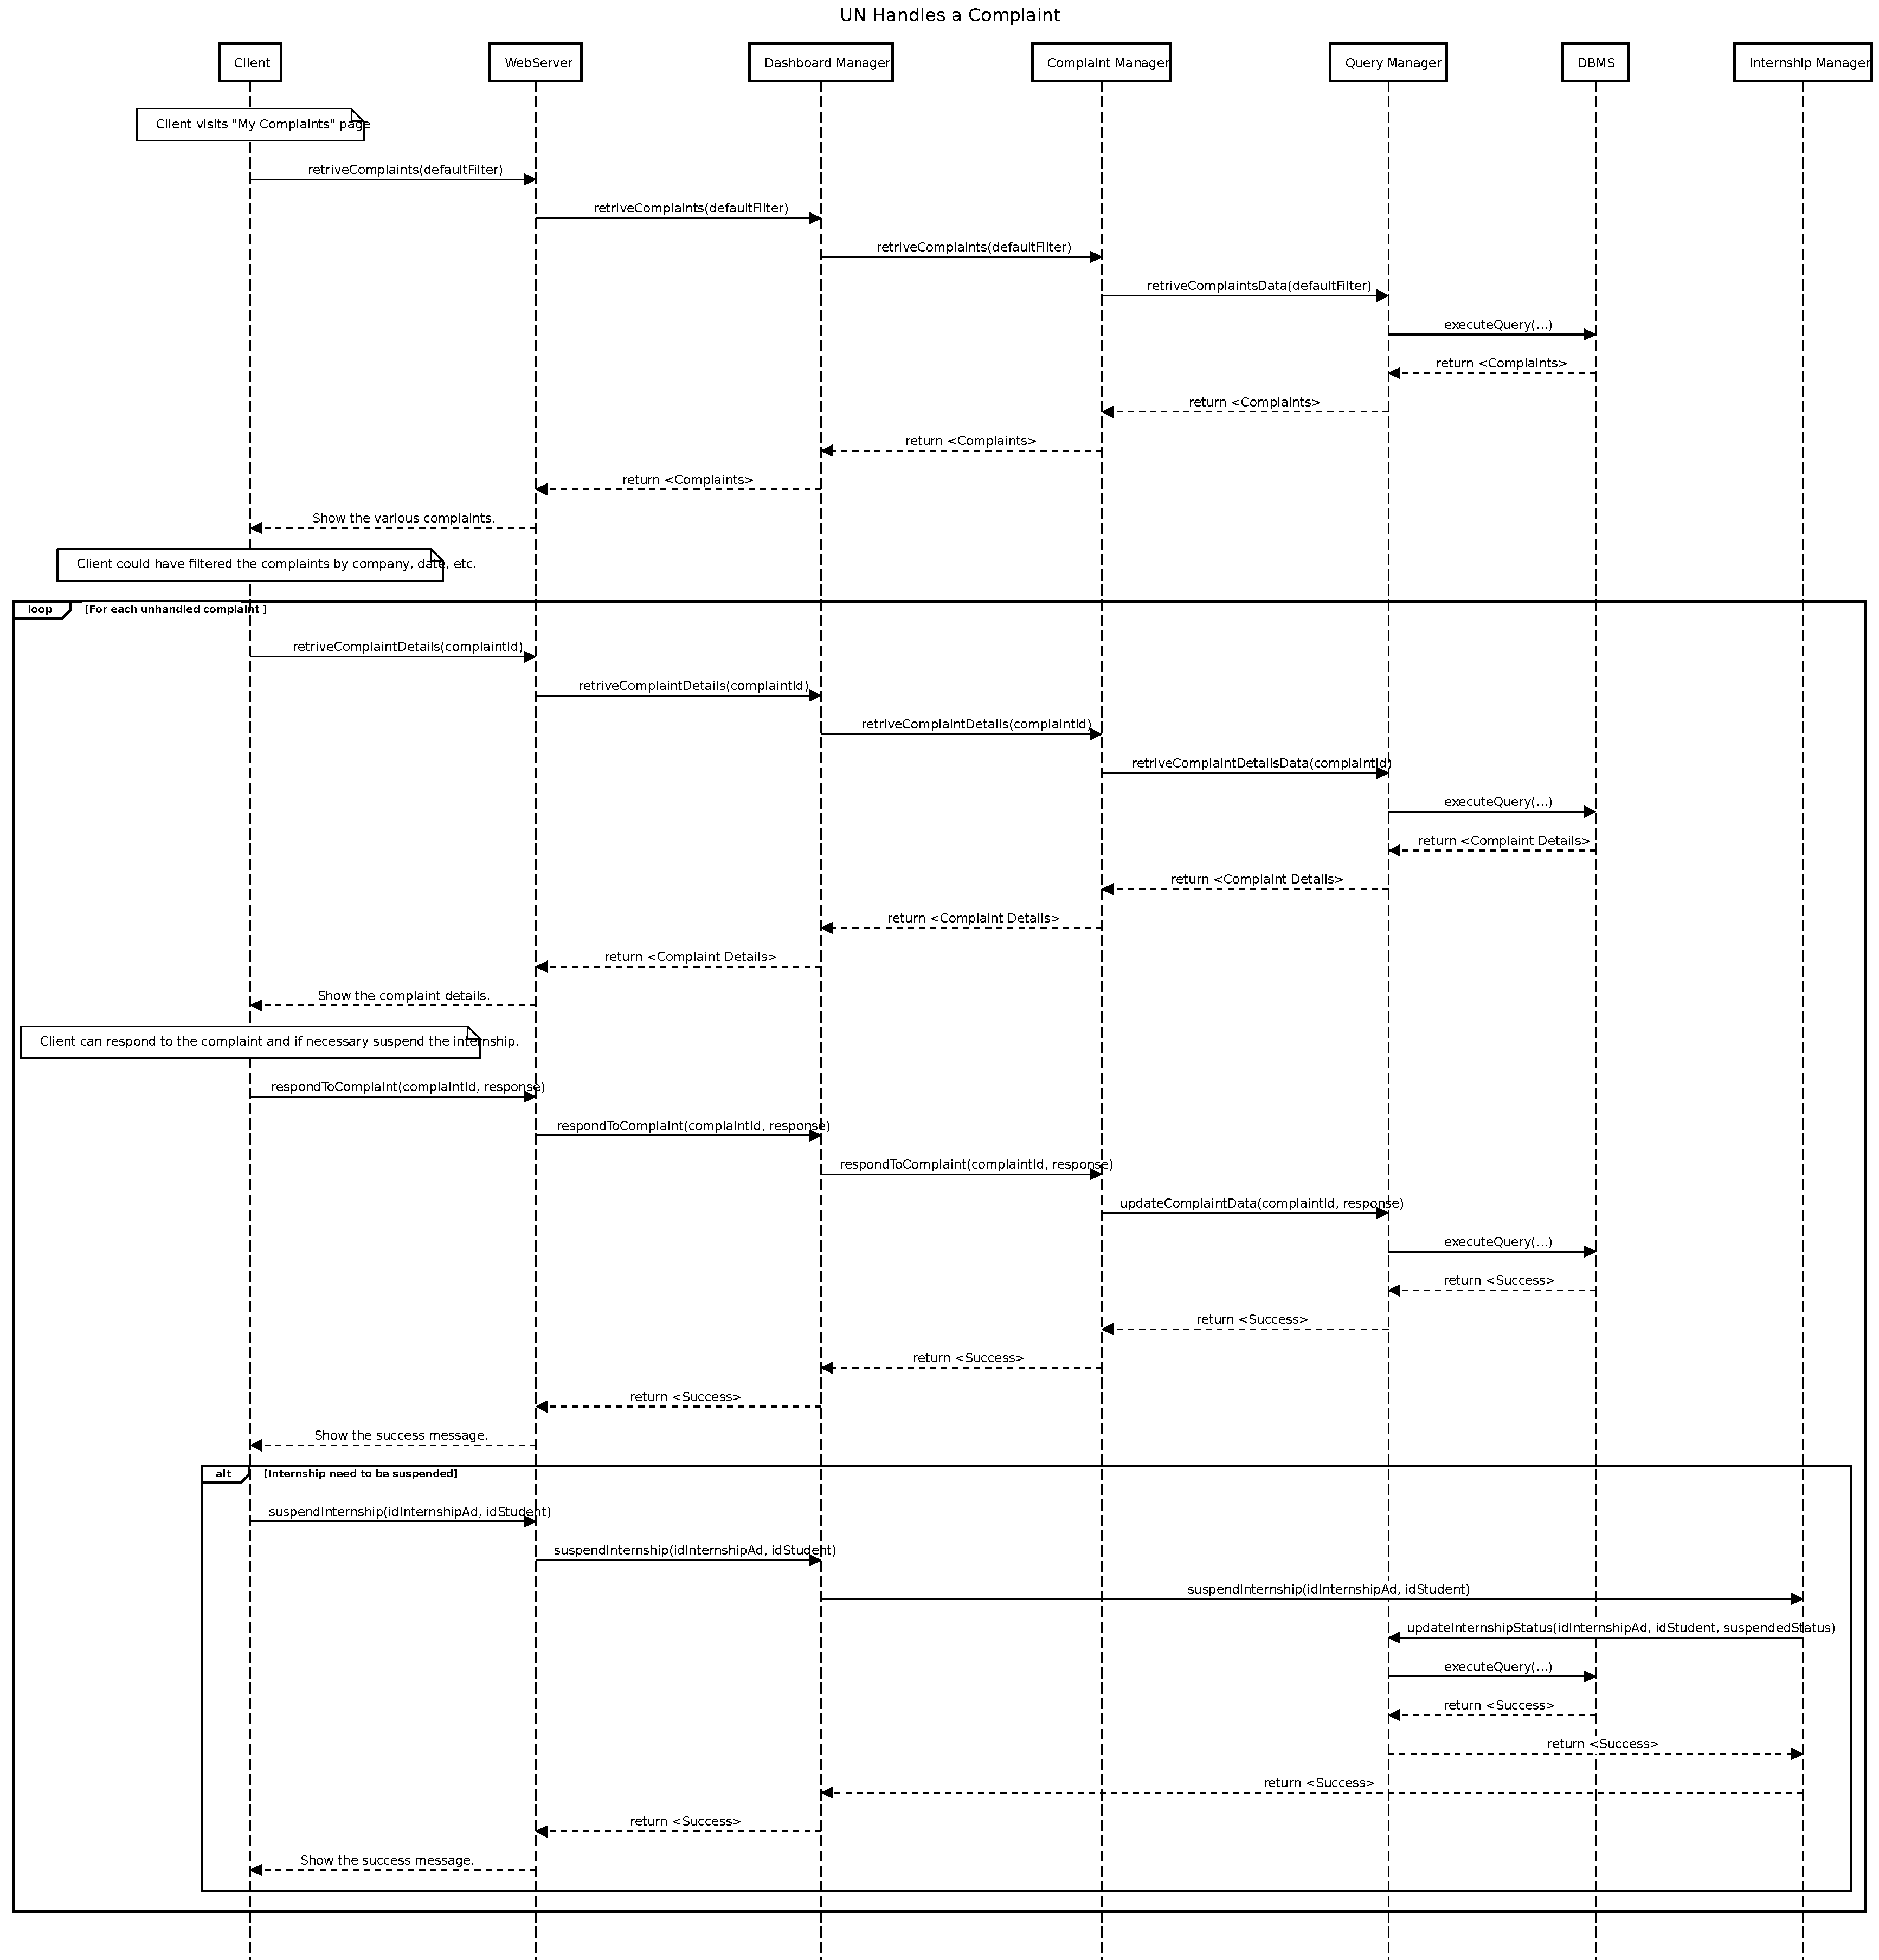
\includegraphics[width=1.0\textwidth]{Images/RV_13.pdf}
      \caption{Runtime View - University handles a complaint}
      \label{fig:rv-un-handles-complaint}
\end{figure}

\par This sequence diagram illustrates how a UN can handle a complaint. The client is on the "My Complaints" page. The
S\&C server retrieves the list of "active" complaints that the UN is involved in and sends it to the client. The UN can
then see the status of each complaint and - if needed - can filter the list by company, or other criteria.

\par The UN can then click on a complaint to see the details. The S\&C server retrieves the complaint details and sends
it back to the client. The UN can then see the complaint and the related internship. UN can respond to the complaint
and also suspend the internship if necessary. The S\&C server saves the changes made and sends a confirmation message
to the UN after each action.

% RV 14
\subsection{University blocks a malicious company}
\label{sub:university-blocks-a-malicious-company}%

\begin{figure}[H]
      \centering
      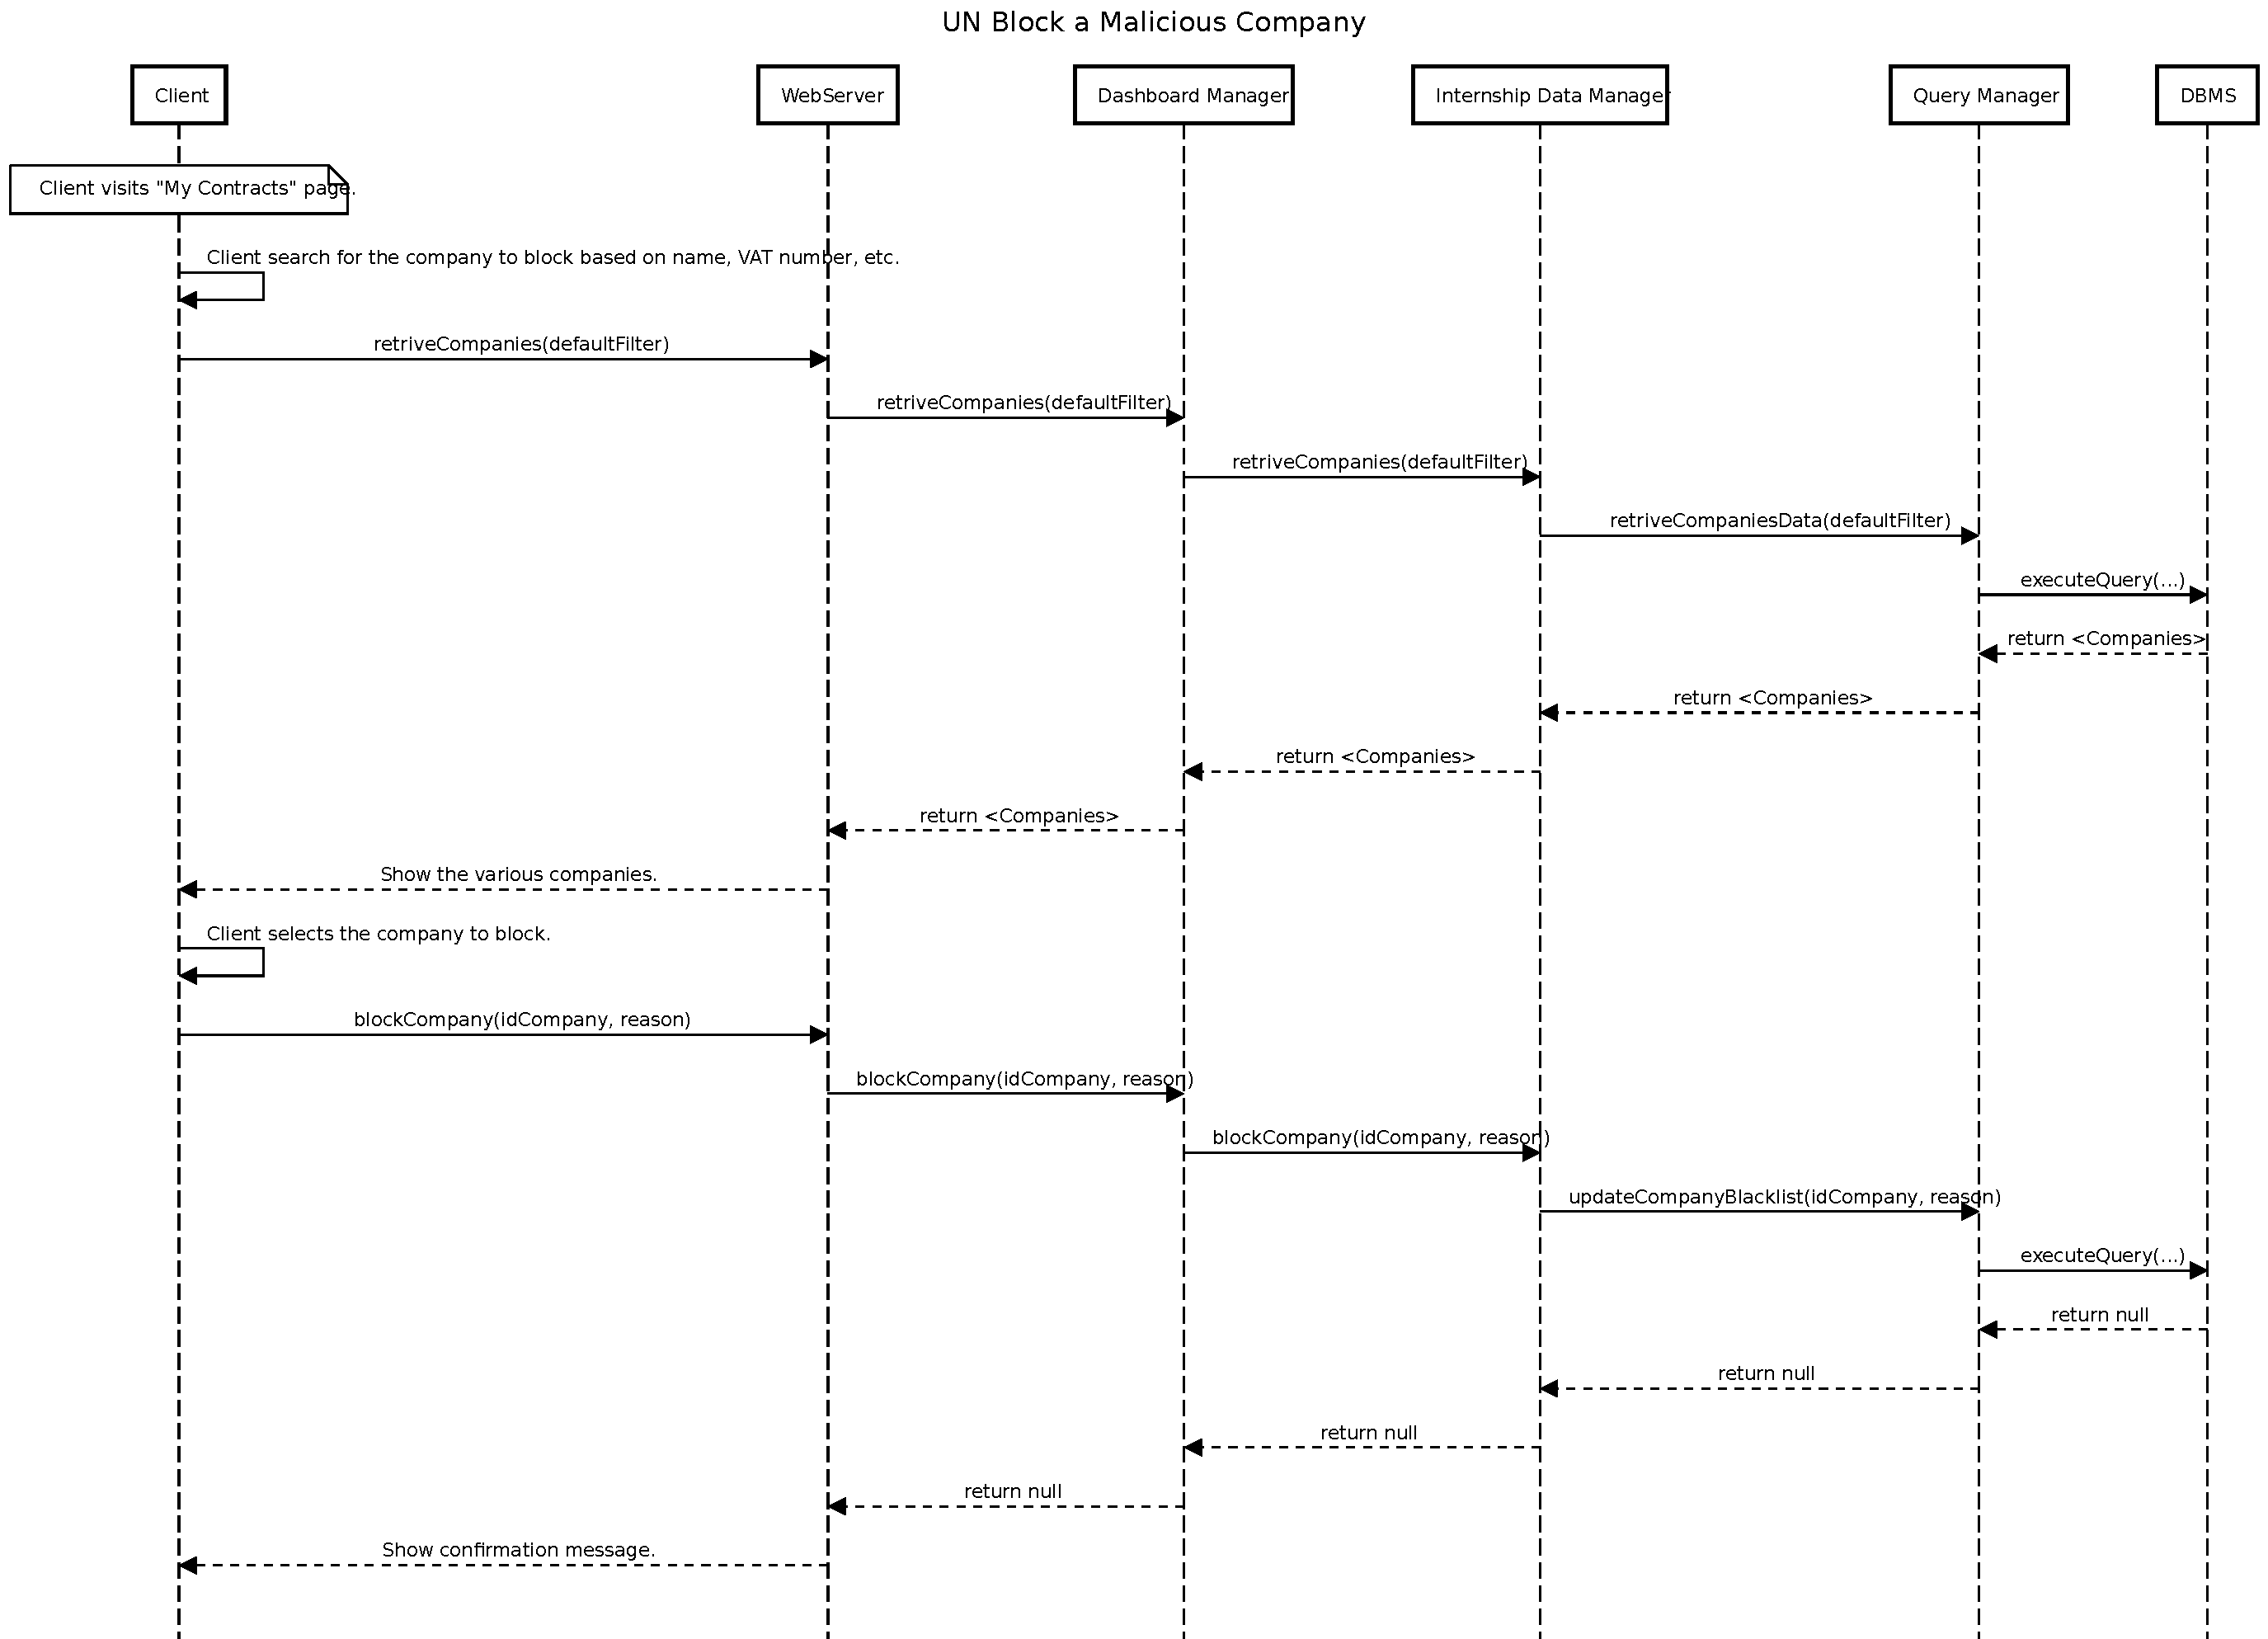
\includegraphics[width=1.0\textwidth]{Images/RV_14.pdf}
      \caption{Runtime View - University blocks a malicious company}
      \label{fig:rv-un-blocks-company}
\end{figure}

\par This sequence diagram illustrates how a UN can block a malicious company. The client is on the "My Contracts" page
and clicks on the "Block Company" button. The client shows a search bar where the UN can search for the company to
block using the company's name, VAT number, or other criteria. The S\&C server retrieves the list of companies that
match the search criteria and sends it to the client. The UN can then select the company to block and clicks on the
"Block" button. The S\&C server adds the company to the blacklist and sends a confirmation message to the UN.

\section{Component Interfaces}
\label{sec:component-interfaces}%

\begin{itemize}
      \item \textbf{Login Manager}:
          \begin{itemize}
              \item LoginAtUniversity(String unId)
              \item sendInfo(STInfo stInfo)
              \item validateCredential(String username, String password)
          \end{itemize}
  
      \item \textbf{Internship Manager}
          \begin{itemize}
              \item requestSnipped(List<String> internIds)
              \item internshipSearch(SearchParameters searchParams)
              \item retrieveSTInternship(String stId)
              \item storeInternshipAd(InternshipAd internshipAd)
          \end{itemize}
  
      \item \textbf{Profile Manager}
          \begin{itemize}
              \item archiveCV(File CV)
          \end{itemize}
      
      \item \textbf{Questionnaire Manager}
          \begin{itemize}
              \item compileQuestionnaire(String idInternshipAd)
              \item answerCOQuestionnaire(Answer answer)
              \item compileFeedbackQuestionnaire(String idInternshipAd)
              \item answerFeedbackQuestionnaire(Answer answer)
          \end{itemize}
  
      \item \textbf{Complaint Manager}
          \begin{itemize}
              \item createAndNotifyComplaint(String stId, String universityId, Complaint complaint)
          \end{itemize}
  
      \item \textbf{Notification Manager}
          \begin{itemize}
              \item newComplaintAdded(String universityId, String companyId)
          \end{itemize}
  
      \item \textbf{Recommendation Manager}
          \begin{itemize}
              \item retrieveRecommendation(String stId, SearchParameters searchParams)
          \end{itemize}
  
      \item \textbf{Suggestion Manager}
          \begin{itemize}
              \item feedCVToEngine(File CV)
              \item feedInternAdToEngine(InternshipAd internshipAd)
          \end{itemize}
  
      \item \textbf{Query Manager}
          \begin{itemize}
              \item retrieveInfo(String userId)
              \item linkInfoToId(String userId, STInfo stInfo)
              \item credentialStored(String username)
              \item archiveCV(File CV)
              \item requestSnipped(List<String> internIds)
              \item internshipSearch(SearchParameters searchParams)
              \item retrieveQuestionnaireData(String idInternshipAd)
              \item saveSTAnswer(Answer answer)
              \item retrieveSTInternship(String stId)
              \item storeInternshipAd(InternshipAd internshipAd)
          \end{itemize}
  
      \item \textbf{Dashboard Manager}
          \begin{itemize}
              \item LoginAtUniversity(String unId)
              \item sendInfo(STInfo stInfo)
              \item sendCredential(String username, String password)
              \item initiateSearch(SearchParameters searchParams)
              \item compileQuestionnaire(String idInternshipAd)
              \item answerCOQuestionnaire(Answer answer)
              \item compileFeedbackQuestionnaire(String idInternshipAd)
              \item answerFeedbackQuestionnaire(Answer answer)
              \item retrieveSTInternship(String stId)
              \item createComplaint(String stId, String universityId, Complaint complaint)
              \item addComplaint(String stId, Complaint complaint)
              \item createInternshipAd(InternshipAd internshipAd)
          \end{itemize}
  
  \end{itemize}

\section{Selected Architectural Styles and Patterns}
\label{sec:selected-architectural-styles-patterns}%

\par{\textbf{Architectural Design:}} The architectural design of S\&C is based on the industry-standard 3-Tier-Architecture pattern:

\begin{enumerate}
      \item \textbf{Presentation Tier:} This is the upper layer that directly interacts with users. The presentation tier
            focuses on displaying information to the user and capturing user inputs. It's designed to handle all client-side
            interactions and renders the application's visual components.
      \item \textbf{Application Tier:} This layer contains the core business logic and processing rules of the
            application. It receives requests from the presentation tier, applies business rules, validates data, and
            coordinates the flow of information. This tier acts as an intermediary, ensuring that data is processed
            according to the application's specific requirements before being passed to or retrieved from the data tier.
      \item \textbf{Data Tier:} The bottom layer of the architecture, responsible for storing, retrieving, and managing
            data. The data tier ensures data integrity, provides database connection management, and implements data
            access methods that the application tier can use to interact with the stored information.
\end{enumerate}

The division of the system into these three layers allows a reduction in complexity, improves maintainability, and
facilitates scalability: each layer can be developed, tested, deployed and maintained independently, enabling a more
modular and flexible system architecture while also paralleling development efforts.

The choice of a 3-Tier-Architecture is also motivated by the fact that it can be easily mapped to the MVC
(Model-View-Controller) pattern - a widely-used design pattern that separates the application into three interconnected
components: the Model (data), the View (interface), and the Controller (business logic). This pattern is particularly
useful since it allows for a clear separation of concerns and a more modular and maintainable codebase.

With this knowledge in mind, the services division shown in the Deployment Diagram (\ref{fig:deployment-diagram}) can
be easily understood: the Web Server is the presentation tier, the S\&C Server is the application tier, and the DBMS
Server is the data tier. The other services are additional components that provide extra functionalities to the system.

\par{\textbf{Client-Server Communication:}} S\&C - like almost all modern web applications - is based on a
Client-Server architecture. The client (the user's browser) sends requests to the server, which processes them and
returns the appropriate responses. All the static content (HTML, CSS, JavaScript) is served directly using HTTPS, while
the dynamic content is generated by the server and sent back to the client as JSON data (REST over HTTPS) to be
rendered by the client-side JavaScript code.

\par{\textbf{Server-Server Communication:}} The communication between the presentation tier and the application tier
will be based on REST API. The communication between the application tier and the data tier will be based on SQL
Queries over TCP/IP (as implemented by the database driver).

\section{Other Design Decisions}
\label{sec:other-design-decisions}%

\par{\textbf{Auxiliary Components:}} In \ref{sec:selected-architectural-styles-patterns} we said that the application
tier of S\&C is composed of the S\&C Server but, in reality, the core application depends on other auxiliary services
that provide additional functionalities. These services are:

\begin{itemize}
      \item \textbf{Email Service:} Communicates with the core using SMTP over TCP/IP. Core prepares the email and
            "tasks" the service to deliver it to the recipient.
      \item \textbf{Recommendation Engine:} A service that provides internships recommendations to STs and anonymized
            CVs to COs. Communicates with the core using REST API. Core asks the Recommendation Engine for
            recommendations and service provides them.
      \item \textbf{Suggestion Engine:} A service that provides suggestions to improve CVs and Internship
            Advertisements. Communicates with the core using REST API. Core asks the Suggestion Engine for suggestions
            and service provides them.
\end{itemize}

It must also be noted that the core application communicates with the various UNs' SSOs using REST API. These portals
are not under S\&C control and are considered external services.

The choice of not having a fully-integrated monolithic application is motivated by these reasons:

\begin{itemize}
      \item \textbf{Scalability:} The Suggestion and Recommendation Engines can be scaled independently from the core
            application. This is useful since the load on these services is expected to be higher than on the core
            application due to the complexity of the algorithms they run.
      \item \textbf{Make-vs-Buy:} The Email Service is a commodity service and open source solutions are available.
            It's more cost-effective to use an existing solution than to develop a custom one.
\end{itemize}

\par{\textbf{Orchestration:}} The various services will be orchestrated using Kubernetes. This choice is motivated by
the fact that Kubernetes is the industry standard for container orchestration and provides a robust and scalable
solution for managing containerized applications.

The presence of orchestrators node is implicit and as such is not shown in the Deployment Diagram
(\ref{fig:deployment-diagram}). An orchestrator can also be bought as a service from cloud providers thus making it
outside the scope of the S\&C system.  Also, an orchestrator can be superfluous in a small-scale deployment
such as the one used in the testing environment.

\par{\textbf{Networking:}} In the Deployment Diagram (\ref{fig:deployment-diagram}) the cluster LAN is separated from
the outside world by a firewall acting as a gateway. This is a common practice to protect the internal network from
malicious attacks by filtering incoming traffic. The firewall can be a physical device or a virtual one, depending on
the deployment environment. In a cloud environment, the firewall can be a virtualized service provided by the cloud
provider.

In case of a multi-tenant deployment, the firewall should be replicated and will act as a router between the various
clusters connected to each other in a fully-meshed topology using L3VPN and dynamic routing protocols. However, this
is outside the scope of the S\&C system.
